\documentclass[11pt]{book} % 11pt font
\usepackage{amsmath}
\usepackage{amsfonts}
\usepackage{bm}
\usepackage{graphicx}
\usepackage{mathtools}
\usepackage{physics}
\usepackage{pgfplots}
\usepackage{accents}
\usepackage{geometry}
\usepackage{caption}

% my custom commands
% ------------------
% note command
\newcommand{\note}[1]{\textsf{\textcolor{red}{#1}}}
% multi-line comment command
\newcommand{\comment}[1]{}
\newcommand{\del}{\bm{\nabla}}
\newcommand{\partder}[2]{\frac{\partial #1}{\partial #2}}
\newcommand{\compcon}{\text{c.c}}
\newcommand{\hercon}{\text{h.c.}}
\newcommand{\vac}{\ket{\text{vac}}}
\newcommand{\vacb}{\bra{\text{vac}}}
\DeclareMathOperator{\sinc}{sinc}
\graphicspath{{./images}}


% -------------------------
% BEGINNING OF THE DOCUMENT
% -------------------------
\begin{document}

\chapter{Fall Term, Hailin Wang}
\section{Overview}
The start of the course will mainly focus on two level states (5-6 weeks) and then we move on to 3 level states and the mechanical effects of light. \\
This course will focus on how does light interact with matter.\\
This interaction can be done in terms of semi-classical physics, where we have classical light and quantum mechanical matter, or a pure quantum approach which treats both light and matter quantum mechanically.\\

\section{Two-Level quantum systems (aka the Rabi problem)}
In a simple system we have discrete atomic energy levels and a single opticla mode of light:
\begin{align*}
	\frac{1}{2} E_0 e^{-i\omega t} + \text{c.c.}
\end{align*}
But this discrete set of atomic energy levels is still too complicated since there are an infinite number of states for the atom. In order to further simplify things we limit ourselves to two-level systems where our atom can be in state $\ket{1}$ or $\ket{2}$.\\
If we have transition energy between the two states that has a corresponding energy $\omega_0$ and an optical field at $\omega$, we then have a detuning $\delta = \omega_0-\omega$, resonance when $\omega=\omega_0$, and near resonance when $\omega\approx\omega_0$.\\
When we are near resonance we ignore all off-resonant interactions.\\
We now come up with our Hamiltonian (after which we will try to solve the Schroedinger equation).
\begin{align*}
	H &= H_0 + V \\
	H_0 &= \begin{pmatrix} E_1 & 0 \\ 0 & E_2\end{pmatrix} \\
	H_0 &= \hbar\begin{pmatrix} \omega_1 & 0 \\ 0 & \omega_2\end{pmatrix}
\end{align*}
We now use the fact that $\omega_1 - \omega_2 = \omega_0$, so we rewrite this as:
\begin{align*}
	H_0 &= \frac{\hbar}{2}\begin{pmatrix} -\omega_0 & 0 \\ 0 & \omega_0\end{pmatrix} \\
	H_0 &= -\frac{\hbar\omega_0}{2}\begin{pmatrix} 1 & 0 \\ 0 & -1\end{pmatrix}
\end{align*}
Since atoms are neutral, if our wavelength is much larger than the bohr radius we can model this with a dipole interaction.\\
Our dipole potential is:
\begin{align*}
	V &= -\bm{\mu}\cdot\bm{E} \\
	\bm{\mu} &= -e\bm{r} \\
	\bm{E} &= |E_0| \cos(\omega t-\phi)\hat{\epsilon}
\end{align*}
We could in principle add a quadrapole, magnetic dipole interaction, etc.\\
If we have our field point allong the z axis we can write:
\begin{align*}
	V_{12} &= \bra{1} V\ket{2} \\
	V_{12} &= e Z_{12} |E_0| \cos(\omega t -\phi) \\
	V_{11} &= \bra{1} V\ket{1} \\
	V_{11} &= e Z_{11} |E_0| \cos(\omega t -\phi) \\
	V_{22} &= \bra{2} V\ket{2} \\
	V_{22} &= e Z_{22} |E_0| \cos(\omega t -\phi)
\end{align*}
But we know $Z_{11} = Z_{22} = 0$ by symettry (though this may not hold inside some crystals). \\
Therefore we can then write:
\begin{align*}
	V &= \begin{pmatrix} V_{12} & 0 \\ 0 & V_{21} \end{pmatrix}
\end{align*}
We define $\Omega_0$ (the Rabi frequency).
\begin{align*}
	\Omega_0 &= -\frac{\mu_{12} E_0}{\hbar}
\end{align*}
By convention we choose the phase of $\mu_{12} = -e Z_{12}$ to make it real. Therefore we have:
\begin{align*}
	V_{12} &= \hbar |\Omega_0| \cos (\omega t -\phi) \\
	V &= \hbar |\Omega_0| \cos (\omega t - \phi)\begin{pmatrix}
		0 & 1 \\
		1 & 0
      \end{pmatrix}
\end{align*}
In terms o the Pauli matricies we then have:
\begin{align*}
	H_0 &= -\frac{\hbar\omega_0}{2} \sigma_z \\
	V &= \hbar |\Omega_0|\cos(\omega t - \phi) \sigma_x \\
	H &= -\frac{\hbar\omega_0}{2} \sigma_z + \hbar |\Omega_0|\cos(\omega t - \phi) \sigma_x
\end{align*}
The key parameters in question for this hamiltonian are the detuning, $\delta=\omega_0-\omega$ and the Rabi frequency $\Omega_0$. \\
\subsection{Interaction representation and rotating wave approximation}
In the Schroedinger representation:
\begin{align*}
	\ket{\psi(t)} &= \sum_n c_n(t) \ket{n} \\
	i\hbar \partial_t \ket{\psi(t)} &= H\ket{\phi(t)}
\end{align*}
If we assume that we have a phase of zero, so $\Omega_0$ is real:
\begin{align*}
	i\hbar \partial_t \begin{pmatrix}c_1 \\ c_2\end{pmatrix} &= H \begin{pmatrix}c_1 \\ c_2\end{pmatrix} \\
	i\hbar \partial_t \begin{pmatrix}c_1 \\ c_2\end{pmatrix} &= \hbar \begin{pmatrix} -\frac{\omega_0}{2} & \Omega_0 \cos\omega t \\ \Omega_0\cos\omega t & \frac{\omega_0}{2}\end{pmatrix} \begin{pmatrix}c_1 \\ c_2\end{pmatrix} \\
	\dot{c_1} &= i \frac{\omega_0}{2} c_1 - i\Omega_0\cos\omega t c_2 \\
	\dot{c_2} &= i \frac{\omega_0}{2} c_2 - i\Omega_0\cos\omega t c_1
\end{align*}
If $\Omega_0 = 0$ we just get free evolution, so we only have phase evolution for both terms. \\
In the interaction representation we put the evolution from $H_0$ into the states, so:
\begin{align*}
	\ket{\psi(t)} &= \sum_n \bar{c_n}(t) e^{-i \omega_n t} \ket{n}
\end{align*}
So our equation of motion becomes:
\begin{align*}
	i \hbar \partial_t \begin{pmatrix}\bar{c_1} \\ \bar{c_2} \end{pmatrix} &= V_I \begin{pmatrix}\bar{c_1} \\ \bar{c_2}\end{pmatrix}
\end{align*}
We know from our definitions for the interaction picture:
\begin{align*}
	\bar{c_n} &= c_n e^{i\omega_n t} \\
	\dot{\bar{c_n}} &= \dot{c_n} e^{i\omega_n t} + i\omega_n c_n e^{i\omega_n t} \\
	\dot{\bar{c_1}} &= \left(i \frac{\omega_0}{2} c_1 - i\Omega_0\cos\omega t c_2 \right) e^{-i\frac{\omega_0}{2} t} -\frac{i\omega_0}{2}c_1 e^{-i\frac{\omega_0}{2} t} \\
	\dot{\bar{c_1}} &= - i\Omega_0\cos\omega t c_2  e^{-i\frac{\omega_0}{2} t} \\
	\dot{\bar{c_1}} &= -i\Omega_0\cos\omega t \bar{c_2}e^{-i\omega_0 t} \\
	\dot{\bar{c_2}} &= -i\Omega_0\cos\omega t \bar{c_1} e^{i\omega_0 t}
\end{align*}
Therefore:
\begin{align*}
	V_I &= \hbar \Omega_0 \cos\omega t \begin{pmatrix}
		0 & e^{-i\omega_0 t} \\
		e^{i\omega_0 t} & 0
		\end{pmatrix}
\end{align*}
So working in the interaction picture here has simply removed the diagonal part of the Hamiltonian. \\
We now seek to solve our equations for our amplitudes here, we start be rewriting cosine in terms of complex exponentials:
\begin{align*}
	\dot{\bar{c_1}} &= -i\frac{\Omega_0}{2}\left(e^{i\omega t} + e^{-i\omega t}\right)e^{-i\omega_0 t}\bar{c_2} \\
	\dot{\bar{c_1}} &= -i\frac{\Omega_0}{2}\left(e^{i(\omega-\omega_0) t} + e^{-i(\omega+\omega_0) t}\right)\bar{c_2} \\
	\dot{\bar{c_2}} &= -i\frac{\Omega_0}{2}\left(e^{i\omega t} + e^{-i\omega t}\right)e^{i\omega_0 t}\bar{c_1} \\
	\dot{\bar{c_2}} &= -i\frac{\Omega_0}{2}\left(e^{i(\omega_0-\omega) t} + e^{i(\omega + \omega_0)t}\right)\bar{c_1}
\end{align*}
We now break this into a perurbation series:
\begin{align*}
	\bar{c_n} &= \bar{c}_n^{(0)} + \bar{c}_n^{(1)} +\bar{c}_n^{(2)} + \ldots \\
	\bar{c}_n^{(m)} &\propto E_0^m 
\end{align*}
If we start in state 1:
\begin{align*}
	\dot{\bar{c}_1^{(1)}} &\propto \bar{c}_2^{(0)} = 0 \\
	\dot{\bar{c}_2^{(1)}} &=-i\frac{\Omega_0}{2}\left(e^{i(\omega_0 - \omega) t} + e^{i(\omega_0 + \omega)t}\right)
\end{align*}
So we have after integration:
\begin{align*}
	\bar{c}_2^{(1)}(t) &= -i\frac{\Omega_0}{2} \left[ \frac{e^{i\omega_0-\omega)t} -1 }{i(\omega_0-\omega} + \frac{e^{i(\omega_0 + \omega) t} - 1}{i(\omega_0 + \omega)}\right]
\end{align*}
If we are near resonance the second term is much smaller, and $\Omega_0 << \omega_0$ we use the rotating wave approximation:
\begin{align*}
	\bar{c}_2^{(1)}(t) &= -i\frac{\Omega_0}{2}\frac{e^{i\omega_0-\omega)t} -1 }{i(\omega_0-\omega} 
\end{align*}
Which equivalently in the hamiltonian has:
\begin{align*}
	V_I &= \hbar \frac{\Omega_0}{2} \begin{pmatrix}
		0 & e^{-i\delta t} \\
		e^{i\delta t} & 0
		\end{pmatrix}
\end{align*}
If we generalize we have (with some phase on $\Omega_0$):
\begin{align*}
	V_I &= \frac{\hbar }{2} \begin{pmatrix}
		0 & \Omega_0^*e^{-i\delta t} \\
		\Omega_0e^{i\delta t} & 0
		\end{pmatrix}
\end{align*}
\subsection{The exact solution of the Rabi problem (with rotating wave approximation)}
Next class we will solve this, we will get $\pi$ pulses, Rabi oscilations, etc.

\subsection{Review of last class}
In the interaction between a 2 level system and an optical field, we have an interaction potential $V= -\bm{\mu}\cdot\bm{E}$. We worked in the interaction picture, which removed the free interaction dependance from our states (at the cost of making our interaction potential slightly more complicated). We then made the rotating wave approximation, where we drop all counter rotating terms from the interaction potantial.
\subsection{Rabi Problem and the exact solution}
We define the spin-flip opertors:
\begin{align*}
	\sigma_+ &= \begin{pmatrix}
		0 & 0 \\
		1 & 0
	     \end{pmatrix} \\
	\sigma_- &= \begin{pmatrix}
		0 & 1 \\
		0 & 0
	     \end{pmatrix}
\end{align*}
So we can then write our interaction potential as:
\begin{align*}
	V_I &= \frac{\hbar}{2} \Omega_0 e^{i\delta t} \sigma_+ + \text{h.c.}
\end{align*}
And we know:
\begin{align*}
	\sigma_+ \ket{1} &= \ket{2} \\
	\sigma_+ \ket{2} &= 0 \\
	\sigma_- \ket{2} &= \ket{1} \\
	\sigma_- \ket{1} &= 0
\end{align*}
We now try to solve our equation for some special cases. If we pick exact resonance, so our detuning is zero, and a constant $\Omega_0$ we have:
\begin{align*}
	\dot{\bar{c}}_1 &= -\frac{i\Omega_0}{2} \bar{c}_2 \\
	\ddot{\bar{c}}_1 &= -\frac{\Omega_0^2}{4} \bar{c}_1 \\
	\dot{\bar{c}}_2 &= -\frac{i\Omega_0}{2} \bar{c}_1 \\
	\ddot{\bar{c}}_2 &= -\frac{\Omega_0^2}{4} \bar{c}_2
\end{align*}
This emits solutions in the form of sines and cosines. If we assume the population starts in state $\ket{1}$ we have:
\begin{align*}
	\bar{c}_1 &= \cos\left(\frac{\Omega_0}{2} t\right) \\
	\bar{c}_2 &= -i\sin\left(\frac{\Omega_0}{2} t\right)
\end{align*}
Since the probability is the square of the amplitude we have oscilations between the states with frequency $\Omega_0$.

If instead we have a variable $\Omega_0$ but exact resonance we have a more difficult problem to solve. In order to solve this we define:
\begin{align*}
	\bar{c}_\pm &= \bar{c}_1 \pm \bar{c}_2 \\
	\dot{\bar{c}}_+ &= -i\frac{\Omega_0}{2} \bar{c}_+ \\
	\dot{\bar{c}}_- &= i\frac{\Omega_0}{2} \bar{c}_-
\end{align*}
So our solutions are:
\begin{align*}
	\bar{c}_+(t) &= \bar{c}_+(0) e^{-i\int_0^t dt' \frac{\Omega_0}{2}} \\
	\bar{c}_-(t) &= \bar{c}_-(0) e^{i\int_0^t dt' \frac{\Omega_0}{2}}
\end{align*}
We now define the pulse area:
\begin{align*}
	A(t) &= \int_0^t dt' \Omega_0(t)
\end{align*}
So:
\begin{align*}
	\bar{c}_+(t) &= \bar{c}_+(0) e^{-\frac{i}{2}A(t)} \\
	\bar{c}_-(t) &= \bar{c}_-(0) e^{\frac{i}{2}A(t)}
\end{align*}
So then:
\begin{align*}
	\begin{pmatrix}
		\bar{c}_1(t) \\
		\bar{c}_2(t)
	\end{pmatrix} &= \begin{pmatrix}
	\cos\frac{A}{2} & -i\sin\frac{A}{2} \\
	-i\sin\frac{A}{2} & \cos\frac{A}{2}
		  \end{pmatrix}
		  \begin{pmatrix}
			  \bar{c}_1(0) \\
			  \bar{c}_2(0)
    \end{pmatrix}
\end{align*}
Which corresponds to oscilatory behavior, but with respect to the pulse area rather than time.\\
We can therefore talk about a $\pi$ pulse, which has a total pulse area of $\pi$, aka $\lim_{t\to\infty} A(t) = \pi$. This will cause the population to swap and gain a phase of $-i$.\\
Similarly a $2\pi$ pulse will only add an overall $-1$ phase to both $\bar{c}_1$. This is a Berry phase. \\
We finally consider a non-zero detuning with a constant Rabi frequency:
\begin{align*}
	\ddot{\bar{c}}_1 &= -i\delta\dot{\bar{c}}_1  - \frac{\Omega_0^2}{4} \bar{c}_1 \\
\ddot{\bar{c}}_2 &= i\delta\dot{\bar{c}}_2  - \frac{\Omega_0^2}{4} \bar{c}_2
\end{align*}
These emit complex exponential solutions, our solution is therefore:
\begin{align*}
	\Omega &= \sqrt{\Omega_0^2 + \delta^2} \\
	\gamma &= -\frac{i\delta}{2} \pm i\frac{\Omega}{2}
	\bar{c}_1 &= \bar{c}_1(0) e^{\gamma t}
\end{align*}
$\Omega$ is the generalize Rabi frequency. Our solution is therefore:
\begin{align*}
	\bar{c}_1 &= e^{i\frac{\delta}{2} t} \left[ B_1 \cos \frac{\Omega t}{2} + B_2 \sin \frac{\Omega t}{2}\right] \\
	\bar{c}_2 &= \frac{\dot{\bar{c}}_1}{-i\frac{\Omega_0}{2} e^{-i\frac{\delta}{2} t}} \\
	\bar{c}_2 &= e^{i\frac{\delta}{2} t} \left[ B_1 \sin \frac{\Omega t}{2} + B_2 \cos \frac{\Omega t}{2}\right]
\end{align*}
If we start with our population in state 1, then:
\begin{align*}
	|\bar{c}_2(t)|^2 &= \left(\frac{\Omega_0}{\Omega}\right)^2 \sin \frac{\Omega t}{2} \\
\end{align*}
If we return to the Schroedinger represntation, we see that the energy levels appear to be shifting due to this applied optical field. This is known as the optical Stark shift.\\
So far we have assumed this is a perfect system, if we assume that we can actually decay out of the system, we have:
\begin{align*}
	\partial_t |\bar{c}_1|^2 &= -\gamma_2|\bar{c}_1|^2 \\
	\partial_t |\bar{c}_2|^2 &= -\gamma_2|\bar{c}_2|^2
\end{align*}
This corresponds to a decay term that is half the given rate in the amplitude. We can seey this bay taking the onsatz that it is half and quckly see this is true:
\begin{align*}
	\partial_t \bar{c}_1 &= -\frac{\gamma_1}{2} \bar{c}_1 \\
	\partial_t |\bar{c}_1|^2 &= \dot{\bar{c}}_1\bar{c}_1^* + \bar{c}_1 \dot{\bar{c}}_1^* \\
	\partial_t |\bar{c}_1|^2 &= \frac{\gamma}{2}\bar{c}_1\bar{c}_1^* + \frac{\gamma}{2}\bar{c}_1 \bar{c}_1^* \\
	\partial_t |\bar{c}_1|^2 &= \gamma |\bar{c}_1|^2
\end{align*}
\subsection{Field interaction representation/ rotating frame}
In the Schroedinger represntation:
\begin{align*}
	\ket{\psi} &= \sum_n c_n \ket{n} \\
	H\ket{n} &= \hbar\omega_n\ket{n}
\end{align*}
In the interaction represntation
\begin{align*}
	\ket{\psi} &= \sum_n \bar{c}_n e^{-i\omega_n t}\ket{n} \\
\end{align*}
In a two level system:
\begin{align*}
	i\hbar\partial_t \begin{pmatrix}
		\bar{c}_1 \\
		\bar{c}_2 
	\end{pmatrix} &= V_I \begin{pmatrix}
	\bar{c}_1 \\
	\bar{c}_2
		      \end{pmatrix}
	V_I &= \frac{\hbar}{2} \begin{pmatrix}
		0 & \Omega_0^* e^{-i\delta t} \\
		\Omega_0 e^{i\delta t} & 0
			\end{pmatrix}
\end{align*}
In order to work with a time-independant H, we pick a new set of coefficients:
\begin{align*}
	\ket{\psi} \tilde{c}_1 e^{i\frac{\omega}{2} t} \ket{1} + \tilde{c}_2 e^{i\frac{\omega}{2} t}\ket{2}
\end{align*}
So:
\begin{align*}
	\tilde{c}_1 &= \bar{c}_1 e^{i\frac{\delta}{2} t} \\
	\tilde{c}_2 &= \bar{c}_2 e^{-i\frac{\delta}{2} t} \\
	\dot{\tilde{c}}_1 &= i\frac{\delta}{2} \tilde{c}_1 -\frac{i\Omega_0^*}{2} \tilde{c}_2 \\
	\dot{\tilde{c}}_2 &= -i\frac{\delta}{2} \tilde{c}_2 -\frac{i\Omega_0}{2} \tilde{c}_1
\end{align*}
So our Hamiltonian becomes:
\begin{align*}
	i\hbar \partial_t \begin{pmatrix}
		\tilde{c}_1 \\
		\tilde{c}_2 
	\end{pmatrix} &= \tilde{H} \begin{pmatrix}
\tilde{c}_1 \\
\tilde{c}_2
			    \end{pmatrix} \\
	\tilde{H} &= -\frac{\hbar\delta}{2} \begin{pmatrix}
		1 & 0 \\
		0 & -1
	\end{pmatrix} + \frac{\hbar}{2} \begin{pmatrix}
		0 & \Omega_0^* \\
		\Omega_0 & 0
				 \end{pmatrix}
\end{align*}
This looks like a frequency difference between the two states, but with a D.C. coupling between the states. This is different from the interaction picture where we remove the frequency difference but keep an ac transition, or the Schroedinger picture where we have a frequncy difference and AC coupling.
\subsection{Next week}
Unitary transformations, solving $\tilde{H}$ to find it's eigenstates (in the field interaction representation). These states are the semi-classical dressed states. This also relates to optical stark effects and optical stark splitting.

\subsection{Unitary Transformations}
We change basis by using the unitary transform:
\begin{align*}
	\ket{\psi'} &= U\ket{\psi}
\end{align*}
And we want our new Hamiltonian $H'$ s.t.:
\begin{align*}
	i\hbar \partial_t \ket{\psi'} &= H'\ket{\psi'}
\end{align*}
So starting from our untransformed term:
\begin{align*}
	i\hbar \partial_t \ket{\psi} &= H\ket{\psi} \\
	i\hbar \partial_t U^\dagger\ket{\psi'} &= HU^\dagger\ket{\psi'}\\
	Ui\hbar \partial_t U^\dagger\ket{\psi'} &= UHU^\dagger\ket{\psi'}\\
	Ui\hbar \left( \dot{U}^\dagger\ket{\psi'} + U^\dagger\partial_t \ket{\psi'}\right) &= UHU^\dagger\ket{\psi'}\\
	i\hbar \partial_t \ket{\psi'} &= UHU^\dagger\ket{\psi'} - i\hbar U\dot{U}^\dagger\ket{\psi'} \\
	H' &= UHU^\dagger -i\hbar U\dot{U}^\dagger
\end{align*}
For the interaction rep $U = e^{i\frac{H_0}{\hbar} t} = e^{-i\frac{\omega_0}{2}\sigma_z t}$ and for the field interaction rep $U = e^{i\frac{\omega}{2}\sigma_z t}$
\subsection{Semiclassical dressed states}
Working in the field interaction representation. If we assume $\Omega_0$ is time independant:
\begin{align*}
	\tilde{H} &= -\frac{\hbar \delta}{2}\sigma_z + \frac{\hbar}{2}\Re \Omega_0 \sigma_x +\frac{\hbar}{2}\Im \Omega_0 \sigma_y \\
	\tilde{H} \ket{\pm} &= E_\pm \ket{pm}
\end{align*}
Solving for the eigenvalues:
\begin{align*}
	E_\pm &= \pm \frac{\hbar}{2}\sqrt{\Omega_0^2 + \delta^2} \\
	E_\pm &= \pm \frac{\hbar}{2}\Omega \\
	\ket{+} &= \sin\theta\ket{1} + \cos\theta \ket{2} \\
	\ket{-} &= \cos\theta\ket{1} - \sin\theta\ket{2}
\end{align*}
If we assume $\Omega_0$ is real:
\begin{align*}
	\tan\theta &= \frac{\Omega_0}{\Omega + \delta}
\end{align*}
(Alternatively $\tan2\theta = \frac{\Omega_0}{\delta}$). \\
If we look at the case where $\delta =0$, we can see $\tan\theta = 1$, so $\theta = \frac{\pi}{4}$, so:
\begin{align*}
	\ket{+} &= \frac{1}{\sqrt{2}} (\ket{1} + \ket{2}) \\
	\ket{-} &= \frac{1}{\sqrt{2}} (\ket{1} - \ket{2})
\end{align*}
So our free evolution becomes:
\begin{align*}
	\ket{\psi} c_+(0) e^{-i\frac{\Omega_0}{2} t}\ket{+} + c_-(0) e^{i\frac{\Omega_0}{2} t} \ket{-}
\end{align*}
With the initial condition $c_1(0) = 1$ and $c_2(0) = 0$ we know $c_+ = c_- = \frac{1}{\sqrt{2}}$, so:
\begin{align*}
	\ket{\psi} &= \frac{1}{\sqrt{2}} e^{-i\frac{\Omega_0}{2} t}\ket{+} + \frac{1}{\sqrt{2}} e^{i\frac{\Omega_0}{2} t} \ket{-} \\
	\ket{\psi} &= \frac{1}{\sqrt{2}} \left(e^{-i\frac{\Omega_0}{2} t}(\ket{\tilde{1}} + \ket{\tilde{2}}) +  e^{i\frac{\Omega_0}{2} t} (\ket{\tilde{1}} + \ket{\tilde{2}})\right) \\
	\ket{\psi} &= \frac{1}{\sqrt{2}} \left(e^{-i\frac{\Omega_0}{2} t}(\ket{\tilde{1}} + \ket{\tilde{2}}) +  e^{i\frac{\Omega_0}{2} t} (\ket{\tilde{1}} + \ket{\tilde{2}})\right) \\
	\ket{\psi} &= \frac{1}{\sqrt{2}}\left(\cos\frac{\Omega_0 t}{2} \ket{\tilde{1}} - i\sin\frac{\Omega_0 t}{2} \ket{\tilde{2}}\right)
\end{align*}
Which gives us exactly the same behavior of Rabi oscilations, that we see in other representations.\\
If we now pick a large detuning $|\delta| \gg \Omega_0$. We first consider positive detuning (red detuning) $\omega_0 > \omega$. We again look at the states $\ket{\pm}$:
\begin{align*}
	\Omega &= \sqrt{\delta^2 + \Omega_0^2} \\
	\Omega &= \delta\sqrt{1 + \frac{\Omega_0^2}{\delta^2}} \\
	\Omega &= \delta + \frac{\Omega_0}{2\delta}
\end{align*}
We then know $\theta\ll 1$, so $\ket{+} \approx \ket{\tilde{2}}$, and $\ket{-} \approx \ket{\tilde{1}}$. We call these bare states. Therefore in the far detuned range we have essentially just shifted the energy states:
\begin{align*}
	E_\pm &= \pm \frac{\hbar}{2}\left(\delta + \frac{\Omega_0^2}{2\delta}\right) 
\end{align*}
This corresponds to shifts by $\frac{\Omega_0^2}{4\delta}$ up/down for each state. This is called the optical stark shift. \\
If we instead have a negative detuning (blue detuning) $\omega > \omega_0$. First we can tell that the states have their orders swapped ($\ket{\tilde{1}}$ is higher energy than $\ket{\tilde{2}}$). 
We have our $\Omega \approx -\delta -\frac{\Omega_0^2}{2\delta}$. Additionally we see our angle will be $\theta \to \frac{\pi}{2}$. So then:
\begin{align*}
	\ket{+} &\approx \ket{\tilde{1}} \\
	\ket{-} &\approx -\ket{\tilde{2}} \\
\end{align*}
So we have bare states, but swapped from the red detuning. Our energies are shifted as before by $\frac{\Omega_0^2}{4|\delta|}$ with $\ket{+}$ being upshifted and $\ket{-}$ being downshifted. In terms of the initial states $\ket{1}$ and $\ket{2}$, we have our energies pulled closer together. In other words the blue-detuned case leads to a red-shift for the transition, and the red-detuned case leads to a blue-shift for the transition. \\
When $\delta$ is small we see strong mixing between our states, and when $\delta$ is large we see small amounts of mixing. \\
\subsection{Adiabatic Following}
We now consider the case of time dependant $\Omega_0$ and $\delta$. If we say our time dependance is sufficiently slow, then we have adiabatic following. \\
For a time independant following we can solve for the eigenstates of a system. A particle in an eigenstate stays in the eigenstate. For a time dependant hamiltonian, we have a set of (instantaneous) eigenstates at every time $t$, but we don't have a guarantee that we will stay in those eigenstates. \\
In adiabatic following we evolve our Hamiltonian slowly, and start in an eigenstate at the start, as a result of this we remain in the instantaneous eigenstate of the system as that eigenstate evolves. Using this in our system you can drive the system from a lower state into a higher state (Landen Zener crossing). This can sometimes be more practical than a $\pi$ pulse.

\subsection{Recap}
In the field interaction representation we have a Hamiltonian:
\begin{align*}
	\tilde{H} &= \frac{\hbar}{2} \begin{pmatrix}
		-\delta & \Omega_0^* \\
		\Omega_0 & \delta
			      \end{pmatrix}
\end{align*}
For constant $\delta$ and $\Omega_0$ we can solve this, and we find our solutions are the dressed states:
\begin{align*}
	\ket{+} &= \begin{pmatrix}
		\sin\theta \\
		\cos\theta
	    \end{pmatrix} \\
	\ket{-} &= \begin{pmatrix}
		\cos\theta \\
		-\sin\theta
	    \end{pmatrix} \\
	\tan 2\theta &= \frac{\Omega_0}{\delta}
\end{align*}
\subsection{Adiabatic following continued}
At a given time we can find instantaneous eigenstates, by solving the Hamiltonian at that point in time. In general the system will not stay in eigenstates, but in the case of adiabatic following it will. For adiabatic following we require that $\tilde{H}$ varies slowly, and that at $t=0$ we start in an instantaneous eigenstate. \\
What do we mean when we say slowly varying? If we have e general time dependant Rabi frequency:
\begin{align*}
	\Omega_0(t) &= |\Omega_0(t)| e^{i\varphi(t)} \\
	\ket{\psi(t)} &= \tilde{c}_1 e^{i\frac{\omega t - \varphi(t)}{2}} \ket{1} + \tilde{c}_2 e^{-i \frac{\omega t - \varphi(t)}{2}} \ket{2}
\end{align*}
If we define our deturning:
\begin{align*}
	\delta(t) &= \omega_0 - \omega + \dot{\phi}(t)
\end{align*}
Then:
\begin{align*}
	\tilde{H} &= \frac{\hbar}{2} \begin{pmatrix}
		-\delta(t) & |\Omega_0(t)| \\
		|\Omega_0(t)| & \delta(t)
			      \end{pmatrix}
\end{align*}
We now move to the dressed state basis $H_d$, in the case of adiabatic following this is almost diagonal, and so the off diagonal elements make a negligible contribution to the evolution of the system. In order to make this change of basis, we do a transformation:
\begin{align*}
	\begin{pmatrix}
		c_- \\
		c_+
	\end{pmatrix} &= U_d \begin{pmatrix}
		\tilde{c}_1 \\
		\tilde{c}_2
		    \end{pmatrix} \\
	H_d &= U_d\tilde{H}U_d^\dagger - i\hbar U_d\dot{U}_d^\dagger
\end{align*}
If $U_d$ had no time dependance then $H_d$ will be diagonal, as $U_d$ is the operator that diagonalizes our instantaneous $\tilde{H}$. \\
We know that $U_d$ must be given by:
\begin{align*}
	U_d &= \begin{pmatrix}
		\cos\theta & -\sin\theta \\
		\sin\theta & \cos\theta
	\end{pmatrix}
\end{align*}
We know look for the term corresponding to the time variance:
\begin{align*}
	U_d^\dagger &= \begin{pmatrix}
		\cos\theta & \sin\theta \\
		-\sin\theta & \cos\theta
		\end{pmatrix}\\
	\dot{U}_d &= \begin{pmatrix}
		-\sin\theta & \cos\theta \\
		-\cos\theta & -\sin\theta
	\end{pmatrix}\dot{\theta} \\
		U_d\dot{U}_d^\dagger &= \begin{pmatrix}
			0 & 1 \\
			-1 & 0
		\end{pmatrix} \dot{\theta}
\end{align*}
So:
\begin{align*}
	H_d &= \hbar \begin{pmatrix}
		-\frac{\Omega(t)}{2} & -i\dot{\theta} \\
		i\dot{\theta} & \frac{\Omega(t)}{2}
	      \end{pmatrix}
\end{align*}
In order to have adiabatic evolution we must have $|\dot{\theta}| \ll \frac{|\Omega|}{2}$. Intuitively we would expect our condition to be $|\frac{\dot{\Omega}}{\Omega} \ll |\Omega|$. \\
We now calculate $\dot{\theta}$:
\begin{align*}
	\partial_t \tan 2\theta &= \partial_t \frac{|\Omega_0|}{\delta} &
	\frac{2}{\cos^2 2\theta} \dot{\theta} &= \frac{1}{\delta^2}\left(|\dot{\Omega}_0|\delta 0 |\Omega_0|\dot{\delta}\right) \\
	\frac{2\Omega^2}{\delta^2} \dot{\theta} &= \frac{1}{\delta^2}\left(|\dot{\Omega}_0|\delta 0 |\Omega_0|\dot{\delta}\right) &
	2\Omega^2\dot{\theta} &= \left(|\dot{\Omega}_0|\delta 0 |\Omega_0|\dot{\delta}\right) \\
	2\Omega^2\dot{\theta} &= \left(|\dot{\Omega}_0|\delta 0 |\Omega_0|\dot{\delta}\right) &
	2\frac{\dot{\theta}}{\Omega} &= \frac{\delta}{\Omega} \frac{|\dot{\Omega_0}|}{\Omega^2} - \frac{|\Omega_0|}{\Omega} \frac{\dot{\delta}}{\Omega^2}  \\
	\frac{\dot{\Omega}}{\Omega^2} &\ll 1 &
	\frac{\dot{\delta}}{\omega^2} &\ll 1
\end{align*}
Which is exactly what we expect, plus another condition. \\
If we now have a gaussian pulse with a a sigmoid detuning, we examine the evolution. At $t=-\infty$ we have opposite eigenstates than $t=\infty$, so we swap states over time in adiabatic following.
\subsection{Summary}
RWA: rapid oscialations can be ignored when compared to slow oscillations.\\
Rabi oscilations: $\pi$ pulses etc. \\
Field interaction representation \\
Semiclassical dressed states \\
Adiabatic following \\
\section{Decoherence and damping}
So far we have focused on probability amplitudes and the Schroedinger equation to solve the two level system. Now we want to include damping and decoherence. We add population decay rates $\gamma_1$ and a spontaneous emmission rate $\gamma_2$. Our proposed ad-hoc solutions are all:
\begin{align*}
	\partial_t c_2 &= -\frac{\gamma_1}{2} c_2  \\
	\partial_t c_1 &= -\frac{\gamma_1}{2} c_1 \\
	\partial_t c_1 &= \frac{\gamma_2}{2} c_2
\end{align*}
But our ad-hoc solution for spontaneous emission is wrong! We want to now handle the spontaneous emission properly and the deay of indecue diple coherence. 
\begin{align*}
	V &= -\bm{\mu}\cdot \bm{E} \\
	\expval{\bm{\mu}} &= \expval{-e\bm{r}} \\
	\expval{\bm{\mu}} &= -ec_1^*c_2\bm{r}_{12} + c_1c_2^*\bm{r}_21 \\
	\expval{\bm{\mu}} &= -e\bm{r}_12 (c_1^*c_2 + \text{c.c.}) \\
	\expval{\bm{\mu}} &\propto |c_1||c_2|(e^{i(\theta_2 - \theta_1)} + \text{c.c.})
\end{align*}
So we see the relative phases of our amplitudes therefore become important here in the induced dipole interaction. If we have a full dephasing rate we have:
\begin{align*}
	\partial_t \expval{e^{i(\theta_1 - \theta_2)}} &= -\Gamma\expval{e^{i(\theta_1 - \theta_2)}} 
\end{align*}
In order to determine this we move on to the density operator representation:
\subsection{Density Matrix of a single atom}
\begin{align*}
	\hat{\rho} &= \ket{\psi}\bra{\psi}
	\hat{\rho} &= \sum_{n,m} c_n c_m ^* \ket{n}\bra{m} \\
	\hat{\rho} &= \sum_{n,m} \rho_{nm} \ket{n}\bra{m} \\
	\rho_nm &= c_n c_m^*
\end{align*}
The basic properties of the density operator are (for pure states):
\begin{align*}
	\hat{\rho}^2 &= \hat{\rho} \\
	\expval{\hat{O}} &= \Tr{\hat{O}\hat{\rho}}
\end{align*}
The equivalent of the Schroedinger equation for the density operator is:
\begin{align*}
	\partial_t \hat{\rho} &= \frac{1}{i\hbar} \left(\hat{H}\hat{\rho} - \hat{\rho}\hat{H}\right) \\
	\partial_t \hat{\rho} &= \frac{1}{i\hbar} [\hat{H},\hat{\rho}]
\end{align*}
This is the opposite of the Heisenberg evolution of operators $\partial_t \hat{O} = \frac{1}{i\hbar} [\hat{O},\hat{H}]$. Our diagonal elements give us the populations in a given state:
\begin{align*}
	\rho_{11} &= |c_1|^2 \\
	\rho_{22} &= |c_2|^2
\end{align*}
Meanwhile the off diagonal elements give us the coherences:
\begin{align*}
	\rho_{12} &= c_1 c_2^* \\
	\rho_{21} &= c_2 c_1*
\end{align*}
Which for a two level system is the induced dipole coherences.
\section{Density matrix equations for two level systems}
\begin{align*}
	i\hbar\dot{\rho}_{11} &= \bra{1}[H_0 + V, \hat{rho}]\ket{1} \\
	i\hbar\dot{\rho}_{11} &= \bra{1}[H_0, \hat{rho}]\ket{1} + \bra{1}[V, \hat{rho}]\ket{1} \\
	i\hbar\dot{\rho}_{11} &= \bra{1}[V, \hat{rho}]\ket{1} \\
	i\hbar\dot{\rho}_{11} &= \bra{1}V\hat{rho}\ket{1} + \bra{1}\hat{rho}V\ket{1} \\
	\bra{1}V\hat{\rho}\ket{1} &= \bra{1}V\sum_n\ket{n}\bra{n}\hat{\rho}\ket{1} \\
	\bra{1}V\hat{\rho}\ket{1} &= V_{12}\bra{2}\hat{\rho}\ket{1} \\
	\bra{1}V\hat{\rho}\ket{1} &= V_{12}\rho_{21} \\
	i\hbar\dot{\rho}_{11} &= V_{12}\rho_{21} - \rho_{12}V_{21}
\end{align*}
In the rotating wave approximation we know:
\begin{align*}
	V &= \frac{\hbar}{2} \begin{pmatrix}
		0 & \Omega_0^* e^{i\omega t} \\
		\Omega_0 e^{-i\omega t} & 0
		      \end{pmatrix}
\end{align*}
So:
\begin{align*}
	\dot{\rho}_{11} &= \frac{\hbar}{2i\hbar}\left(\Omega_0^* e^{i\omega t}\rho_{21} - \Omega_0 e^{-i\omega t} \rho_{12}\right) \\ 
	\dot{\rho}_{11} &= \frac{i}{2}\Omega_0 e^{-i\omega t} \rho_{12} + \text{c.c.} \\
	\dot{\rho}_{22} &= -\dot{\rho}_{11}
\end{align*}


\subsection{Review}
In order to better describe decay and dephasing we use density operators, where:
\begin{align*}
	\hat{\rho} &= \ket{\psi}\bra{\psi} \\
	\partial_t \hat{\rho} &= \frac{1}{i\hbar} [H,\hat{\rho}] \\
	\dot{\rho_{11}} &= i\frac{\Omega_0}{2} e^{i\omega t} \rho_{12} + \text{c.c.}
\end{align*}
\subsection{Density matrix cont.}
Now looking at $\rho_{12}$:
\begin{align*}
	i\hbar \dot{\rho}_{12} &= \bra{1}[H,\hat{\rho}]\ket{2} \\
	i\hbar \dot{\rho}_{12} &= \bra{1}H\hat{\rho} - \hat{\rho} H\ket{2} \\
	i\hbar \dot{\rho}_{12} &= \bra{1}H\hat{\rho} - \hat{\rho} H\ket{2} \\
	i\hbar \dot{\rho}_{12} &= \bra{1}V\hat{\rho} - \hat{\rho} V\ket{2} -\hbar\omega_0\rho_{12}\\
	i\hbar \dot{\rho}_{12} &= V_{12}\rho_{22} - \rho_{11} V_{12} \\
	i\hbar \dot{\rho}_{12} &= -\hbar\omega_0 \rho_{12} + \frac{\hbar}{2}\Omega_0^* e^{i\omega t} (\rho_{22} - \rho_{11}) \\
	\dot{\rho}_{12} &= i\omega_0 \rho_{12} - \frac{i}{2}\Omega_0^* e^{i\omega t} (\rho_{22} - \rho_{11})
\end{align*}
Now how do we add a decay process to our equation? Assume we have two systems, system A is the two level system with an optical field like we are used to. System B is the rest of the universe, including vaccuum fluctuations, lattice vibrations, atomic collisions, etc.\\
These two systems are coupled so we can say our Hamiltonian is therefore $H = H_A + H_B + V_{AB}$. If we can solve this we can say:
\begin{align*}
	\ket{\psi} &= \sum_{n_A,n_B} c_{n_A,n_B} \ket{n_A}\otimes\ket{n_B}
\end{align*}
We can say our density operator is then:
\begin{align*}
	\hat{\rho} &= \sum_{n_A,n_B,m_A,m_B} c_{n_A,n_B}c_{m_A,m_B}^* \ket{m_Am_B}\bra{n_An_B}
\end{align*}
Of course we don't know how to solve the schroedinger equation for the entire universe! Luckily that information isn't important to us. In fact it turns our we don't need that information, we get rid of that information in our model by using a partial trace:
\begin{align*}
	\rho^A &= \Tr_B\left\{\hat{\rho}\right\} \\
	\rho^A &= \sum_{l_B} \bra{l_B}\hat{\rho}\ket{l_B} \\
	\rho^A &= \sum_{l_B} \bra{l_B}\sum_{n_A,n_B,m_A,m_B} c_{n_A,n_B}c_{m_A,m_B}^* \ket{m_Am_B}\bra{n_An_B}\ket{l_B} \\
	\rho^A &= \sum_{l_B} \sum_{n_A,n_B,m_A,m_B} \bra{l_B}c_{n_A,n_B}c_{m_A,m_B}^* \ket{m_Am_B}\bra{n_An_B}\ket{l_B} \\
	\rho^A &= \sum_{l_B} \sum_{n_A,n_B,m_A,m_B} c_{n_A,n_B}c_{m_A,m_B}^* \delta_{l_Bm_B}\ket{m_A}\bra{n_A}\delta_{l_Bn_B} \\
	\rho^A &= \sum_{l_B} \sum_{n_A,m_A} c_{n_A,l_B}c_{m_A,l_B}^* \ket{m_A}\bra{n_A} \\
	\rho^A &=  \sum_{n_A,m_A} \left(\sum_{l_B}c_{n_A,l_B}c_{m_A,l_B}^*\right) \ket{m_A}\bra{n_A} \\
	\rho^A &=  \sum_{n_A,m_A} \rho^A_{n_A,m_A} \ket{m_A}\bra{n_A}
\end{align*}
We call $\rho^A$ the reduced density operator. This will now have all the information we need on system A and no info on system B. \\
We consider a physical variable in system A. Since we can only measure:
\begin{align*}
	\expval{\hat{O}} &= \bra{\psi}\hat{O}\ket{\psi} \\
	\expval{\hat{O}} &= \sum_{n_A,n_B,m_A,m_B} c_{n_A,n_B}c_{m_A,m_B}^*\bra{m_Am_B}\hat{O}\ket{n_An_B} \\
	\expval{\hat{O}} &= \sum_{n_A,m_A} \sum_{n_B}c_{n_A,n_B}c_{m_A,n_B}^*\bra{m_A}\hat{O}\ket{n_A} \\
	\expval{\hat{O}} &= \sum_{n_A,m_A} \rho^A_{m_A,n_A}\bra{m_A}\hat{O}\ket{n_A}
\end{align*}
Which allows us to make our calculations for all quantities in system A with no information on system B. This will still include the effects of interaction between A and B! We typically will refer to this as the density operator $\hat{\rho}$. Our evolution is therefore:
\begin{align*}
	\partial_t \hat{\rho} &= \frac{1}{i\hbar}[H,\hat{\rho}] + \text{decay terms}
\end{align*}
In order to derive this we can take a number of approaches. One such approach is the master equation approach, though we will not be employing that approach in this course. Instead we are going to guess these terms. For spontaneous emission:
\begin{align*}
	\dot{\rho}_{22} &= -\gamma_2 \rho_{22} \\
	\dot{\rho}_{11} &= \gamma_2 \rho_{22} \\
	\dot{\rho}_{12} &= -\frac{\gamma_2}{2}\rho_{12}
\end{align*}
This does not involve losing particles, but does lead to decoherence. For phase interacting collision:
\begin{align*}
	\dot{\rho}_{12} - \Gamma\rho_{12}
\end{align*}
So:
\begin{align*}
	\dot{\rho_{11}} &= i\frac{\Omega_0}{2} e^{i\omega t} \rho_{12} + \text{c.c.} + \gamma_2\rho_{22} \\
	\dot{\rho}_{12} &= i\omega_0 \rho_{12} - \frac{i}{2}\Omega_0^* e^{i\omega t} (\rho_{22} - \rho_{11}) -\left(\frac{\gamma_2}{2} + \Gamma\right)\rho_{21} \\
	\dot{\rho}_{22} &= -\dot{\rho}_{11}
\end{align*}
\subsection{Linblad master equation}
We can write our density matricx in several representations. In the interaction representation:
\begin{align*}
	\bar{\rho}_{11} &= \rho_{11} \\
	\bar{\rho}_{22} &= \rho_{22} \\
	\bar{\rho}_{12} &= \bar{c}_1\bar{c}_2^* \\
	\bar{\rho}_{12} &= e^{-i\omega_0 t}\rho_{12} \\
	\bar{\rho}_{21} &= e^{i\omega_0 t}\rho_{21} \\
	\gamma &= \frac{\gamma_2}{2} = \Gamma
\end{align*}
So our equation becomes:
\begin{align*}
	\dot{\bar{\rho}}_{21} &= i\omega_0 e^{i\omega_0 t}\rho_{21} + e^{i\omega_0 t} \dot{\rho}_{21} \\
	\dot{\bar{\rho}}_{21} &= i\omega_0 \bar{\rho}_{21} + e^{i\omega_0 t} \left[-i\omega_0\rho_{21} - \gamma\rho_{21} + \frac{i}{2} \Omega_0 e^{-i\omega t}(\rho_{22} - \rho_{11})\right] \\
	\dot{\bar{\rho}}_{21} &= -\gamma\bar{\rho}_{21} + \frac{i}{2}\Omega_0 e^{i(\omega_0-\omega)t}(\rho_{22}-\rho_{11})
\end{align*}
Instead in the field interaction representation:
\begin{align*}
	\tilde{\rho}_{12} &= \tilde{c}_1\tilde{c}_2^* \\
	\tilde{\rho}_{12} &= c_1c_2^* e^{-i\omega t} \\
	\tilde{\rho}_{12} &= \rho_{12} e^{-i\omega t} \\
	\tilde{\rho}_{21} &= \rho_{21} e^{i\omega t}
\end{align*}
Again we see:
\begin{align*}
	\dot{\tilde{\rho}}_{21} &= i\omega\tilde{\rho}_{21} + e^{i\omega t} \dot{\rho}_{21} \\
	\dot{\tilde{\rho}}_{21} &= -i(\omega_0-\omega)\tilde{\rho}_{21} + \frac{i}{2} \Omega_0 (\rho_{22} - \rho_{11}) -\gamma\tilde{\rho}_{21}
\end{align*}
Alternatively we could have derived these directly from the Hamiltonian (exluding the ad-hoc decay terms we added). These decay terms are the same in all our common pictures other than the dressed state basis.
\subsection{Bloch vectors and Bloch equations}
Originally these terms come from NMR.\\
Consider the a nucleus with angular momentum $\bm{J}$ in a magnetic field $\bm{B}$. The magnetic moment of this nucleus is $\bm{\mu} = \gamma_B \bm{J}$. We know from classical mechanics that this will cause a precession of $\bm{J}$ around $\bm{B}$.
The torque on this is $\bm{\tau} = \bm{\mu}\cross\bm{B}$. and $\partial_t \bm{J} = \bm{\tau}$, so:
\begin{align*}
	\partial_t \bm{J} &= \gamma_B \bm{J}\cross\bm{B}
\end{align*}
So our rate of precession becomes $\omega_B = \gamma_B B$. In the quantum version we say:
\begin{align*}
	V &= -\bm{\mu}\cdot\bm{B}
\end{align*}
For a spin $\frac{1}{2}$ nucleous $\bm{J} = \frac{\hbar}{2}\bm{\sigma}$. If we put the $\bm{B}$ field in the z direction then we can say:
\begin{align*}
	V &= -\frac{\hbar}{2}\gamma_B B \sigma_z
\end{align*}
This forms a two level system with a frequency $\omega_0 = \gamma_B B$. What happened to our precession here?
\begin{align*}
	\rho_{12} &= \rho_{12}(0) e^{i\omega_0 t}
\end{align*}
It appears this procession is related to the evoltion of our coherence (or dipole)! \\
We make this clear by defining our Bloch vector:
\begin{align*}
	\bm{R} &= (u,v,w) \\
	u &= \rho_{12} + \rho{21} \\
	u &= \Re \rho_{12} \\
	v &= -i(\rho_{12} -\rho_{21}) \\
	v &= \Im\rho_{12} \\
	w &= \rho_{22} - \rho_{11}
\end{align*}
For our free evolution we have (assuming $\rho_{12}(0)$ is real):
\begin{align*}
	w(t) &= w(0) \\
	u(t) &= \rho_{12} \cos\omega_0 t \\
	v(t) &= \rho_{12} \sin\omega_0 t
\end{align*}
And this corresponds to the exact precession we saw in classical mechanics! \\
If we now add an optical field to drive transitions between our states, we see:
\begin{align*}
	V &= \frac{\hbar}{2} \begin{pmatrix}
		0 & \Omega_0^* e^{i\omega t} \\
		\Omega_0 e^{-i\omega t} & 0
		      \end{pmatrix}
\end{align*}
If we now define:
\begin{align*}
	\tilde{\bm{R}} &= (\tilde{u},\tilde{v},\tilde{w}) \\
	\tilde{u} &= \tilde{\rho}_{12} + \tilde{\rho}_{21} \\
	\tilde{v} &= -i(\tilde{\rho}_{12} - \tilde{\rho}_{21}) \\
	\tilde{w} &= \tilde{\rho}_{22} - \tilde{\rho}_{11}
\end{align*}
For free evolution:
\begin{align*}
	\tilde{\rho}_{12} &= \rho_{12} e^{i\delta t}
\end{align*}
This can be thought of as rotating our frame by a frequency $\omega$ about the $w$ axis.

We now recast the density matrix equation as a "Bloch" equation. \\
From now on, we will be assuming we're working in the rotating frame so we'll say $\bm{R} = (\tilde{u},\tilde{v},\tilde{w})$. We say:
\begin{align*}
	\partial_t \bm{R} &= \bm{\Omega} \cross \bm{R} \\
	\bm{\Omega} &= (\Omega_0',-\Omega_0'',\delta) \\
	\Omega_0 &= \Omega_0' + i\Omega_0''
\end{align*}
We look at the first derivitve of our Bloch vector in component form now:
\begin{align*}
	\dot{\tilde{u}} &= -\delta\tilde{v} - \Omega_0''w \\
	\dot{\tilde{v}} &= \delta \tilde{u} - \Omega_0' w \\
	\dot{\tilde{w}} &= \Omega_0' \tilde{v} + \Omega_0''\tilde{u}
\end{align*}
\subsection{Two-level dynamics with $\bm{R}$}
In free evolution we can say:
\begin{align*}
	\Omega_0 &= 0 \\
	\bm{\Omega} &= (0,0,\delta)
\end{align*}
If we choose $\delta = 0$ then $\bm{R}$ is stationary.\\
If we instead look at constant and real $\Omega_0$:
\begin{align*}
	\bm{\Omega} &= (\Omega_0,0,\delta)
\end{align*}
We can choose $\delta = 0$, so then we have rotation about the $\tilde{u}$ axis. Starting in the $\ket{1}$ state corresponds to a Bloch vector $\bm{R} = (0,0,-1)$. This will then precess about the $\tilde{u}$ axis, which corresponds to Rabi oscilations. \\
If we instead consider a real, time dependant $\Omega_0$ and choose $\delta = 0$, we can see that as before:
\begin{align*}
	A(t) &= \int_0^t \Omega_0(t') dt'
\end{align*}
This will be a rotation about the $\tilde{u}$ axis, which is not at a constant rate, but depends on how $\Omega_0$ varies with time. These rotations can be described by an $x$ rotation matrix:
\begin{align*}
	\bm{R}(t) &= \begin{pmatrix}
		1 &0 &0 \\
		0 & \cos\Omega_0 t & -\sin\Omega_0 t \\
		0 & \sin\Omega_0t & \cos\Omega_0 t
	\end{pmatrix} \bm{R}
\end{align*}
If we instead start with a complex $\Omega_0$, but choose our detuning to still be zero, we then can see this corresponds to a rotation about an axis in the $\tilde{u}-\tilde{v}$ frame, which will still give us Rabi oscilations.\\
Now we look at constant, real $\Omega_0$ but $\delta \neq 0$, so our rotation will be about an axis in the $\tilde{u}-\tilde{w}$ plane. This will be an angle $\phi$ above the $\tilde{u}$ axis, where:
\begin{align*}
	\tan\phi &= \frac{\delta}{\Omega_0} & \sin\phi &= \frac{\delta}{\Omega}
\end{align*}
In order to simplify this we rotate our frame, apply the rotation we derive from this, and then rotate back. Our first rotation is a rotation of $-\phi$ about the $\tilde{v}$ axis, while our last is a rotation of $\phi$ about the $\tilde{v}$ axis. Our evolution is thus:
\begin{align*}
	\bm{R}(t) &= \begin{pmatrix}
			\cos\phi & 0 & -\sin\phi \\
			0 & 1 & 0 \\
			\sin\phi & 0 & \cos\phi
		     \end{pmatrix}
		     \begin{pmatrix}
		1 &0 &0 \\
		0 & \cos\Omega_0 t & -\sin\Omega_0 t \\
		0 & \sin\Omega_0t & \cos\Omega_0 t
		\end{pmatrix}\
		\begin{pmatrix}
			\cos\phi & 0 & \sin\phi \\
			0 & 1 & 0 \\
			-\sin\phi & 0 & \cos\phi
		\end{pmatrix} \bm{R}(0)
\end{align*}
In the sepecial case where $\tilde{u}(0) = \tilde{v}(0)$:
\begin{align*}
	\tilde{u} (t) &= \frac{\Omega_0\delta}{\Omega^2}w(0)\left[1-\cos\Omega t\right] \\
	\tilde{v} (t) &= -\frac{\Omega_0}{\Omega}w(0)\sin\Omega t \\
	\tilde{w} (t) &= w(0)\left\{1 + \frac{\Omega_0^2}{\Omega^2} \left[\cos\Omega t -1\right]\right\}
\end{align*}
\subsection{Decay in the Bloch equation}
Without the decay term, we have our dynamics described by the Bloch equation:
\begin{align*}
	\partial_t \bm{R} &= \bm{\Omega} \cross \bm{R}
\end{align*}
If we now add decay terms to the systeam, we say:
\begin{align*}
	\dot{\rho}_{12} &= -\gamma\rho_{12}
\end{align*}
So then:
\begin{align*}
	\dot{u} &= -\gamma u \\
	\dot{v} &= -\gamma v
\end{align*}
We then say:
\begin{align*}
	w &= \rho_{22} -\rho_{11} &
	\dot{\rho}_{22} &= -\gamma_2\rho_{22} \\
	\dot{\rho}_{11} &= \gamma_2\rho_{22} &
	\dot{\rho}_{11} &= \gamma_2(1-\rho_{11}) \\
	\dot{w} &= \dot{\rho}_22 - \dot{\rho}_{11} &
	\dot{w} &= -\gamma_2\dot{\rho}_22 - \gamma_2\rho_{22} \\
	\dot{w} &= -\gamma_2 w - \gamma_2 &
	\dot{w} &= -\gamma_2 (w +1)
\end{align*}
Which implies that the steady state solution for this is our entire sysyem in the lower state. \\
Quick review of NMR termonology:
\begin{align*}
	\bm{R}_\perp &= \frac{1}{2}\rho_{12} \\
	\gamma\text{: Transverse relaxation rate(NMR)} &= \text{Decoherence rate(AMO)} \\
	\bm{R}_\parallel/R_z &= w \\
	\gamma_2\text{: longitudinal relaxation rate(NMR)} &= \text{population relaxation rate(AMO)}
\end{align*}
\subsection{Adiabatic following for the Bloch vector}
We know:
\begin{align*}
	\partial_t \bm{R} &= \bm{\Omega}\cross\bm{R}
\end{align*}
This tells us there are two types of dynamic process: Procession of $\bm{R}$ around $\bm{\Omega}$ and evolution of $\bm{\Omega}$ in both amplitude and direction. \\
In this picture the adiabatic condition is that $\Omega$ varies slowly (compared to the speed of the procession). The adiabatic process is then that the dynamics of $\bm{R}$ follows $\bm{\Omega}$ except for the additional procession. Writing our adiabatic term explicitly:
\begin{align*}
	\frac{|\Delta\bm{\Omega}|}{\Delta t} \frac{2\pi}{\Omega} & \ll \Omega \\
	\dot{\Omega} \ll \Omega^2
\end{align*}
This can be described as a fixed cone following around $\bm{\Omega}$ on which our Bloch vector $\bm{R}$ must always lie. In other words this cone has a constant cone angle $\theta$. \\
We now again turn our attention to the Lanau-Zener crossing. We know at $t=-\infty$, $\bm{\Omega} = (0,0, \delta_{-\infty}$ (with $\delta_{-\infty} > 0$. Choosing initial conditions such that $\bm{R} = -\hat{w}$. Therefore our Bloch vector is anti-parallel to $\Omega$.\\
Now looking at $t=0$, $\bm{\Omega} = (\Omega_0,0,0)$ so $\bm{R} = -\hat{u}$. This is because in adiabatic follwing we expect this to stay on the same cone (in this case $\theta = \pi$).\\
Finally looking at $t=\infty$, $\bm{\Omega} = (0,0,\delta_\infty)$ (with $\delta_\infty < 0$), so $\bm{R} = \hat{w}$.

\subsection{Denstiy Matrix as an ensemble state}
We define an ensemble state in terms of a mixture of density operators:
\begin{align*}
	\hat{\rho} &= \frac{1}{N} \sum_i \hat{\rho}_i
\end{align*}
Where each $\hat{\rho}_i$ is a pure state. This should evolve acording to:
\begin{align*}
	i\hbar \partial_t \hat{\rho} &= [H,\hat{\rho}]
\end{align*}
This should behave much like we have seen before. With the sort of decay and dephasing we expect for a two level system.
\subsection{Summary}
In this section we have used $\rho$ to describe and atom. We focused on reduced density operators to describe states where we don't have total information. We also used mixed density operators to describe ensembles of atoms.

We used off diagonal elements to describe our coherences of our states.

We also described our system using Bloch vectors, and the evolution using Bloch equations.
\section{Fields in two level systems}
\subsection{Review of Maxwell's equations}
We consider Maxwell's equations in a dielectric (no free charge or current, but not vaccuum):
\begin{align*}
	\del\cdot\bm{D} &= 0 &
	\del\cdot\bm{B} &= 0 \\
	\del\cross\bm{E} &= -\partial_t\bm{B} &
	\del\cross\bm{H} &= -\partial_t\bm{D}
\end{align*}
Where we have:
\begin{align*}
	\bm{D} &= \epsilon_0\bm{E} + \bm{P} &
	\bm{H} &= \frac{1}{\mu_0}\bm{B} - \bm{M}
\end{align*}
For a dielectric $\bm{M} = 0$ so $\bm{H} = \frac{1}{\mu_0}\bm{B}$ \\
We now derive the wave equations:
\begin{align*}
	\del\cross(\del\cross\bm{E}) &= -\partial_t\del\cross\bm{B} \\
	\del(\del\cross\bm{E}) - \del^2\bm{E}  &= -\mu_0\partial_t^2\bm{D}
\end{align*}
If we have no spatial variation in electric succeptibility $\del(\del\cross\bm{E}) =0$, so:
\begin{align*}
	\del^2\bm{E}  &= \mu_0\partial_t^2\bm{D} \\
	\left(\del^2 - \frac{1}{c^2}\right)\bm{E} &= \mu_0\partial_t^2\bm{P}
\end{align*}
Which is a wave equation with a sourcing term determined by $\bm{P}$. We know that $\bm{P} = \frac{N}{V} \expval{\mu}$ which is the density of dipoles. We can then write this as:
\begin{align*}
	\bm{P} &= \frac{N}{V} \Tr{\hat{\rho}\bm{\mu}} \\
	\bm{P} &= \frac{N}{V} \Tr{\rho_{12}\bm{\mu}_{12} + \text{c.c.}}
\end{align*}
Where we've dropped the diagonal terms since $\bm{\mu}$ has $0$ for diagonal elements. \\
\subsection{Slowly varying amplitude and phase approximation}
We now make approximations to convert our second order PDE into a first order PDE.\\
We assume we're interacting with a single mode optical field. This mode is a plane wave polarized along $\hat{e}_x$ and propogating along $\hat{e}_z$. So:
\begin{align*}
	\bm{E}(\bm{r},t) &= \frac{1}{2}\hat{e}_xE_0(z,t)e^{-i[\omega t-zk-\phi(z,t)]} + \text{c.c.} \\
	\bm{E}(\bm{r},t) &= \bm{E}_+ + \bm{E}_-
\end{align*}
We then say our polarization is:
\begin{align*}
	\bm{P}(\bm{r},t) &= \frac{1}{2}\hat{e}_xP_0(z,t)e^{-i[\omega t-zk-\phi(z,t)]} + \text{c.c.} \\
	\bm{P}(\bm{r},t) &= \bm{P}_+ + \bm{P}_-
\end{align*}
Where $E_0$ is real and $P_0$ is complex. Additionally $\frac{\omega}{k} = c$ \\
We say this is slowly varying so these variables remain nearly unchanged during one spatial or temporal period. I.e.:
\begin{align*}
	|T\partial_t E_0 | &\ll |E_0| &
	|\frac{1}{E_0}\partial_t E_0 | &\ll \omega  \\
	|\lambda \partial_z E_0| &\ll |E_0| &
	|\frac{1}{E_0} \partial_z E_0| &\ll k \\
	|\frac{1}{\phi}\partial_t\phi | &\ll \omega &
	|\frac{1}{\phi}\partial_z\phi | &\ll k
\end{align*}
We now use the trick that:
\begin{align*}
	\left(\partial_z^2 - \frac{1}{c^2}\partial_t^2\right) &= \left(\partial_z + \frac{1}{c}\partial_t\right)\left(\partial_z - \frac{1}{c}\partial_t\right)
\end{align*}
So we then say:
\begin{align*}
	\left(\partial_z - \frac{1}{c}\partial_t\right)\bm{E}_+ &= \left(ik + \frac{i\omega}{c}\right)\bm{E}_+ + O(\dot{\bm{E}_0}, \dot{\bm{P}_0},\ldots) \\
	\left(\partial_z - \frac{1}{c}\partial_t\right)\bm{E}_+ &\approx 2ik\bm{E}_+ \\
	\left(\partial_z + \frac{1}{c}\partial_t\right)\bm{E}_+ &= e^{i\phi}E_0 \left(\partial_z + \frac{1}{c}\partial_t\right)e^{i(\omega t - kz)} + \ldots (\text{Product rule})
\end{align*}
For the polarization:
\begin{align*}
	\partial_t^2\bm{P}_+ &\approx -\omega^2\bm{P}_+
\end{align*}
If we work through the math we find:
\begin{align*}
	\left(\partial_z + \frac{1}{c}\partial_t\right)E_0 + iE_0\left(\partial_z + \frac{1}{c}\partial_t\right)\phi &= -\frac{\omega^2}{2ik}\mu_0P_0 \\
	\left(\partial_z + \frac{1}{c}\partial_t\right)E_0 + iE_0\left(\partial_z + \frac{1}{c}\partial_t\right)\phi &= -\frac{k}{2i\epsilon_0}P_0
\end{align*}
Looking at this in terms of the real and imaginary parts:
\begin{align*}
	\left(\partial_z + \frac{1}{c}\partial_t\right)E_0 &= -\frac{k}{2\epsilon_0} \Im P_0 \\
	E_0\left(\partial_z + \frac{1}{c}\partial_t\right)\phi &= \frac{k}{2\epsilon_0} \Re P_0 \\
\end{align*}
Therefore we can say the Imaginary part of $P_0$ determines our absorption/gain, and the real part determines the dispersion.\\
We now imagine our system, as an electric field incident on a ensemble of a large number of two level systems, where the ourput field is modified by the two level systems. \\
We know that our polarization is generated by our electric field, so we can write this diagramatically as:
\begin{align*}
	\bm{E} \to_{\text{Bloch}} \bm{P} \to_{\text{Maxwell}} \bm{E} \to_\text{Bloch} \ldots
\end{align*}
So these connections must be self-cosnsitent. \\
\subsection{Linear absorption/dispersion}
This is the simplest form we can imagine, where $P_0 \propto E_0$. We also assume that this isotropic so $\bm{P}_0\propto\bm{E}_0$. \\
We start by defining a linear susceptibility:
\begin{align*}
	P_0 &= \epsilon_0\chi(\omega)E_0
\end{align*}
Where then:
\begin{align*}
	\chi(\omega) &= \chi'(\omega) + i\chi''(\omega)
\end{align*}
So $\chi'$ describes dispersion and $\chi''$ describes absorption. \\
We can now solve our first order differential equations:
\begin{align*}
	\left(\partial_z + \frac{1}{c}\partial_t\right)E_0 &= -\frac{k}{2} \chi'' E_0 \\
	E_0\left(\partial_z + \frac{1}{c}\partial_t\right)\phi &= \frac{k}{2} \chi' E_0
\end{align*}
Our steady state solutions(i.e. the behavior after the system has settled so $\partial_t E_0 =0$) are then:
\begin{align*}
	\partial_z E_0 &= -\frac{k}{2}\chi''E_0
\end{align*}
If we say $\alpha = k\chi''$ and $I \propto E_0^2$, then:
\begin{align*}
	\partial_z I &= -\alpha I &
	I &= I_0 e^{-\alpha z}
\end{align*}
For our dispersion we can then see:
\begin{align*}
	\left(\partial_z + \frac{1}{c}\partial_t\right)\phi &= \frac{k}{2} \chi'
\end{align*}
Looking at the steady state again $\partial_t\phi =0$:
\begin{align*}
	\partial_z\phi &= \frac{k}{2} \chi' &
	\phi &= \frac{k}{2} \chi'z 
\end{align*}
Now looking at how this impacts the overall phase we see:
\begin{align*}
	e^{-i[\omega t- kz -\phi]} &= e^{-i\left[\omega t -k\left(1+\frac{\chi'}{2}\right)z\right]}
\end{align*}
And so we can then see our phase velocity is then:
\begin{align*}
	\nu_{ph} &= \frac{\omega}{k\left(1+\frac{x'}{2}\right)} \\
	\nu_{ph} &= \frac{c}{1+\frac{x'}{2}} \\
	\nu_{ph} &= \frac{c}{\eta} \\
	\eta &= 1 \frac{\chi'}{2}
\end{align*}
Which defines our index of refraction in terms of the susceptibility. \\
In order to determine $\chi$ we need to calculate $\rho_{12}$ which requires us to solve the optical Bloch equation:
\begin{align*}
	\dot{\tilde{\rho}}_{21} &= -\gamma \tilde{\rho}_{21} -i\delta\tilde{\rho}_{21} + i\frac{\Omega_0}{2}(\rho_{22} - \rho_{11})
\end{align*}
Since this is in a steady state we can say $\tilde{\rho}_{21} = 0$. Also since this is linear we can say $\rho_{21} \propto E_0$. So we want only the first order solution in $E_0$:
\begin{align*}
	\dot{\tilde{\rho}}_{21}^{(1)} &= -\gamma \tilde{\rho}_{21}^{(1)} - i\delta\tilde{\rho}_{21}^{(1)} + i\frac{\Omega_0}{2}(\rho_{22}^{(0)} - \rho_{11}^{(0)}) \\
	0 &= -\gamma \tilde{\rho}_{21}^{(1)} - i\delta\tilde{\rho}_{21}^{(1)} + i\frac{\Omega_0}{2}(\rho_{22}^{(0)} - \rho_{11}^{(0)}) \\
	\tilde{\rho}_{21}^{(1)} &= \frac{\Omega_0}{2} \frac{\rho_{22}^{(0)} - \rho_{11}^{(0)}}{\delta - i\gamma}
\end{align*}

The zeroeth order for $\rho_{22}$ and $\rho_{11}$ are the initial populations, because theres no field interaction contribution to zeroeth order. Therefore (assuming our dipole matrix elements are real):
\begin{align*}
	P &= \frac{N}{V}\mu \frac{\Omega_0}{2} \frac{\rho_{22}^{(0)} - \rho_{11}^{(0)}}{\delta - i\gamma} e^{-i\omega t} + \text{c.c.}
\end{align*}
We absorb our spatial variations into $\Omega_0$, so:
\begin{align*}
	\Omega_0 &= -\frac{\mu E_0 e^{-i(kz + \phi)}}{\hbar}\\
	P &= \frac{N}{V}\mu \frac{\mu E_0 e^{-i(kz + \phi)}}{2\hbar} \frac{\rho_{11}^{(0)} - \rho_{22}^{(0)}}{\delta - i\gamma} e^{-i\omega t} + \text{c.c.} \\
	P &= \frac{1}{2}\frac{N}{V}\frac{\mu^2 }{2\hbar} \frac{\rho_{11}^{(0)} - \rho_{22}^{(0)}}{\delta - i\gamma} e^{-i\omega t}E_0 e^{-i(kz + \phi)} + \text{c.c.} \\
	P &= \frac{1}{2}P_0 e^{-i(kz + \phi)} + \text{c.c.} \\
	P_0 &= \frac{N}{V} \frac{\mu^2}{\hbar}\frac{\rho_{11}^{(0)} - \rho_{22}^{(0)}}{\delta - i\gamma}E_0 \\
	\epsilon_0\chi E_0 &= \frac{N}{V} \frac{\mu^2}{\hbar}\frac{\rho_{11}^{(0)} - \rho_{22}^{(0)}}{\delta - i\gamma}E_0 \\
	\chi &= \frac{N}{V} \frac{\mu^2}{\epsilon_0\hbar}\frac{\rho_{11}^{(0)} - \rho_{22}^{(0)}}{\delta - i\gamma}
\end{align*}
So we now know what our susceptability should be in terms of parameters of our problem and our initial populations. Starting in the lower state we see:
\begin{align*}
	\chi' &= \frac{N}{V} \frac{\mu^2}{\epsilon_0\hbar}\frac{\delta}{\delta^2 + \gamma^2} \\
	\chi'' &= \frac{N}{V} \frac{\mu^2}{\epsilon_0\hbar}\frac{\gamma}{\delta^2 + \gamma^2}
\end{align*}
As functions of $\omega$ we see that our $\chi''$ is a Lorentzian and $\chi'$ exhibits anomalous disperion behavior, where the sign of the detuning causes differing behavior near zero. \\
We can quickly determine a cross section related to our absorption coefficient:
\begin{align*}
	\alpha &= k\chi'' \\
	\alpha &= \frac{N}{V}\sigma
\end{align*}
Where $\sigma$ is our absorption corss section. Looking at exact resonance, so $\delta = 0$:
\begin{align*}
	\alpha_0 &= \frac{\omega_0}{c} \frac{N}{V} \frac{\mu^2}{\epsilon_0\hbar} \frac{2}{\gamma_2} \\
	\sigma &= \frac{\omega_0}{c} \frac{\mu^2}{\epsilon_0\hbar} \frac{2}{\frac{\mu^2\omega_0^3}{3\pi\epsilon_0\hbar c^3}} \\
	\sigma &= \frac{6\pi c^2}{\omega_0^2} \\
	\sigma &= \left(\frac{\lambda_0}{2\pi}\right)6\pi \\
	\sigma &= \frac{3}{2\pi}\lambda_0^2
\end{align*}
So our cross section only depends on the wavelength! \\
Additionally we can see that since $\alpha \propto \rho_{11}^{(0)} - \rho_{22}^{(0)}$ we can see as we increase $\rho_{22}$ we decrease our absorption! This will give us absorption saturation and thus non-linear absorption effects.
This leads us to the question: How strong does $E_0$ need to be for us to see absorption saturation? We can ask this equivalently by asking how large a $\Omega_0$ we need. We see this requires a Rabi frequency on at least the order of our decay rate $\gamma$.\\
We now seek to solve the optical Bloch equation exactly for the steady state behavior.
\begin{align*}
	\dot{\tilde{\rho}}_{21} &= -\gamma\tilde{\rho}_{21} - i\delta\tilde{\rho}_{21} + i\frac{\Omega_0}{2}(\rho_{22} - \rho_{11}) \\
	\dot{\rho}_{22} &= -\gamma_2\rho_{22} + \left(i\frac{\Omega_0^*}{2}\tilde{\rho}_{21} +\text{c.c.}\right) \\
	0 &= -\gamma\tilde{\rho}_{21} - i\delta\tilde{\rho}_{21} + i\frac{\Omega_0}{2}(\rho_{22} - \rho_{11}) \\
	0 &= -\gamma_2\rho_{22} + \left(i\frac{\Omega_0^*}{2}\tilde{\rho}_{21} +\text{c.c.}\right) \\
	\rho_{22} &= \frac{\Omega_0^2\gamma}{2\gamma_2} \frac{1}{\delta^2 + \gamma^2 + \Omega_0^2\frac{\gamma}{\gamma_2}}
\end{align*}
If we let $\Gamma = 0$:
\begin{align*}
	\rho_{22} &= \frac{\Omega_0^2}{4} \frac{1}{\delta^2 + \gamma^2 + \frac{\Omega_0^2}{2}}
\end{align*}
Therefore when $\Omega_0 ~ \gamma$ we start to see a significant impact from $\rho_{22}$. The maximum value of $\rho_{22}$ we can achieve is then $\frac{1}{2}$. \\
In order to get gain (negative absorption) we need to have $\rho_{22} >\rho_{11}$, but this is impossible for a steady state solution. \\
We now consider the case of non-linear polarization. In our current model we have the polarization associated with the exchange between the atoms and the fields. This system though should be perfectly lossless according to our current model.
In order to get loss we have to assume that all energy lost must be scattered into a direction other than the propogation along the same direction as the field. This loss must then be due to spontaneous emission.\\
Our energy loss rate per atom is clearly then $\rho_{22}\gamma_2\hbar\omega$, so the total energy loss rate is $N\rho_{22}\gamma_2\hbar\omega$.
We want to look at our intensity loss rather than our energy loss, since we know $I = uc =\frac{1}{2} UE_0^2 c$ where $U$ is our energy and $u$ is our energy density. Therefore:
\begin{align*}
	-\Delta I &= -\Delta u c \\
	-\Delta u &= -\frac{1}{V} \frac{\Delta U}{\Delta t}\Delta t \\
	-\Delta u &= -\frac{1}{V} \frac{\Delta U}{\Delta t}\frac{\Delta z}{c} \\
	-\Delta I &= \frac{N}{V} \frac{\Delta U}{\Delta t}\Delta z \\
	-\Delta I &= \frac{N}{V} \rho_{22}\gamma_2\hbar\omega\Delta z \\
	-\partial_z I &= \frac{N}{V} \rho_{22}\gamma_2\hbar\omega
\end{align*}
So then:
\begin{align*}
	-\partial_z I &= \alpha I \\
	\alpha I &= \frac{N}{V} \rho_{22}\gamma_2\hbar\omega\\
	\alpha &= \frac{N}{V} \rho_{22}\frac{2\gamma_2\hbar\omega}{\epsilon_0E_0^2 c}\\
	\alpha &= \frac{N}{V} \frac{\omega}{c} \frac{\mu^2}{\epsilon_0\hbar} \frac{\gamma}{\delta^2 + \gamma^2\left(1 + \frac{\Omega_0^2}{\gamma\gamma_2}\right)} 
\end{align*}
We can then see that absorption saturation also comes with power broadening, i.e our full width at half max starts as $2\gamma\sqrt{1+ \frac{\Omega_)^2}{\gamma\gamma_2}}$, which when $\Omega_0 \gg \gamma$ goes as $\Omega_0$.
\subsection{Rate Equation Approximation}
We say:
\begin{align*}
	\dot{\tilde{\rho}}_{21} &= -(\gamma + i\delta) \tilde{\rho}_{21} + i\frac{\Omega_0}{2} (\rho_{22} - \rho_{11}) \\
	\gamma &= \Gamma + \frac{\gamma_2}{2}
\end{align*}
When $\Gamma \gg \frac{\gamma_2}{2}$ we can say:
\begin{align*}
	\dot{\tilde{\rho}}_{22} &= -\gamma_2\rho_{22} + \left[i\frac{\Omega_0^*}{2} \tilde{\rho}_{21} + \text{c.c.}\right]
\end{align*}
If we say $\tilde{\rho}_{21}$ reaches steady state much faster than $\rho_{22}$ (which imposes the additional requirement that $\Gamma \gg \Omega_0$) we can see:
\begin{align*}
	\tilde{\rho}_{21} &= i\frac{\Omega_0}{2} \frac{\rho_{22} - \rho_{11}}{\gamma + i\delta} \\
	\dot{\tilde{\rho}}_{22} &= -\gamma_2\rho_{22} - \frac{|\Omega_0|^2}{4} (\rho_{22} - \rho_{11}) \frac{2}{\gamma^2 + \delta^2} \\
	\dot{\tilde{\rho}}_{22} &= -\gamma_2\rho_{22} - \frac{|\Omega_0|^2}{2} (\rho_{22} - \rho_{11}) \frac{1}{\gamma^2 + \delta^2} \\
	\dot{\tilde{\rho}}_{22} &= -\gamma_2\rho_{22} - \frac{|\Omega_0|^2}{2(\gamma^2 + \delta^2)} (\rho_{22} - \rho_{11}) \\
	\dot{\tilde{\rho}}_{22} &= -\gamma_2\rho_{22} - w (\rho_{22} - \rho_{11}) \\
	\dot{\tilde{\rho}}_{22} &= -\gamma_2\rho_{22} - w \rho_{22} + w\rho_{11}
\end{align*}
This then describes transition rates between different states, and these rates depend on the intensity of the field. We call $w$ the stimulated emission/absorption rate. Clearly we must have (in order to preserve the trace):
\begin{align*}
	\dot{\rho}_{11} &= \gamma\rho_{22} + w\rho_{22} - w\rho_{11}
\end{align*}

\subsection*{Note from Homework}
Instead of our earlier definition of the Bloch vector:
\begin{align*}
	\rho_{12} &= \frac{1}{2}(u + iv) \\
	w &= \rho_{22} - \rho_{11}
\end{align*}
We can instead say:
\begin{align*}
	\bm{R} &= \Tr{\rho\bm{\sigma}}
\end{align*}
But this definition has a diiferent sign attached to $v$ and $w$.
\subsection{Inhomogenous broadening}
So far we have assumed that all the two level systems we are looking at have the same transitional frequency $\omega_0$. This is known as homogenous broadening. I.e. we look at the width of our absorption graph, all atoms have the same linewidth $\gamma$.
What we usually see in real systems is that these transition frequencies vary from atom to atom. This can be caused by many different effects.

We first consider the broadening caused by the Doppler shift from the motion of the atoms, this is known as doppler broadening. From the perspective of a moving atom, the frequency of the incident optical field is shifted: $\omega \to \omega - \bm{k}\cdot\bm{v}$.
Therefore the detuning seen by the atom will now be $\delta = \omega_0 - (\omega - \bm{k}\cdot\bm{v})$ but we can rewrite this as $\delta = (\omega_0 + \bm{k}\cdot\bm{v}) - \omega$.
This means that from the perspective of the lab, the frequency of the transition is shifted by $\omega_0 \to \omega_0 + \bm{k}\cdot\bm{v}$. As a result of the motions of the atoms causing these shifts, we now have a distribution of frequencies $\omega_0$,
and we see then that this causes our absorption spectrum to become broader.

Looking instead at atomic ions in a crystal (e.x. color centers in diamonds). Due to imperfections in the crystal the environments around each atom is different (could be electric fields or mechanical strains).
These different local imperfections lead to different transition frequencies $\omega_0$. This distribution is typically gaussian:
\begin{align*}
	g(\omega_0) &= \frac{1}{\sigma_\omega \sqrt{\pi}} e ^{-\frac{(\omega_0 - \bar{\omega}_0)^2}{\sigma_\omega^2}}
\end{align*}
(Note: this gaussian is essentially single tailed, i.e. we assume $\bar{\omega}_0\gg\sigma_\omega$ so $\int_0^\infty g(\omega_0) d\omega_0 = 1$ instead of an integral from $-\infty$ to $\infty$) \\
Our abosrption then follows:
\begin{align*}
	P &= \frac{N}{V}\left[\mu\rho_{21} + \text{c.c.}\right] \\
	P &= \frac{N}{V}\left[\mu\int_0^\infty\rho_{21}(\omega_0)d\omega_0 + \text{c.c.}\right] \\
	\chi_\text{inh}(\omega) &= \int_0^\infty d\omega_0 g(\omega_0) \chi(\omega,\omega_0)
\end{align*}
In other words we see that our $\chi$ now is the convolution of our distribution of $\omega_0$ over a kernel $\chi$.

For linear absorption we can see:
\begin{align*}
	\chi_\text{inh}(\omega) &= \frac{N}{V} \int_0^\infty d\omega_0 g(\omega_0) \frac{\mu^2}{\epsilon_0\hbar} \frac{\omega_0 - \omega + i\gamma}{(\omega_0 - \omega)^2 + \gamma^2} \\
	\alpha_\text{inh}(\omega) &=  \frac{\omega N \mu^2}{c V \epsilon_0\hbar} \int_0^\infty d\omega_0 g(\omega_0) \frac{\gamma}{(\omega_0-\omega)^2 + \gamma}
\end{align*}
If we say that the gaussian is very sharp (essentially a delta function) $\sigma_\omega \ll \gamma$ then we say that our system has a lorentzian absorption, and we call this homogeneously broadened.
If instead the lorentzian is much sharper $\sigma_\omega \gg \gamma$ then we say our system has Gaussian absorption and is inhomogeneously broadened. Most of the time we will be somewhere in the middle of these two.
\subsection{Summary}
We used the Maxwell-Bloch equations to describe the macroscopic behavior of optical interactions.\\
We saw that the polarazation played a critical role in how our system reacted to the optical field. \\
We saw tjat nonlinear abosrption lead to absorption saturationa and power broadening. \\
Finally we looked a the rate equation approximation, which required $\rho_{21}$ following $\rho_{11}$ and $\rho_{22}$ instentenously.
\section{Laser theory}
We know that laser refers to light amplification by stimulated emission of radiation. A more accurate but unfortunate acronym for this is light oscilation through stimulated emmision of radiation.
We know that our amplification or gain implies a negative absorption coefficient. Since $\alpha \propto (\rho_{11} - \rho_{22})$ this requires that $\rho_{22} > \rho_{11}$, which is known as population inversion.

We additionally need to have stimulated emission, which is governed by:
\begin{align*}
	\omega &= \frac{\gamma}{2(\delta^2 +\gamma^2)} |\Omega_0|^2 \\
	\omega &\propto I \\
	\dot{\rho}_{22} &= -\gamma_2 \rho_{22} + w(\rho_{11} - \rho_{22})
\end{align*}
The stimulated term is the final term in the last equation $-w\rho_{22}$.

We see that our atom makes a transition $\ket{2}\to\ket{1}$ which emits some light. This emitted light has the same frequency phase and propogation direction as the incident light.
This corresponds to an amplification of the incident light.

In order to build a laser we need three things:\\
1) An active medium: a system that provides gain via an atomic transition (could be liquid, solid, gas plasma, etc.) \\
2) Pumping mechanism: something to cause population inversion (could be optical, mechanical, chemical, electical, etc.) \\
3) An optical cavity/resonator: something to sustain the oscilation and define the spatial mode (typically a pair of mirrors) \\

This will require at least a three level scheme in order to have a steady state population inversion.
In a three level scheme, we have a transition from $\ket{3}$ to $\ket{2}$ that releases energy, and we force a transition from $\ket{1}$ to $\ket{3}$ via some other process.
For four level systems we instead have a transition from $\ket{2}$ to $\ket{1}$ that releases energy, a natural transition from $\ket{1}$ to $\ket{0}$ and $\ket{3}$ to $\ket{2}$, and we pump from $\ket{0}$ to $\ket{3}$.
Four level schemes are considered more effective than three level schemes (though the original laser was a 3 level scheme).

The cavity will give us some of our spectral properties, though the linewidth of the laser is typically much sharper than the linewidth of the cavity.
\subsection{Semiclassical treatment of lasers}
We say that in our picture from last chapter $E\to P\to E$ that final transition corresponds to our stimulated emission.\\
Defining:
\begin{align*}
	E &= \frac{1}{2}\sum_n E_n(t) e^{i(\omega_n t - \phi_n)} U_n(z) + \text{c.c.}
\end{align*}
We assume that we have a traveling wave so $U_n(z) = e^{ik_n z}$. Note $\omega_n \neq k_n c$ ($k_n c$ is called the bare cavity resonance) \\
We then can say our polartization is:
\begin{align*}
	P &= \frac{1}{2}\sum_n P_n e^{-i(\omega_n t - \phi_n)} U_n(z) \\
	P_n &= \epsilon_0 \chi_n E_n
\end{align*}
In the Maxwell wave equation:
\begin{align*}
	\left(\partial_z + \frac{1}{c}\partial_t\right)E_0 &= -\frac{k}{2\epsilon_0} \Im P_0 \\
	E_0\left(\partial_z + \frac{1}{c}\partial_t\right)\phi &= -\frac{k}{2\epsilon_0}\Re P_0
\end{align*}
For a cavity:
\begin{align*}
	\partial_z E_n &= 0 &
	\partial_z \phi_n &= 0
\end{align*}
And we also have a cavity loss factor $\kappa$, so:
\begin{align*}
	\partial_t E_0 &= -\frac{1}{2}\kappa E_0 &
	\partial_t I &= -\kappa I &
	Q &= \frac{\omega}{\kappa}
\end{align*}
Finally we know:
\begin{align*}
	\omega_n\neq k_n c
\end{align*}
So our MWE becomes:
\begin{align*}
	\dot{E}_n &= -\frac{\kappa_n}{2}E_n - \frac{\omega_n}{2\epsilon_0}\Im P_n \\
	\dot{\phi}_n +\omega_n - k_n c &= -\frac{\omega_n}{2\epsilon_0}\Re \frac{P_n}{E_n}
\end{align*}
Where we get an extra term for $\phi$ because we assumed $\omega = kc$ in our original derivation of the MWE, which is no longer valid here. We can now see:
\begin{align*}
	\dot{E}_n &= -\frac{\kappa_n}{2}E_n - \frac{\omega_n}{2}\chi_n'' E_n \\
	\dot{\phi}_n + \omega_n - k_n c &= -\frac{\omega_n}{2}\chi'
\end{align*}
Therefore just looking at our intensity:
\begin{align*}
	I_n &= E_n^2 \\
	\dot{I}_n &= -\kappa_n I_n -\omega_n\chi_n''I_n \\
	\dot{I}_n &= -\kappa_n I_n +G_n I_n \\
\end{align*}
Where we say $G_n$ is our gain rate $G_n = -\omega_n\chi_n''$. Although one might assume we have large gains in steady state, we can see that instead $G_n = \kappa_n$ during any steady state operation!

We now calucluate $G_n$. We work in the rate equation appproximation $\gamma\gg\gamma_2$
\begin{align*}
	\tilde{\rho}_{21} &= \frac{i}{2}\Omega_0 \frac{\rho_{22} - \rho_{11}}{i\delta + \gamma}
\end{align*}
If we ignore spontaneous emiision (assuming stimulated emission is much stronger than spontaneous emission):
\begin{align*}
	\dot{\rho}_{11} &= \lambda_1 - \gamma_1\rho_{11} + w(\rho_{22} - \rho_{11}) \\
	\dot{\rho}_{22} &= \lambda_2 - \gamma_2\rho_{22} - w(\rho_{22} - \rho_{11}) \\
\end{align*}
In steady state these are both zero so:
\begin{align*}
	0 &= \frac{\lambda_1}{\gamma_1} - \rho_{11} + \frac{w}{\gamma_1}(\rho_{22} - \rho_{11}) \\
	0 &= \frac{\lambda_2}{\gamma_2} - \rho_{22} - \frac{w}{\gamma_2}(\rho_{22} - \rho_{11}) \\
	\rho_{22} - \rho_{11} &= \frac{\frac{\lambda_2}{\gamma_2} - \frac{\lambda_1}{\gamma_1}}{1 + \frac{\omega}{\omega_s}} \\
	\omega_s &= \left(\frac{1}{\gamma_1} + \frac{1}{\gamma_2}\right)^{-1}
\end{align*}
This implies that for a stronger field we have less population inversion, i.e. our stimulated emission depletes our population inversion.

We now look at:
\begin{align*}
	P &= \frac{N}{V}(\mu\rho_{21} + \text{c.c.}) \\
	P &= \frac{N}{V}(\mu\tilde{\rho}_{21}e^{-i\omega_n t} + \text{c.c.}) \\
	P &= \frac{N}{V}(\mu \frac{i}{2}\Omega_0\frac{\frac{\lambda_2}{\gamma_2} - \frac{\lambda_1}{\gamma_1}}{1 + \frac{\omega}{\omega_s}} e^{-i\omega_n t} + \text{c.c.}) \\
	\chi''_n &= -\frac{N\mu^2}{V\epsilon_0\hbar} \frac{\gamma}{\delta^2+\gamma^2} \frac{\frac{\lambda_2}{\gamma_2} - \frac{\lambda_1}{\gamma_1}}{1 + \frac{w}{w_s}}
\end{align*}

Here $w$ is the stimulated emisssion rate which is proportional to the intensity We know:
\begin{align*}
	G_n &= \frac{N}{V} \frac{\mu^2|}{\epsilon_0\hbar}\omega_n \frac{\gamma}{\delta^2 + \gamma^2} \frac{\frac{\lambda_2}{\gamma_2} - \frac{\lambda_1}{\gamma_1}}{1 + \frac{w}{w_s}} \\
	G_n &= \frac{G_{n0}}{1 + \frac{w}{w_s}}
\end{align*}
Where $G_{n0}$ is the small signal gain (i.e. the gain when $I$ goes to 0).

For Laser operation we have a lasing threshold, which occurs when $G_{n0} = \kappa_n$, whcih happens at a specific value for the pumping rate $\lambda_\text{th}$.
Beyond this threshold we have gain saturation, i.e. as we increase the pumping rate our gain increases until we reach the lasing threshold at which it becomes constant.
Once we pass the lasing threshold our intensity will scale approximately linearly with the input pumping.
This implies the laser is an energy conversion device which converts the pumping energy to optical energy.

We can see:
\begin{align*}
	\frac{w}{w_s} + 1 &= \frac{G_{no}}{\kappa} \\
	w &= w_s \left(\frac{G_{n0}}{\kappa} -1\right) \\
	G_{n0} &= \frac{N}{V} \frac{\mu^2}{\epsilon_0 \hbar} \omega_n \frac{\gamma}{\delta^2 + \gamma^2} \left(\frac{\lambda_2}{\gamma_2}  - \frac{\lambda_1}{\gamma_1}\right) \\
	G_{n0} &\propto \lambda_2 \\
	I_n \propto (\lambda_2 - \lambda_\text{th})
\end{align*}
We now look at the self-consistency condition for our optical cavity. This requires that a round-trip through our cavity must yield the same state. In other words the round trip phase difference $2Ln_\text{eff} = 2\pi m$. Therefore:
\begin{align*}
	\omega &= \frac{2\pi}{\lambda_0} c \\
	\omega &= \frac{2\pi c }{2L n_\text{eff}} m \\
	\omega &= \frac{c}{2L n_\text{eff}} 2\pi m \\
	\Delta\omega &= 2\pi \frac{c}{2Ln_\text{eff}} \\
	\Delta \nu &= \frac{c}{2Ln_\text{eff}}
\end{align*}
So we have modes seperated by $\Delta\omega$, which can effectively live within the cavity, and other modes dies off rapidly.
\subsection{Gain Spectrum and mode competition}
For homogeneously braodened systems our gain spectrum has a FWHM of $2\gamma$ about our central frequency $\omega_0$. This will typically be wider than $\Delta\omega$ so this looks like it can support multiple modes.
This is not that case though, because of gain saturation! 
Only one mode  will have the maximum of the gain spectrum, and that mode will be able to achieve gain saturation, for all the other modes, they will not be able to reach gain saturation and will thus not experience lasing.
As a result in the "free-market" competing for the gain, the mode with an inherent advantage will get all the gain.

If we want multi-mode lasers, we have two options:\\
1) A "socialist" market, where we take some gain from the strongest mode and give it to others\\
2) "Trade bariers" which involves inhomogeneous broadening

For the inhomogeneously broadened systems, atoms have a distribution of resonance frequencies. The spectrum is much broader so we will expect to see many more potentially supported modes in the gain spectrum.
The key difference here however is that atoms with different resonance frequencies interact strongly with different resonant modes, this means that gain saturation will occur only for the atoms that are resonant with that mode.
This leads to a process known as spectral hole burning. This means that our actual gain spectrum will have dips compared to the small signal gain, corresponding to the modes that are experiencing gain saturation.
This allows for multimode operation when we have a strong enough pumping.
\subsection{Summary}
In this chapter we covered mechanisms to achieve population inversion, the lasing threshold, gain saturation, mode competition and spectral hole burning.
\section{CW pump-probe spectroscopy}
Pump-probe spectroscopy is a technique used extensively in physics, chemistry and biology. In this technique we have a strong pump with frequency $\omega_a$ and a weak probe with frequency $\omega_b$ incident on the sample.
In operation the pump excites the sample, and the probe measurems the optical response of the system. This lets you measure the energy level structe and dynamics of the system in question.
This can be done in the steady state(CW) or transient regiem. It can also be done with a coherent or incoherent pump probe pair.

Now looking at the incoherent pump probe system:\\
In many applications the homogeneous broadening $2\gamma$ is a physically important parameter to measure, but is inaccessible since the system is experiencing inhomogeneous broadening.
In order to bypass this we perform saturation spectroscopy which is based on spectral hole burning.

We start with a strong pump at $\omega_a$ which excites atoms with $\omega_0\approx\omega_a$. This strong pump will cause absorption saturation (analagous to gain saturation) for these atoms, but not for atoms with $\omega_0$ away from $\omega_a$.
The width of the hole we've burned is related to $\gamma$.

Our scheme is therefore a two step process, we first calculate the population difference $\rho_{11} - \rho_{22}$ of the system excited by the pump, and then we calculate the absorption detected by the probe.
We know:
\begin{align*}
	\rho_{22} &= \frac{|\Omega_0|^2 \gamma}{2\gamma_2} \frac{1}{\delta_a^2 + \gamma^2 + |\Omega_0|^2\frac{\gamma}{\gamma_2}} &
	\delta_a &= \omega_0 - \omega_a
\end{align*}
We now look at what our homogeneously broadened system would do:
\begin{align*}
	\chi(\omega_b) &= \frac{N}{V} \frac{\mu^2}{\epsilon_0\hbar} \frac{\rho_{11} - \rho_{22}}{\delta_b - i\gamma} &
	\delta_b &= \omega_0 - \omega_b \\
	\chi(\omega_b) &= \frac{N}{V} \frac{\mu^2}{\epsilon_0\hbar} \frac{1- 2\rho_{22}}{\delta_b - i\gamma} && \\
	\chi(\omega_b) &= \frac{N}{V} \frac{\mu^2}{\epsilon_0\hbar} \frac{1}{\delta_b - i\gamma} -\frac{N}{V} \frac{\mu^2}{\epsilon_0\hbar} \frac{2\rho_{22}}{\delta_b - i\gamma} && \\
	\chi(\omega_b) &= \chi^L + \chi^{NL} &&
\end{align*}
For an inhomogeneously broadened system:
\begin{align*}
	\chi_\text{inh}^{NL} &= \int d\omega_0 g(\omega_0) \chi^{NL}(\omega_b,\omega_0) \\
	\chi_\text{inh}^{NL} &= \frac{2N}{V} \frac{\mu^2}{\epsilon_0\hbar}|\Omega_0|^2 \frac{\gamma}{2\gamma_2}\int d\omega_0 \frac{g(\omega_0)}{(\delta_b - i\gamma)(\delta_a^2 + \gamma^2)}
\end{align*}

\subsection*{Review: Pump-probe spectroscopy}
THe pump saturates the optical transition, and then the probe measures the effects of the saturation.
For an inhomogeneously broadened system saturation occurse only for atoms near $\omega_a$, which is related to spectral hole burning at $\omega_a$. 
We found thaat:
\begin{align*}
	\chi^{NL}(\omega_b) &= - \frac{2N}{V} \frac{\mu^2}{\epsilon_0\hbar} |\Omega_0|^2 \frac{\gamma}{2\gamma_2} \int \frac{g(\omega_0) d\omega_0}{(\delta_b - i\gamma)(\delta_a^2 + \gamma'\ ^2)} &
	\gamma' &= \gamma\sqrt{1 + \frac{|\Omega_0^2}{\gamma\gamma_2}}
\end{align*}
We define:
\begin{align*}
	z(\gamma) &= \frac{i}{\sqrt{\pi}} \int_{-\infty}^\infty \frac{dx}{ix + \gamma} e^{-\left(\frac{x}{\sigma_\omega}\right)^2}
\end{align*}
For $\gamma \ll \sigma_\omega$ we ccan say $z(\gamma) \approx i\sqrt{\pi}$, so:
\begin{align*}
	\int g(\omega_0) \frac{d\omega_0}{i(\omega_0 -\omega) + \gamma} &\approx \frac{1}{i\sigma_\omega} \frac{i}{\sqrt{\pi}} \int dx \frac{1}{ix + \gamma} e ^{-\left(\frac{x}{\sigma_\omega}\right)^2} \\
	\int g(\omega_0) \frac{d\omega_0}{i(\omega_0 -\omega) + \gamma} &\approx \frac{1}{i\sigma_\omega} \frac{1}{i\sigma_\omega} z(\gamma)
\end{align*}
Similarly:
\begin{align*}
	\int g(\omega_0) \frac{d\omega_0}{-i(\omega_0 -\omega) + \gamma} &\approx \frac{1}{i\sigma_\omega} \frac{1}{i\sigma_\omega} z^*(\gamma)
\end{align*}
By partial fraction decomp we can say:
\begin{align*}
	\frac{1}{i\delta_b + \gamma} \frac{1}{\delta_a^2 + \gamma'\ ^2} &= \left( \frac{1}{i\delta_n + \gamma} + \frac{1}{i\delta_a + \gamma'}\right)\frac{1}{i(\omega_a - \omega_b) + (\gamma + \gamma')}
\end{align*}
So:
\begin{align*}
	\int d\omega_0 \frac{g(\omega_0)}{(i\delta_b + \gamma)(\delta_a^2 + \gamma'\ ^2)} &= \frac{1}{i(\omega_a - \omega_b) + \gamma + \gamma'} \frac{1}{2\gamma'} \int g(\omega_0)d\omega_0\left[\frac{1}{-i\delta_b + \gamma} + \frac{1}{-i\delta_a + \gamma'}\right] \\
	\int d\omega_0 \frac{g(\omega_0)}{(i\delta_b + \gamma)(\delta_a^2 + \gamma'\ ^2)} &= \frac{2\sqrt{\pi}}{\sigma_\omega} \frac{1}{i(\omega_a -\omega_b) + \gamma + \gamma'} \frac{1}{2\gamma'}
\end{align*}
So we say:
\begin{align*}
	\chi^{NL} &\propto \frac{1}{i(\omega_a - \omega_b) + \gamma + \gamma'} \\
	\alpha^{NL} &= \frac{\gamma + \gamma'}{(\omega_a - \omega_b)^2 + (\gamma + \gamma')^2}
\end{align*}
So then the linewidth of our spectral hole is $2(\gamma + \gamma')$ If we measure $\Delta\alpha = -(\alpha_\text{pump-on} - \alpha_\text{pump-off})$, we see the linewidth we would expect, except with a sharp peak at $\omega_a$, which isn't predicted by this theory.
We can get this back if we consider coherent wave mixing
\subsection{Coherent pump probe coupling/wave mixing}
We consider this problem more carefully(in the Shro pic) so:
\begin{align*}
	\dot{\rho}_{21} &= -\left(i\omega_0 + \gamma\right)\rho_{21} - \frac{i}{\hbar} \mu E(\rho_{11} - \rho_{22}) \\
	\dot{\rho}_{22} &= -\gamma_2\rho_{22} + \left[ \frac{i}{\hbar}\mu E \rho_{12} + \text{c.c.}\right] 
\end{align*}
Where $E = E_a + E_b$. \\
We solve this to first order in $E_b$ and all orders for $E_a$. This expansion gives us
\begin{align*}
	\dot{\rho}_{21}^{(1)} &= -\left(i\omega_0 + \gamma\right)\rho_{21}^{(1)} - \frac{i}{\hbar} \mu E_b(\rho_{11}^{(0)} - \rho_{22}^{(0)}) - \frac{i}{\hbar} \mu E_a(\rho_{11}^{(1)} - \rho_{22}^{(1)}) \\
	\dot{\rho}_{22}^{(1)} &= -\gamma_2\rho_{22}^{(1)} + \left[ \frac{i}{\hbar}\mu E_a \rho_{12}^{(1)} + \text{c.c.}\right] + \left[ \frac{i}{\hbar}\mu E_b \rho_{12}^{(0)} + \text{c.c.}\right] 
\end{align*}
Where we now say the terms involving $E_a$ and $E_b$ in $\rho_{22}$ here are called the wave mixing terms. The prescence of such mixing terms are obvious since we would expect for our total electric field classically $|E|^2 = |E_a|^2 + |E_b|^2 + E_aE_b^* + E_bE_a^*$.
\section{Coherent transient phenomena}
We assume here that our interaction time is much much smaller than our decay processes. In this limit we can describe our process in terms of the Bloch equation:
\begin{align*}
	\partial_t \bm{R} &= \bm{\Omega}\cross\bm{R}
\end{align*}
\subsection{Pulse propogation and area theorems}
For a CW field and in steady state we know:
\begin{align*}
	I &= I_0 e^{-\alpha z} &
	\alpha &= \frac{\omega}{c} \Im\chi
\end{align*}
Which is known as Beer's law. We can write this as $\partial_t E_0 = -\frac{1}{2}\alpha E_0$. \\
We look at the pulse area, so:
\begin{align*}
	A &= \int\Omega_0(t) dt \\
	\Omega_0 &= -\frac{\mu E_0}{\hbar} \\
	E &= \frac{1}{2} E_0 e^{-i(\omega t - kz - \phi)} + \text{c.c.}
\end{align*}
Knowning all this we considerhow the pulse area propogates. To do so we look at a $2\pi$ pulse for a homogeneously broadened system.
We know there must be no net absorption for this pulse, as the first half is absorbed and then the second half causes stimulated emission. This leads to the guess:
\begin{align*}
	\partial_z A(z) &= -\frac{1}{2}\alpha\sin A
\end{align*}
This surprisingly is true for inhomogenously broadened systems as well!

We start to prove this by using the wave equations:
\begin{align*}
	\partial_z E_0 + \frac{1}{c} \partial_t E_0 &= -\frac{k}{2\epsilon_0} \Im P_0 \\
	P &= \frac{1}{2} P_0 e^{-i(\omega t - kz - \phi)} \\
	P &= \int_0^\infty d\omega_0 g(\omega_0) \frac{N}{V} \left[\mu\rho_{21}(\omega_0) +\text{c.c.}\right] \\
	\rho_{12} &= \frac{1}{2}(u + i v)e^{i(\omega t -kz -\phi)}
\end{align*}
We now take the time integral (and multiply by $-\frac{\mu}{\hbar}$) looking for our pulse area, so:
\begin{align*}
	\partial_z A &= -\frac{N}{V} \frac{\mu^2}{2\epsilon_0\hbar} \int_0^\infty dt\int_0^\infty d\omega_0 g(\omega_0)v(\omega_0,z,t)
\end{align*}
The term involving $\partial_t E_0$ is zero because $E_0$ is zero at 0 and $\infty$, so we have ignored it here. We see:
\begin{align*}
	\int dt v &= -\int dt \frac{\dot{u}}{\delta} \\
	\int dt v &= -\frac{u}{\delta}
\end{align*}
So:
\begin{align*}
	\partial_z A &= -\frac{N}{V} \frac{\mu^2}{2\epsilon_0\hbar} \int_0^\infty d\omega_0 g(\omega_0)\left[u(\omega_0,z,\infty) - u(\omega_0,z,0)\right]
\end{align*}
If we say that we have $u(\omega_0,z,0) = 0$ then:
\begin{align*}
	\partial_z A &= -\frac{N}{V} \frac{\mu^2}{2\epsilon_0\hbar} \int_0^\infty d\omega_0 g(\omega_0)u(\omega_0,z,\infty)
\end{align*}
If we assume a finite pulse length, then at $t_0$, which is some time after the pulse ends, we begin to see free evolution. Therefore:
\begin{align*}
	R(t) &= \begin{pmatrix}
		\cos \delta(t-t_0) & -\sin\delta(t-t_0) & 0 \\ 
		\sin \delta(t-t_0) & \cos\delta(t-t_0) & 0 \\ 
		0 & 0 & 1
		\end{pmatrix} \\
	u(t) &= \cos \delta (t-t_0) u(t_0) - \sin\delta(t-t_0) v(t_0)
\end{align*}
we can say that as long as $\frac{u(t_0)}{\delta}$ is well behaved we can say that:
\begin{align*}
	\int_0^\infty g(\omega_0) \frac{\cos\delta(t-t_0)u(t_0)}{\delta} d\omega_0 &= 0
\end{align*}
Looking at our remaining term:
\begin{align*}
	\int_0^\infty g(\omega_0) d\omega_0 v(t_0) \frac{\sin \delta(t-t_0)}{\delta} &= \pi \int_0^\infty g(\omega_0) d\omega_0 \delta(\omega_0 - \omega) v(\omega_0,z,t_0) \\
	\int_0^\infty g(\omega_0) d\omega_0 v(t_0) \frac{\sin \delta(t-t_0)}{\delta} &= \pi g(\omega) v(\omega,z,t_0)
\end{align*}
So then we can say this $v$ can be derived from the precession from $\bm{\Omega} = (\Omega_0, 0, 0)$, so:
\begin{align*}
	v(\omega,z,t) &= \sin A(z,t)
\end{align*}
So then:
\begin{align*}
	\partial_zA(z,t_0) &= -\frac{N}{V}\frac{\mu^2 k}{2\epsilon_0\hbar} \pi g(\omega) \sin A(z) \\
	\alpha &= -\frac{N}{V} \frac{\mu^2k}{\epsilon_0\hbar} \pi g(\omega) \\
	\partial_z A &= -\frac{1}{2}\alpha \sin A(z)
\end{align*}

In summary, if we start with optical pulse in a two level system with inhomogeneous broadening where we assume we can ignore decay processes, then we can describe the pulse propagation using the pulse area:
\begin{align*}
	\partial_z A &= -\frac{\alpha}{2}\sin A
\end{align*}
In order for this to be valid we need the pulse duration to be much shorter than the decay time.

We can say that if we send a pulse of length $2\pi m$ then the pulse will not be modified. While it looks like this is the case for $A = \pi(2m+1)$, that solution is actually unstable.

We now consider whether or not the energy of the pulse can change with a steady state pulse area. Despite the pulse are not changing, the energy can change, because the pulse area doesn't uniquely determine the pulse energy.
Despite this we can see that there are solutions under which not just are remains unchanged, but also the pulse shape (and thus the energy) remains unchanged. These solutions are called solitons.
Additionally if $T_2$ is long enough the pulse will evolve towards a soliton solution. In fact to a soliton-like pulse the medium will look transparent.

During such an interaction there will be coherent energy exchange between the fields and the medium. If the optical interaction is very strong then we see that the group velocity is greatly reduced so $v_g \ll c$.
If we work in a gain medium we can reverse this effect, so $v_g > c$. Although this appears to violate special relativity, it turns out that information cannot be transferred faster than light despite this.
We can push this to the opposite extreme where we call the group velocity to become negative!
\subsection{Spin Echoes}
If we use a Bloch vector $\bm{R}$ to describe our two level system, then our system will obey:
\begin{align*}
	\partial_t \bm{R} &= \bm{\Omega}\cross\bm{R} &
	\bm{\Omega} &= (\Omega_0, 0 , \delta)
\end{align*}
If $\delta = 0$ the we have precession about the x axis, with the length of the rotation determined by the pulse area. \\
If $\Omega_0 = 0$ then there are no optical fields, and we find that this is free evolution (precession about the z axis). This can be thought of as oscillation of the induced dipole.

Now moving onto spin echoes, we start with "Free polarization decay". If we apply a strong and short square pulse to a two level system.
Directly after the pulse ends we will have our state simply rotated by an angle $A_1$ about the $x$ axis. After this we will see free precession (assuming we started in $1$):
\begin{align*}
	\bm{R}(t_1) &= \begin{pmatrix}
		0 \\
		\sin A_1 \\
		-\cos A_1
		       \end{pmatrix} \\
	\bm{R}(t > t_1) &= \begin{pmatrix}
		\cos\delta(t-t_1) & -\sin\delta(t-t_1) & 0 \\
		\sin\delta(t-t_1) & \cos\delta(t-t_1) & 0 \\
		0 & 0 & 1
			   \end{pmatrix}
	\begin{pmatrix}
		0 \\
		\sin A_1 \\
		-\cos A_1
		       \end{pmatrix} \\
	\bm{R}(t>t_1) &= \begin{pmatrix}
		-\sin\delta(t-t_1)\sin A_1 \\
		\cos\delta(t-t_1)\sin A_1 \\
		-\cos A_1
			 \end{pmatrix} \\
	\tilde{\rho}_{12} &= \frac{1}{2}\left[-\sin A_1 \sin \delta(t - t_1) + i\sin A_1 \cos\delta(t-t_1)\right]
\end{align*}
Using this we can say the density of the dipole moments is therefore:
\begin{align*}
	P &= \frac{N}{V}(\mu \rho_{12} + \text{c.c.}) \\
	P &= \frac{N}{V}(\mu \tilde{\rho}_{12}e^{i\omega t} + \text{c.c.}) \\
	P &= \frac{N}{V}\mu i\sin A_1 e^{i\delta(t - t_1)} e^{i\omega t} + \text{c.c.}
\end{align*}
In general we can say:
\begin{align*}
	P &= \frac{N}{V} \mu \frac{1}{2} i\sin A_1 e^{i\omega t}\int_0^\infty d\omega_0 g(\omega_0) e^{i(\omega-\omega_0)(t-t_1)} + \text{c.c.}
\end{align*}
If we consider three different values for our detuning then we see, until the end of the pulse the act essentially identically.
After $t_1$ we see the three different systems will precess at three different frequencies. These different systems will get out of phase after a time $T_2^*$ which is proportional to the inverse of the spectral spread $\sigma_\omega$.
We now calculate our integral (assuming a Gaussian distribution of frequencies):
\begin{align*}
	\int_0^\infty g(\omega_0) e^{i(\omega_0 - \omega)\tau} d\omega_0 &= \frac{1}{\sqrt{\pi}\sigma_\omega} \int_0^\infty d\omega_0 e^{-\left[\left(\frac{\omega_0 - \bar{\omega}_0}{\sigma_\omega}\right)^2 - i(\omega_0 - \omega) \tau\right]} \\
	\int_0^\infty g(\omega_0) e^{i(\omega_0 - \omega)\tau} d\omega_0 &= \frac{1}{\sqrt{\pi}\sigma_\omega} e^{-\frac{1}{4} \sigma_\omega^2\tau^2}
	\int_0^\infty d\omega_0 e^{-\left[\frac{\omega_0 - \bar{\omega}_0}{\sigma_\omega} - i\frac{1}{2}\sigma_\omega \tau\right]^2} \\
	\int_0^\infty g(\omega_0) e^{i(\omega_0 - \omega)\tau} d\omega_0 &= e^{-\frac{1}{4} \sigma_\omega^2\tau^2}
\end{align*}
So:
\begin{align*}
	P &= \frac{N}{V} \mu \frac{1}{2} i\sin A_1 e^{i\omega t} e^{-\frac{1}{4}\sigma_\omega^2\tau^2}
\end{align*}
If we put our decoherence from decay back in:
\begin{align*}
	P &= \frac{N}{V} \mu \frac{1}{2} i\sin A_1 e^{i\omega t} e^{-\frac{1}{4}\sigma_\omega^2\tau^2 - \gamma \tau}
\end{align*}
So we see that $P$ will decay due to both the dynamic process associated with $\gamma$ and due to our static inhomogeneous distribution.

We now seek to revere the decays due to the static inhomogeneous distribution. If we apply a very sharp $\pi$ pulse at some future time $t_2$. This will essentially (ignoring z axis effects) flip our states across the $x$ axis.
After this the states will continue to precess. After another free evolution of time $t_2 - t_1$. If our second pulse ended at $t_3$ then this will occur at time $t = t_3 + t_2 - t_1$.
Since polarization typically induces an optical field, we will see a sudden increase in our optical field some time after the $\pi$ pulse, which is why this is known as an echo.
Mathematically we have:
\begin{align*}
	\bm{R}(t_2) &= \begin{pmatrix}
		-\sin\delta\tau\sin A_1\\
		\cos\delta\tau\sin A_1 \\
		-\cos A_1
		       \end{pmatrix} \\
	\bm{R}(t_3) &= \begin{pmatrix}
		1 & 0 & 0 \\
		0 & -1 & 0 \\
		0 & 0 & -1
	\end{pmatrix}\bm{R}(t_2) \\
		\bm{R}(t_3) &= \begin{pmatrix}
			-\sin\delta\tau\sin A_1 \\
			-\cos\delta\tau \sin A_1 \\
			\cos A_1
			       \end{pmatrix} \\
	\bm{R}(t_4) &= \begin{pmatrix}
		\cos\delta\tau & -\sin\delta\tau & 0 \\
		\sin\delta\tau & \cos\delta\tau & 0 \\
		0 & 0 & 1
	\end{pmatrix}\bm{R}(t_3) \\
		\bm{R}(t_4) &= \begin{pmatrix}
			0 \\
			-\sin A_1 \\
			\cos A_1
			       \end{pmatrix}
\end{align*}
We can say at time $t_4$:
\begin{align*}
	P(t_4) &\propto \sin A_1 e^{i\omega (t_4 - t_1) - \gamma (t_4 - t_1)} + \text{c.c.}
\end{align*}
So then the decay of the amplitude is just determined by $\gamma$, and therefore we can use this to measure $\gamma$. This can also be used to do nuclear magnetic resonance imaging for medical applications.
This can also reverse the effects of quasi-static fluctuations in quantum computers. This is often known as dynamical decoupling, and is accomplished by doing many $\pi$ pulses close together in time.

\section{Three Level Systems}
\subsection{Introduction}
We say our system has a transition up from 1 to 2, and down from 2 to 3. Since the parity of the system changes due to dipole transitions, we cannot have a dipole transition from 1 to 3. 
For this we will ignore all quadrapole and above transitions. We label our transitions between 2 and 3 with a '. We also know that 3 is in a higher energy state than 1.
We say that there are two different E fields coupling the transition, since these energies can be very far detuned, or that there may be different polarizations required for each interaction.

To make the system more symmetric, we choose our energy for 2 to be 0, which means our Hamiltonian is:
\begin{align*}
	H &= H_0 + V \\
	H_0 &= \hbar \begin{pmatrix}
		-\omega_0 & & \\
			  & 0& \\
			  && -\omega_0'
		     \end{pmatrix}\\
	V &= \frac{\hbar}{2} \begin{pmatrix}
		0 & \Omega_0^* e^{i\omega t} & 0 \\
		\Omega_0 e^{-i\omega t} & 0 & \Omega_0' e^{i\omega' t} \\
		0 & \Omega_0'\ ^* e^{i\omega' t} & 0
			     \end{pmatrix}
\end{align*}
In the interaction representation:
\begin{align*}
	\ket{\psi} &= \bar{c}_1 e^{i\omega_0 t} \ket{1} + \bar{c}_2\ket{2} + \bar{c}_3 e^{i\omega_0' t}\ket{3}
\end{align*}
Whereas in the field interaction representation:
\begin{align*}
	\ket{\psi} &= \tilde{c}_1 e^{i\omega t} \ket{1} + \tilde{c}_2\ket{2} + \tilde{c}_3 e^{i\omega' t}\ket{3} \\
	\tilde{H} &= \hbar \begin{pmatrix}
		-\delta & \frac{1}{2}\Omega_0^* & 0 \\
		\frac{1}{2}\Omega_0 & 0 & \frac{1}{2}\Omega_0' \\
		0	&\frac{1}{2}\Omega_0'\ ^*   & -\delta'
			   \end{pmatrix}
\end{align*}
We call this system the $\Lambda$-type system.
\subsection{Dark states and Coherent population trapping}
If we start in a superposition of the two lower states:
\begin{align*}
	\ket{\psi(0)} &= c_1\ket{1} + c_3\ket{3}
\end{align*}
And then excite both transitions via optical fields, we can say:
\begin{align*}
	|c_2|^2 &= |c_{1\to2} + c_{3\to2}|^2
\end{align*}
If we excite this in such a way that $c_{1\to2} = - c_{3\to2}$ then clearly:\
\begin{align*}
	|c_2|^2 &= 0
\end{align*}
So we have no transition in this case. We call the state that causes this transition to be zero a ``dark state''. These state typically show up in experments (because it is an eigenstate state under the time evolution of our system).
In this dark state we find the atom trapped in the lower state. We refer to this as coherent population trapping.
We label this state $\ket{D}$. If $\delta = \delta'$ then this state is:
\begin{align*}
	\ket{D} &= \frac{1}{\sqrt{|\Omega_0|^2 + |\Omega_0'|^2}} (\Omega_0'\ket{1} - \Omega_0\ket{3})
\end{align*}
It is easy to show that $\ket{2}\tilde{V}\ket{D} = 0$, which clearly makes our Hamiltonian diagonal.
This is called a Raman resonance or two photon resonance. This transition corresponds to a virtual energy level shifted downn by $\delta$. If we look at this with our field interaction hamiltonian explicitly:
\begin{align*}
	\tilde{H}\ket{D} &= \hbar\begin{pmatrix}
		-\delta\Omega_0' \\
		0 \\
		\delta'\Omega_0
			    \end{pmatrix}
\end{align*}
And if $\delta =\delta'$ then clearly $\tilde{H}\ket{D} = -\hbar \delta D$. This is then an eigenstate, and as a result a system that starts in this state must always remain in this state.

We now take two ``Trivial'' limits.\\
1) $\ket{\psi_A} = \ket{1}$, which means $\Omega_0=0$. Clearly since our optical field is only being applied to the side of the system with no occupation, then the $\ket{2}$ state must remain dark. \\
2) $\ket{\psi_B} = \ket{3}$, which means $\Omega_0'=0$ and by the same logic this must be dark.

With these two in hand, we now vary our fields $\Omega_0$ and $\Omega_0'$ slowly enough to maintain adiabatic follow $\ket{D}$. Doing this you can change from $\ket{1}$ to $\ket{3}$ without ever entering $\ket{2}$.
We call this Stimulated Raman adiabatic passage (STIRAP). In this process you will gradually turn $\Omega_0'$ on and off, and then $\Omega_0$ on and off, with a period of time where these two overlap.
This is in opposition to the intuitive pulse sequence which is the opposite order, but makes use of the $\ket{2}$ state.

Since we already have an eigenstate $\ket{D}$, we want to look at a state orthogonal to $\ket{D}$. We propose a ``Bright'' state:
\begin{align*}
	\ket{B} &= \frac{1}{\sqrt{|\Omega_0|^2 + |\Omega_0'|^2}} (\Omega_0^*\ket{1} + \Omega_0'\ ^*\ket{3})
\end{align*}
This bright state in face is strongly coupled to the $\ket{2}$ state, so it is not an eigenstate of our system. It has an effective Rabi frequency $\Omega = \sqrt{\Omega_0|^2 + \Omega_0'|^2}$.
This is effectively a two level system, with $\ket{B}$ coupled to $\ket{2}$ and a tertiary state $\ket{D}$ which is not coupled to our system at all! We have a new picture now:
\begin{align*}
	\tilde{H}_D &= \hbar \begin{pmatrix}
		-\delta & 0 & 0 \\
		0 & 0 & \frac{\Omega}{2} \\
		0 & \frac{\Omega}{2} & -\delta
			     \end{pmatrix}
\end{align*}
Where our basis states are (in order) $\ket{D},\ket{2},\ket{B}$. We then have eigenstate $\ket{+}$, $\ket{-}$ and $\ket{D}$.

If we have spontaneous emission from 2, then sometimes we will decohere back to the $\ket{B}$ state when excited, and therefore over time we should find ourselves overwhelmingly transitioning to the $\ket{D}$ state.
We refer to this phenomena as optical pumping.
\subsection{Density Matrix for 3-level systems}
We have:
\begin{align*}
	i\hbar \partial_t \rho  &= [H,\rho]
\end{align*}
We identify components of our density matrix, $\rho_{12},\rho_{32}$ represent our dipole coherence, $\rho_{11},\rho_{22},\rho_{33}$ are the populations, and $\rho_{13}$ is the non-radiative coherence/spin coherence. $\rho_{13}$ is related to the $\ket{D}$ state.

\section*{Exam Review}
\subsection*{Free evolution of $\bm{R}$}
The bloch vector precesses around the z axis with a frequency proportional to the detuning.
This procession corresponds to an oscilating electric dipole.

In the rest frame we are rotating with frequency $\omega_0$, whereas in the field interaction frame we are rotating at a rate $\delta$.
\subsection*{Laser pumping}
The population inversion, and gain grow linearly before flattening at the lasing threshold, and the intensity is zero until the lasing threshold then grows linearly. The lasing threshold is where the small signal gain is equal to the cavity loss
\subsection*{Adiabatic Following}
The adiabatic condition requires $\Omega$ to change little in a single period. This is equivalent to $\dot{\Omega} \ll \Omega^2$

For Landua Lenner crossing We start with $\Omega$ anti parallel to $\bm{R}$ and by adaibatically rotating $\Omega$ we will rotate $\bm{R}$.
\subsection*{Susceptability}
The real part of $\chi$ has a pair of humps, crosses zero and is related to the index of refraction.
The imaginary part of $\chi$ is a lorentzian, and is related to the gain.
\subsection*{Rate Equation Approxiation}
$\rho_{21}$ reaches steady state faster than $\rho_{11}$. THis will break down in Rabi oscilations.
\subsection*{steady state TLS}
Assuming $\Omega_0$ is real, we have:
\begin{align*}
	\dot{\tilde{\rho_{21}}} &= -\gamma\tilde{\rho}_{21} - i\delta\tilde{\rho}_{21} + i\frac{\Omega_0}{2}(\rho_{22} - \rho_{11} \\
	\dot{\rho}_{22} &= -\gamma_2\rho_{22} + \left(i\frac{\Omega_0}{2}\tilde{\rho}_{21} + \text{c.c}\right)
\end{align*}
In steady state $\dot{\rho} = 0$ so we can then solve this yielding:
\begin{align*}
	\rho_{22} &= \frac{1}{2} \frac{\Omega_0^2\gamma}{\gamma_2} \frac{1}{\gamma^2 + \delta^2 + \frac{\Omega_0^2\gamma}{\gamma_2}}
\end{align*}
And then we can say that we have a $\pi$ pulse to achieve population inversion. Additionally a four level system can provide steady state population inversion.
\subsection*{Optical stark effect}
We start with our Hamiltonian (and dressed states):
\begin{align*}
	\tilde{H} &= \frac{\hbar}{2} \begin{pmatrix}
		-\delta & \Omega_0 \\
		\Omega_0 & \delta
				     \end{pmatrix} &
	E_\pm &= \pm \frac{\hbar}{2}\Omega \\
	\ket{+} &= \begin{pmatrix}
		\sin\theta \\
		\cos\theta
	\end{pmatrix} &
		\ket{-} &= \begin{pmatrix}
			\cos\theta \\
			-\sin\theta
			   \end{pmatrix} \\
			\tan\theta &= \frac{\Omega_0}{\delta + \Omega}
\end{align*}
The energy versus detuing curves look to be a pair of quadratics, with negative energy for $\ket{-}$ and positive energy for $\ket{+}$. They are both displaced from (0,0) by $\frac{\hbar\Omega_0}{2}$.
You can see that if $\delta>0$ and $\delta \gg \Omega_0$, $\theta\to 0$, and if instead $\delta<0$, $\theta\to\frac{\pi}{2}$. If we have $\theta\to0$ then $\ket{-}\to\ket{1}$ and for the reverse $\ket{-}\to\ket{2}$, 
therefore we have a trapping potnetial for the lower state with positive detuning (red shift) and for the higher state with lower detuning (blue shift).

For the trapping potential:
\begin{align*}
	E_- &= -\frac{\hbar}{2}\sqrt{\delta^2 +\Omega_0^2} \\
	E_- &\approx -\frac{\hbar}{2}\delta\left(1 +\frac{\Omega_0^2}{2\delta^2}\right)
\end{align*}
Somour shift is $-\frac{\hbar\Omega_0^2}{4\delta}$, which written in terms of the intensity is:
\begin{align*}
-\frac{\mu^2}{2\hbar\epsilon_0 c}\frac{I}{\delta}
\end{align*}
\subsection*{Ramsey interferometry}
We perform a pair of time seperated $\frac{\pi}{2}$ pulses ($\frac{\pi}{2} - \tau - \frac{\pi}{2}$). We ignore population decay, but include decay of $\rho_{12}$, which is associated with $\gamma$.
We can start by saying our Bloch vector will rotate into the y axis. We then have free evolution in the x-y plane, by an angle $\delta \tau$. We also have a total decay of the length, so $e^{-\gamma\tau}$.

We then rotate about the x axis, by $\frac{\pi}{2}$, which simply turns the y component into a z component. Therefore our population is:
\begin{align*}
	\rho_{22} &= \frac{1 + e^{-\gamma\tau}\cos\delta \tau}{2}
\end{align*}
This will allow us to measure both $\delta$ and $\gamma$.

\section*{Return to 3-level systems}
We start with our Von Neumann equation for the field interaction picture:
\begin{align*}
	i\hbar\partial_t\tilde{\rho} &= [\tilde{H},\tilde{\rho}]
\end{align*}
We represent our decays with decoherence rates $\gamma_{ij} = \gamma_{ji}$ which is the decay of $\rho_{ij}$, and population decay rates $\gamma_i$ which is the decay of $\rho_{ii}$.
Looking at for instance $\rho_{21}$:
\begin{align*}
	\dot{\tilde{\rho}_{21}} &= -(i\delta + \gamma_{21})\tilde{\rho}_{21} + i\frac{\Omega_0}{2}(\rho_{22} - \rho_{11}) - i\frac{\Omega_0'}{2}\tilde{\rho_{31}} \\
	\dot{\tilde{\rho}}_{23} &= -(i\delta' + \gamma_{23})\tilde{\rho}_{23} + i\frac{\Omega_0'}{2}(\rho_{22} - \rho_{33}) - i\frac{\Omega_0}{2}\tilde{\rho}_{13} \\
	\dot{\tilde{\rho}}_{31} &= -(i(\delta-\delta') + \gamma_{31})\tilde{\rho}_{21} + i\frac{\Omega_0}{2} \tilde{\rho}_{32} - i\frac{\Omega_0'}{2}\tilde{\rho}_{21}
\end{align*}
This can be thought of as a set of coupled oscilators. Here the dipole oscilators are coupled to the spin oscilators.
There are two different ways to describe the dynamics of the system, using the density operator $\rho$ (which gives you the density matrix equations) or using a physical operator (which gives you the Heisenberg equation).

\subsection{Electromangetically Induced Transparency}
We now look at the process of Electromagnetically induced transparency. If we have our system in the dark state, then the atoms will not absorb photons, and therefore they will be transparent to incoming optical fields.
Generally we can think of EIP as what the dark state does to the field and CPT as what the dark state does to the atoms.

In order to quantitatively evalueate the effect of EIP we now look to calculate $\chi$. We start by assuming that we started in the $\ket{1}$ state (rather than the dark state).
If we have $|\Omega_0'| \gg |\Omega_0|$. In order to calculate the absorption of our field $\Omega_0$ we need to evaluate $\tilde{\rho}_{21}$ we do a perturbative expansion, with $\Omega_0$ as our small parameter (we keep all orders of $\Omega_0'$):
\begin{align*}
	\dot{\tilde{\rho}}_{21}^{(1)} &= -(i\delta + \gamma_{21})\tilde{\rho}_{21}^{(1)} + i\frac{\Omega_0}{2}(\rho_{22}^{(0)} - \rho_{11}^{(0)}) - i\frac{\Omega_0'}{2}\rho_{31}^{(1)} \\
	\dot{\tilde{\rho}}_{31}^{(1)} &= -(i(\delta - \delta') + \gamma_{31})\tilde{\rho}_{31}^{(1)} - i\frac{\Omega_0'}{2}\tilde{\rho}_{21}^{(1)} \\
	\dot{\tilde{\rho}}_{32}^{(0)} &= 0
\end{align*}
Rewritting this (using $\rho_{11}^{(0)} = 1$ and $\rho_{22}^{(0)} = 0$:
\begin{align*}
	\dot{\tilde{\rho}}_{21}^{(1)} &= -(i\delta + \gamma_{21})\tilde{\rho}_{21}^{(1)} - i\frac{\Omega_0'}{2}\rho_{31}^{(1)} - i\frac{\Omega_0}{2} \\
	\dot{\tilde{\rho}}_{31}^{(1)} &= -(i(\delta - \delta') + \gamma_{31})\tilde{\rho}_{31}^{(1)} - i\frac{\Omega_0'}{2}\tilde{\rho}_{21}^{(1)}
\end{align*}
Which is the equation for a pair of linearly coupled harmonic oscilators with a driving term corresponding to our ``probe'' field $\Omega_0$.
If we now look at our steady state solution (our derivitives are zero):
\begin{align*}
	(i(\delta - \delta')+ \gamma_{31})\tilde{\rho}_{31}^{(1)} &= -i\frac{\Omega_0'}{2}\tilde{\rho}_{21}^{(1)} \\
	(i\delta + \gamma_{21})\tilde{\rho}_{21}^{(1)} + i\frac{\Omega_0}{2} &= -i\frac{\Omega_0'}{2}\tilde{\rho}_{21}^{(1)}
\end{align*}
We say $\Delta = \delta-\delta'$, then:
\begin{align*}
	\tilde{\rho}_{31}^{(1)} &= -i\frac{\Omega_0'}{2} \frac{\tilde{\rho}_{21}^{(1)}}{i\Delta + \gamma_{31}} \\
	\tilde{\rho}_{21}^{(1)} &= -i\frac{\Omega_0}{2}\frac{1}{i\delta + \gamma_{21} + \frac{\Omega_0'\ ^2}{4}\frac{1}{i\Delta + \gamma_{31}}}
\end{align*}
Recall:
\begin{align*}
	P &= \frac{N}{V} \mu \tilde{\rho}_{21}e^{-i\omega t} + \text{c.c.} \\
	P &= \frac{1}{2}P_0 e^{-i\omega t} + \text{c.c.} \\
	P_0 &= \epsilon_c \chi E_0 \\
	\chi &= \frac{P_0}{\epsilon_0 E_0} \\
	\chi &= \frac{2N\mu}{\epsilon_0 V E_0} \tilde{\rho}_{21}
\end{align*}
So:
\begin{align*}
	\chi &= \frac{\mu^2}{\epsilon_0\hbar} \frac{N}{V} \frac{1}{i\delta + \gamma_{21} + \frac{\Omega_0'\ ^2}{4}\frac{1}{i\Delta + \gamma_{31}}}
\end{align*}
If $\delta = \Delta = 0$:
\begin{align*}
	\chi'' &= \frac{\mu^2}{\epsilon_0 \hbar} \frac{N}{V} \frac{\gamma_{21}}{\gamma_{21}\gamma_{13} + \frac{\Omega_0'\ ^2}{4}}
\end{align*}
We then look at the ratio between the susceptability of our 3 level system and an equivalent 2 level system:
\begin{align*}
	\chi''\ ^{TLS} &= \frac{\mu^2}{\epsilon_0\hbar} \frac{N}{V} \frac{1}{\gamma_{21}} \\
	\frac{\chi''}{\chi''\ ^{TLS}} &= \frac{\gamma_{21}\gamma_{31}}{\gamma_{21}\gamma_{31} + \frac{\Omega_0'\ ^2}{4}} \\
	\frac{\chi''}{\chi''\ ^{TLS}} &= \frac{1}{1 + \frac{\Omega_0'\ ^2}{4\gamma_{21}\gamma{31}}} \\
	\frac{\chi''}{\chi''\ ^{TLS}} &= \frac{1}{1 + C}
\end{align*}
Where $C = \frac{\Omega_0'\ ^2}{4\gamma_{21}\gamma{31}}$ is our cooperativity. We have no absorption when our cooperativity goes to infinity, which happens when $\gamma_{31}\to0$, which means our dark states are stable (it has no decoherence).
This corresponds to a steep drop off of our absorption spectrum when $\delta$ goes to $0$.

We now look at the abosrption spectrum. We assume that the cooperativity is small $C\ll 0$, so we can expand our $\chi''$:
\begin{align*}
	\frac{1}{i\delta + \gamma_{21} + \frac{\Omega_0'\ ^2}{4}\frac{1}{i\Delta + \gamma_{31}}} &= \frac{1}{(i\delta + \gamma_{21}) \left( 1+ \frac{\Omega_0'\ ^2}{4}\frac{1}{(i\Delta + \gamma_{31})(i\delta + \gamma_{21})}\right)} \\
	\frac{1}{i\delta + \gamma_{21} + \frac{\Omega_0'\ ^2}{4}\frac{1}{i\Delta + \gamma_{31}}} &\approx \frac{1}{(i\delta + \gamma_{21})}\left( 1 - \frac{\Omega_0'\ ^2}{4} \frac{1}{i\Delta + \gamma_{31}} \frac{1}{i\delta + \gamma_{21}}\right)\\
	\frac{1}{i\delta + \gamma_{21} + \frac{\Omega_0'\ ^2}{4}\frac{1}{i\Delta + \gamma_{31}}} &\approx \frac{1}{(i\delta + \gamma_{21})}- \frac{\Omega_0'\ ^2}{4} \frac{1}{i\Delta + \gamma_{31}} \frac{1}{(i\delta + \gamma_{21})^2} \\
	\frac{1}{i\delta + \gamma_{21} + \frac{\Omega_0'\ ^2}{4}\frac{1}{i\Delta + \gamma_{31}}} &\approx \frac{1}{(i\delta + \gamma_{21})}- \frac{\Omega_0'\ ^2}{4\gamma_{21}^2} \frac{1}{i\Delta + \gamma_{31}}
\end{align*}
Here we additionally assumed $\gamma_{31} \ll \gamma_{21}$ and $|\delta|\ll \gamma_{21}$.
Which gives us an inverted Raman resonance, which we call the EIP. This has a width $2\gamma_{31}$ and is centered (for $\delta'=0$) at $\omega = \omega_0$.

We now seek to explain this begavior without invoking the dark state.
We start with our coherence:
\begin{align*}
	\dot{\tilde{\rho}}_{21} &= -(i\delta +\gamma_{21})\tilde{\rho}_{21} + i\frac{\Omega_0}{2}(\rho_{22} - \rho_{11}) - i\frac{\Omega_0'}{2}\tilde{\rho}_{31}
\end{align*}
Here we can see this can be thought of as destructive interference between the dipole transition and the Raman coherence.

Alternatively, if we want to think of this in terms of $\ket{D}$ then we see an initial issue. The system does not start in the dark state, so why do we still see this effect? This happens because over time the system will decay to the dark state via optical pumping.
Therefore it doesn't matter what the dark state is relative to our starting state, we will eventually arrive in the dark state, and so the relative phase between our fields shouldn't matter (as long as the relative phase is stable).
The time to arrive at the dark state is on the order of the spontaneous emission rate.

\subsection{Slow light}
When we have transparency, then we need to have  astrong optical interaction (this can be seen from the need for strong cooperativity). If we look at the real part of our susceptability in the case of large $C$:
This will be associated with an additional oscilation of $\chi'$ as you vary $\omega$. At $\omega_0$ this will also cause an extremely steep slope, so since:
\begin{align*}
	v_g &= \frac{c}{n + \omega\partial_\omega n}
\end{align*}
We will have a group velocity $v_g \ll c$.

If we look at the graph of $\chi'$ for a threee level system we can see that we will get a region of very steep positive dispersion.
\begin{figure*}[h!]
	\centering
	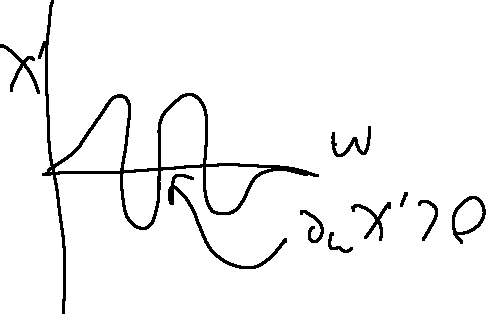
\includegraphics[width=10cm]{images/11-26-1.png}
	\caption*{Plot of 3LS $\chi'$}
\end{figure*}
Using this formula, when the slope becomes very high we will have light that has a group velocity much much slower than normal (as slow as 10m/s).
How do we understand this? We can think of this as the adiabatic passage of a dark state. If we start in the dark state, and send in a probe pulse then we will see our population remain in the dark state *which begins as $\ket{1}$.
\begin{figure*}[h!]
	\centering
	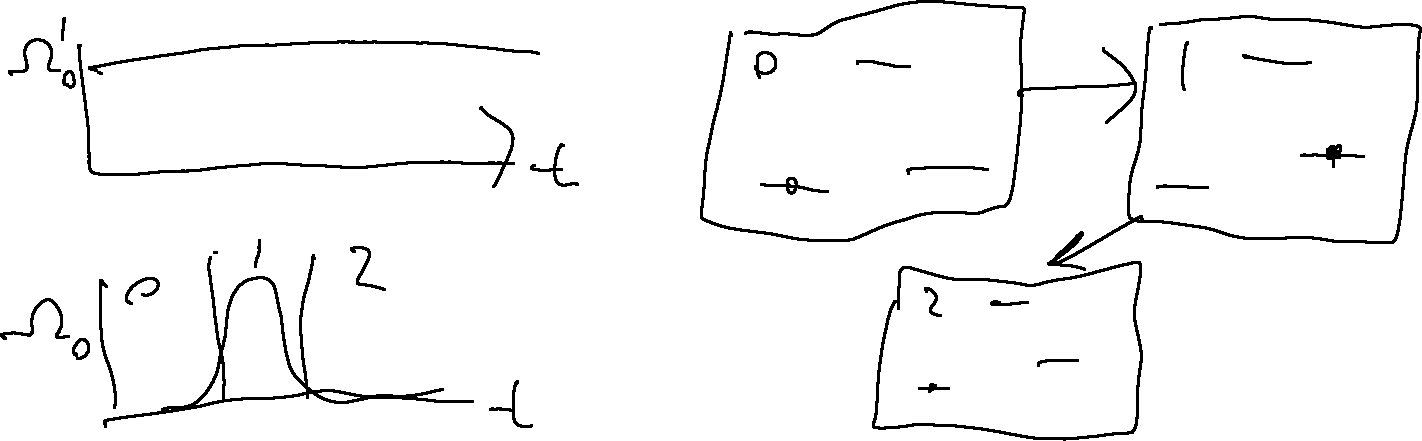
\includegraphics[width=10cm]{images/11-26-2.png} \\
	\caption*{Plot of the state as a pulsed probe is incident on the sample}
\end{figure*}
Once the probe arrives we see the population move to three, and then back to one as the pulse leaves.

Looking at the field we see this as an energy exchange. First we put energy from the field into the state for the transition from $\ket{1}\to\ket{3}$. Then we take energy out of the state and put it back into the field going from $\ket{3}\to\ket{1}$.
The rate of energy exchange is $~\Omega_0'$, so our group velocity scales with $\Omega_0'$. It can be shown that $v_g\propto\Omega_0'\ ^2$. This can be used to store light. If $\alpha L \gg 1$ then the probe is completely absorbed by the medium.
After this our $\rho_{13}$ is not zero. Not only not this value contains the information of the probe pulse. Therefore we say the probe pulse is stored in the medium as the coherence.

We want to know how to retrieve this information. In order to do this we simply need to apply a pump field to our sample.
\begin{figure*}[h!]
	\centering
	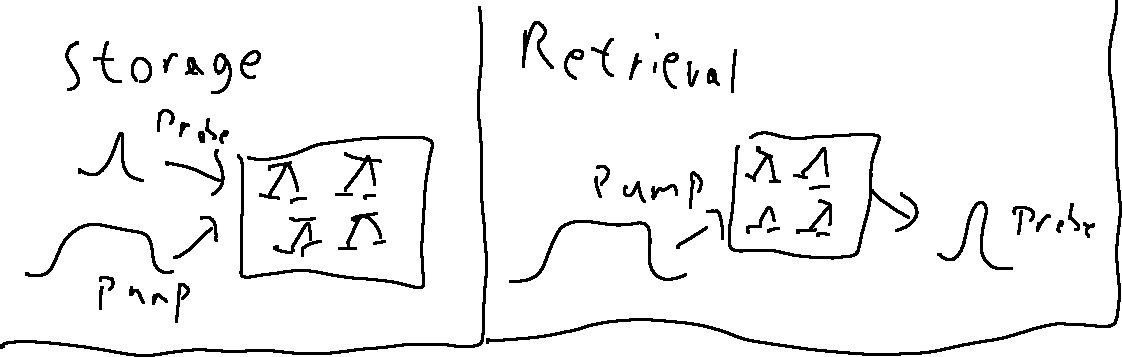
\includegraphics[width=10cm]{images/11-26-3.png}
	\caption*{Storage and retrieval of an optical field}
\end{figure*}
\subsection{Summary}
We introduced the idea of dark states, and used this idea to introduce the phenomena of coherent population trapping (related to $\rho_{22}$) and electromagnetically induced transparency (related to $\chi$).
Using adiabatic passage we also could see STIRAP, slow light and light storage. In all these our nonradiative coherence $\rho_{13}$ plays a central role.

Additionally we can see that for other types of three level systems (V or cascade). In both of these systems our $\rho_{13}$ decays via spontaneous emission, so it is shorter lived and these techniques aren't as powerful.
Finally we can look at EIT as a result of classical coupled harmonic oscilators.
\section{Mechanical effects of light}
\subsection{Overview}
The key insight of this section will be that light carries momentum (you can see this in Maxwell's equations).
In quantum mechanics we know that the momentum of a photon is $\hbar\bm{k}$. Therefore optical interactions must satisfy momentum conservation. The force applied is typcially quite small in macroscopic scales (~1W lasers will apply ~1nN of force).
Looking at the interaction of an atom with a photon instead, we see that not only will the atom's state change, but so will it's momentum, i.e. the change will be $\Delta\bm{p} = \hbar\bm{k}$, similarly for emission $\Delta\bm{p} = -\hbar\bm{k}$,
where in both of these $\bm{k}$ is the photon's wave vector.
\begin{figure*}[h!]
	\centering
	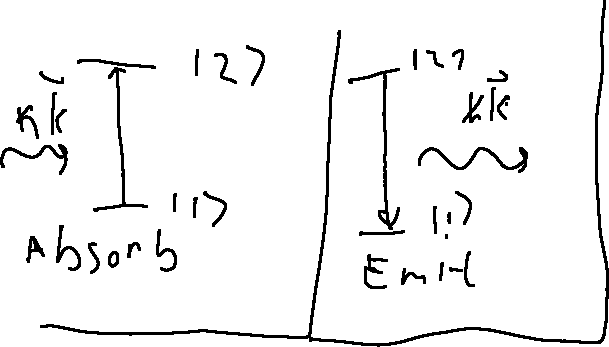
\includegraphics[width=10cm]{images/11-26-4.png}
	\caption*{Change in momentum from Emision and Absorption}
\end{figure*}
\subsection{Radiation Pressure}
This is sometimes called dissipative force. 

We start by ignoring spontatneous emission. This process will be absorption followed by stimulated emission, and since the wave vector will be the same for the absorbed and emitted light, then the overall change in momentum is zero.

\begin{figure*}[h!]
	\centering
	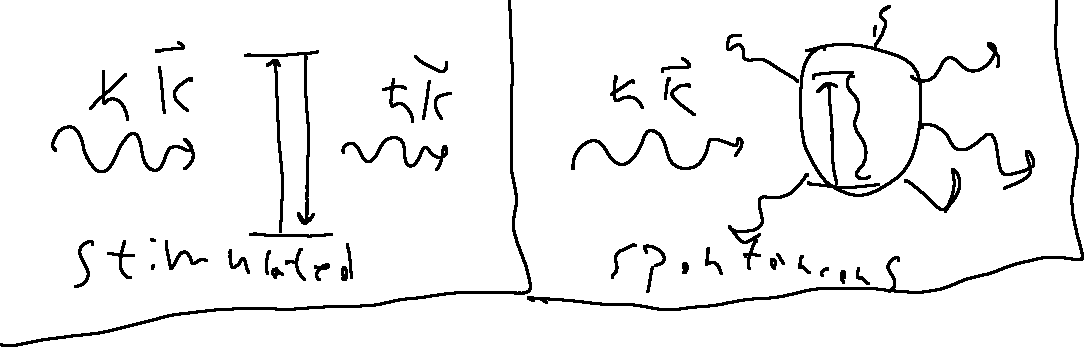
\includegraphics[width=10cm]{images/11-26-5.png}
	\caption*{Change in momentum from Stimulated and Spontaneous emission}
\end{figure*}

If we instead include the stimulated emission process, then we have $\hbar\bm{k}$ absorbed, and the $\hbar\bm{k}'$ emitted, where $\bm{k}'$ is the same magnitude as $\bm{k}$ but points in a random direction. On average the momentum change from the emission is zero,
therefore the total momentum change is going to be $\hbar\bm{k}$. If we continously shine a laser on a sample that will spontaneously emit photons, then the total change will be $\hbar\bm{k}\gamma_2\rho_{22}\Delta t$.
Therefore the force will be:
\begin{align*}
	\bm{F} &= \frac{\expval{\Delta \bm{p}}}{\Delta t} \\
	\bm{F} &= \hbar\bm{k}\gamma_2\rho_{22} \\
	\bm{F} &= \hbar\bm{k}\gamma_2\frac{\Omega_0|^2\gamma}{2\gamma_2}\frac{1}{\delta^2 + \gamma^2}
\end{align*}
And clearly the maximum force must be (because in steady state $\rho_{22} \leq \frac{1}{2}$):
\begin{align*}
	\bm{F}_\text{max} &= \frac{1}{2}\hbar\bm{k}\gamma_2
\end{align*}
\subsection{Doppler cooling}
We start by briefly reviewing the Doppler shift. If we look at an atom moving with a velocity $v$, we can say energy and momentum conservation together yield:
\begin{align*}
	m\bm{v} + \hbar\bm{k} &= m\bm{v}' \\
	\frac{1}{2}mv^2 + \hbar\omega_1 + \hbar \omega &= \hbar\omega_2 + \frac{1}{2}mv'\ ^2 \\
	\frac{1}{2}mv^2 + \hbar\omega_1 + \hbar \omega &= \hbar\omega_2 + \frac{1}{2m} (m\bm{v} + \hbar \bm{k})^2 \\
	\frac{1}{2}mv^2 + \hbar\omega_1 + \hbar \omega &= \hbar\omega_2 + \frac{1}{2}mv^2 +\frac{1}{2m} \hbar^2k^2 + \frac{1}{2}m\hbar\bm{v}\cdot\bm{k} \\
	\hbar\omega_1 + \hbar \omega &= \hbar\omega_2 +\frac{1}{2m} \hbar^2k^2 + \frac{1}{2}m\hbar\bm{v}\cdot\bm{k}
\end{align*}
Looking at $\frac{1}{2m} \hbar^2k^2$ we can see that this term will be very small, since $k$ is much smaller (when using equivalent units) than $m$, so:
\begin{align*}
	\omega_2 - \omega_1 &= \omega - \bm{k}\cdot\bm{v}
\end{align*}
So our resonance condition becomes $\omega_0 = \omega - \bm{k}\cdot\bm{v}$ where this shift to resonance is known as the Doppler shift.

If we choose our $\bm{k}$ along $\bm{v}$ then $\omega_0 = \omega - kv$, so the frequency of the light we send in is effectively down shifted (we need to use a higher frequency laser to drive the transition).

If instead we use $\bm{k}$ antiparallel to $\bm{v}$ then $\omega_0 = \omega + kv$, so the light we send in is effectively up shifted (we need a lower frequency laser to drive the transition).

\begin{figure*}[h!]
	\centering
	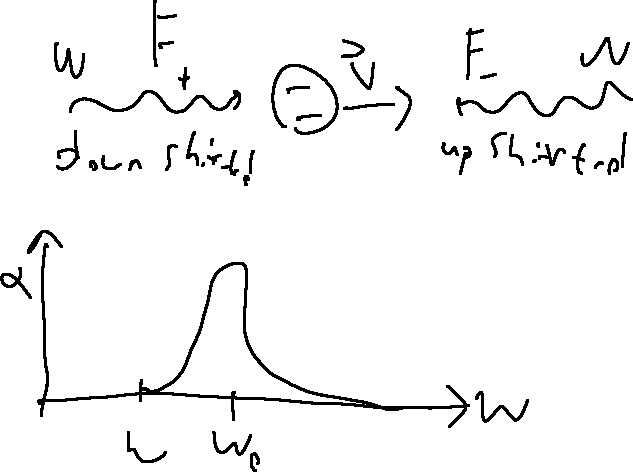
\includegraphics[width=10cm]{images/11-26-6.png}
	\caption*{Doppler cooling}
\end{figure*}
For doppler cooling we have two optical fields incident on an atom in opposite directions. By choosing $\omega$ less than $\omega_0$ we cause the force applied by the laser in the opposite direction of the motion to be greater than the one in the direction of motion.
This leads to a cooling/fricitional force/cooling force. We will eventually show $F\propto v$.

The exact (average) force we find for a moving particle is:
\begin{align*}
	F &= \frac{1}{2}\hbar k |\Omega_0|^2 \frac{\gamma}{(\omega_0 - \omega + \bm{k}\cdot\bm{v})^2 + \gamma'\ ^2}
\end{align*}
We now seek to calculate the net force applied by a our two lasers that are incident from different directiions:
\begin{align*}
	F_+ &= \frac{1}{2}\hbar k |\Omega_0|^2 \frac{\gamma}{(\omega_0 - \omega + kv)^2 + \gamma'\ ^2} \\
	F_- &= -\frac{1}{2}\hbar k |\Omega_0|^2 \frac{\gamma}{(\omega_0 - \omega - kv)^2 + \gamma'\ ^2}
\end{align*}
We now assume that the detuning is much greater than the doppler shift $|\omega - \omega_0| \gg kv$, so $(\omega_0 - \omega \pm kv)^2 \approx \delta^2 \pm 2\delta kv$. Therefore:
\begin{align*}
	F_\pm &= \pm\frac{1}{2}\hbar k |\Omega_0|^2 \frac{\gamma}{\delta^2 + \gamma'\ ^2}\frac{1}{1\pm \frac{2\delta kv}{\delta^2 + \gamma'\ ^2}} \\
	F_\pm &= \pm\frac{1}{2}\hbar k |\Omega_0|^2 \frac{\gamma}{\delta^2 + \gamma'\ ^2}\left(1\mp \frac{2\delta kv}{\delta^2 + \gamma'\ ^2}\right) \\
	F_\pm &= \pm F_0 - \frac{1}{2}\beta v
\end{align*}
Where:
\begin{align*}
	\beta &= 2\hbar k^2|\Omega_0|^2 \frac{\gamma}{(\delta^2 + \gamma'\ ^2)^2} \delta &
	F_0 &= \frac{1}{2}\hbar k |\Omega_0|^2 \frac{\gamma}{\delta^2 + \gamma'\ ^2}
\end{align*}
So our net force is then:
\begin{align*}
	F &= F_+ + F_- \\
	F &= -\beta v
\end{align*}
So we see we have a damping force. Additionally in practical experiments, as the atom cools, we would decrease the detuning to increase the effect of doppler cooling.

We now naturally wonder how cool can our Doppler cooling get. The key to understanding this is to understand what heating process counterbalances our cooling.
In fact the spontaneous emission process involves a random recoil, despite the fact it is our primary cooling process, it will also be our heating process.
In theremal equilibrium we know our heating and cooling rates will be equal. Our heating rate will be $\frac{(\hbar k)^2}{2M} \rho_{22}\gamma_2$, while the cooling rate is $\expval{\beta v^2}$. So in equilibrium:
\begin{align*}
	\frac{(\hbar k)^2}{2M} \rho_{22} \gamma_2 &= \expval{\beta v^2} \\
	\frac{(\hbar k)^2}{2M} \rho_{22} \gamma_2 &= \beta \frac{k_B T}{M} \\
	\frac{(\hbar k)^2}{2} \rho_{22} \gamma_2 &= \beta k_B T \\
	\frac{(\hbar k)^2}{2} \gamma_2 \frac{|\Omega_0|^2 \gamma}{\gamma_2(\delta^2 + \gamma'\ ^2)} &= k_B T 2\hbar k^2 \frac{|\Omega_0|^2 \gamma \delta}{(\delta^2 +\gamma'\ ^2)^2} \\
	k_B T &= \frac{\hbar}{4} \frac{\delta^2 + \gamma'\ ^2}{\delta} \\
	k_B T &= \frac{\hbar\gamma'}{2} \frac{\delta^2 + \gamma'\ ^2}{2|\delta|\gamma'}
\end{align*}
So:
\begin{align*}
	k_B T &> \frac{\hbar\gamma'}{2} \\
	T_D &= \frac{\hbar\gamma'}{2k_B}
\end{align*}
When first trying to verify this, experiments with $T_D \approx 170 \mu K$ yielded a temperature with $40 \mu K$! This was seen by multiple experiments, and took nearly a year to understand. The explination will be covered in the next lecture.

We already have a cooling force, but we also need to have a trapping force to keep the atoms in place. This can be done with a magneto optic trap.
\subsection{Another perspective}
We have so far looked at these mechanical effects from the perspective of momentum conservation. We ill now look at this from the perspective of dispersive, gradient and dipole forces. Starting from our interaction Hamiltonian:
\begin{align*}
	V &= -\bm{\mu}\cdot\bm{E} &
	\hat{\bm{F}} &= \partial_t \bm{p} \\
	\hat{\bm{F}} &= \frac{1}{i\hbar} [\bm{p}, V] &
	\hat{\bm{F}} &= -\del V
\end{align*}
So our average force is:
\begin{align*}
	\bm{F} &= \expval{\hat{\bm{F}}} \\
	\bm{F} &= -\expval{\del V}
\end{align*}
We now quickly express our potential explicitly:
\begin{align*}
	V &= \frac{\hbar}{2}\Omega_0\sigma_+ + \text{h.c.} &
	\sigma_+ &= \ket{2}\bra{1} \\
	\Omega_0(\bm{r}) &= -\frac{\mu E(\bm{r})}{\hbar} e^{i\phi(\bm{r})} & 
	\Omega_0(\bm{r}) &= |\Omega_0(\bm{r})|e^{i\phi(\bm{r})}
\end{align*}
So:
\begin{align*}
	F &= -\frac{\hbar}{2}\del \Omega_0\expval{\sigma_+} + \text{c.c.} \\
	\expval{\sigma_+} &= \rho_{12} \\
	\expval{\sigma_+} &= -\frac{\Omega_0^*}{2} \frac{1}{\delta + i\gamma} \frac{\delta^2 + \gamma^2}{\delta^2 + \gamma'\ ^2} \\
	\del \Omega_0 &= e^{i\phi}\del |\Omega_0| + i|\Omega_0| e^{i\phi} \del \phi \\
	\del \Omega_0 &= \Omega_0 \left(\frac{\del|\Omega_0|}{|\Omega_0|} + i\del\phi\right) \\
	\bm{F} &= \frac{\hbar}{4}|\Omega_0|^2 \frac{1}{\delta + i\gamma}\frac{\delta^2 + \gamma^2}{\delta^2 + \gamma'\ ^2} \left(\frac{\del|\Omega_0|}{|\Omega_0|} + i\del\phi\right) + \text{c.c.} \\
	\bm{F} &= \frac{\hbar}{4}|\Omega_0|^2 \frac{\delta^2 + \gamma^2}{\delta^2 + \gamma'\ ^2}\left(\frac{-i\gamma}{\delta^2 + \gamma^2} + \frac{\delta}{\delta^2 + \gamma^2}\right) \left(\frac{\del|\Omega_0|}{|\Omega_0|} + i\del\phi\right) + \text{c.c.} \\
	\bm{F} &= \frac{\hbar}{2}|\Omega_0|^2 \frac{\delta^2 + \gamma^2}{\delta^2 + \gamma'\ ^2}\left(\frac{\gamma}{\delta^2 + \gamma^2} \del\phi + \frac{\delta}{\delta^2 + \gamma^2} \frac{\del|\Omega_0|}{|\Omega_0|}\right) \\
	\bm{F} &= \frac{\hbar}{2}|\Omega_0|^2 \frac{1}{\delta^2 + \gamma'\ ^2}\left(\gamma\del\phi + \delta\frac{\del|\Omega_0|}{|\Omega_0|}\right)
\end{align*}
This force has two components, a dissipative force related to $\del\phi$ and a dispersive force related to $\del|\Omega_0|$.
\begin{align*}
	\bm{F}_\text{diss} &= \frac{\hbar}{2}|\Omega_0|^2 \frac{\gamma}{\delta^2 + \gamma'\ ^2}\del\phi \\
	\bm{F}_\text{disp} &= \frac{\hbar}{2}|\Omega_0|^2 \frac{\delta}{\delta^2 + \gamma'\ ^2}\frac{\del|\Omega_0|}{|\Omega_0|} \\
	\bm{F}_\text{disp} &= \frac{\hbar}{4} \frac{\delta}{\delta^2 + \gamma'\ ^2}\del |\Omega_0|^2
\end{align*}
We know for a plane wave $\del|\Omega_0| = 0$ and $\del\phi = \bm{k}$, so for a plane wave:
\begin{align*}
	\bm{F} &= \frac{\hbar}{2}\bm{k} |\Omega_0|^2 \frac{\gamma}{\delta^2 + \gamma'\ ^2}
\end{align*}
Which is what we derived before, so our dissipative force is the force we found for spontaneous emission/absorption.

If we work with a beam of spoot size $~a$, then we will have:
\begin{align*}
	\bm{F}_\text{disp} &\approx \frac{\hbar}{4} \frac{\delta}{\delta^2 + \gamma'\ ^2}\frac{|\Omega_0|^2}{a}
\end{align*}
If we instead look at writing our force in terms of a potential we can say that:
\begin{align*}
	\bm{F}_\text{disp} &= \frac{\hbar}{4} \frac{\delta}{\delta^2 + \gamma^2 + \frac{|\Omega_0|^2}{2}}\del |\Omega_0|^2 \\
	\bm{F}_\text{disp} &= - \del V_\text{opt} \\
	V_\text{opt} &= -\frac{\hbar\delta}{2}\ln \left(1 + \frac{1}{2}\frac{|\Omega_0|^2}{\delta^2 + \gamma^2}\right)
\end{align*}
If we are far off resonance, $\delta \gg \gamma_3$ and $\delta \gg \Omega_0$, then:
\begin{align*}
	V_\text{opt} &\approx -\frac{\hbar\delta}{2}\frac{1}{2}\frac{|\Omega_0|^2}{\delta^2} \\
	V_\text{opt} &\approx -\frac{\hbar}{4}\frac{|\Omega_0|^2}{\delta}
\end{align*}
Which is the optical stark shift. This can be used to create optical tweezers which hold particles in place using a spatially varying intensity.
Additionaly, this can be used to create an optical latice with a periodic potential, where atoms are trapped in one of many potential wells.
\begin{figure*}[h!]
	\centering
	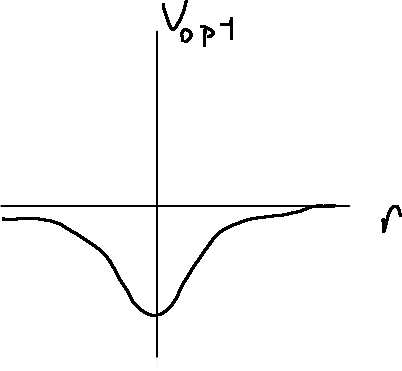
\includegraphics[width=10cm]{images/12-03-1.png}
	\caption*{Potential for Optical tweezers}
\end{figure*}
\begin{figure*}[h!]
	\centering
	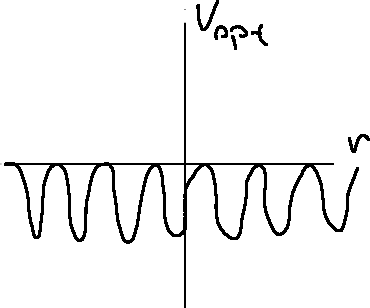
\includegraphics[width=10cm]{images/12-03-2.png}
	\caption*{Potential for Optical lattice}
\end{figure*}
Can we understand the optical stark shift now in terms of conservation of momentum? If our incoming wave is not a plane wave, then we have many wave vectors associated with our beam $\bm{k}$.
If we absorb and re-emit according to different $\bm{k}$s from our beam, then (after some math that is out of scope for what we are looking at), we will see the optical stark shift!

\subsection{Sub-Doppler cooling}
It is possible that the cooling below the doppler limit could be caused by a gradient force in the laser intensity.
Typically we expect to see our two laser fields with identical polarization, so they will form spatially standing waves.
If we make these polarizations orthogonal, there will be no spatial intensity modulation which surprisingly gives better results.
So this doesn't really seem to explain how we broke the doppler limit.

We next consider the additional energy levels of the atom, instead of looking at it as a two level system, we consider a hyperfinely split system (which has many energy levels).

We could also consider if there is a polarization gradient. If we have two conterporpogating fields with different polarizations then you find that the net polarization is circular:
\begin{align*}
	\bm{E}_l &= E_0\hat{e}_x e^{ikz} \\
	\bm{E}_r &= E_0\hat{e}_y e^{-ikz} \\
	\bm{E} &= \bm{E}_l + \bm{E}_r & \text{Assuming out of face for simplicity} \\
	\bm{E} &\propto (\hat{e}_x + i\hat{e}_y)\cos kz + i(\hat{e}_x - i\hat{e}_y)\sin kz \\
	\bm{E} &\propto \hat{e}_+\cos kz + i\hat{e}_y\sin kz
\end{align*}
Which are circularly polarized waves, with the portion of each polarization varying spatially. These two different polarizations cause our system to couple to multiple states.
The process of optical pumping then governs a dissipative process using these mechanisms.

To fully charactorize this process we would need to look at Clebsch-Gordon coefficients for different transitions, but instead here we approach this with a simplified model.
We consider in our model the $J=\frac{1}{2}\to J=\frac{1}{2}$ transition. 
\begin{figure*}[h!]
	\centering
	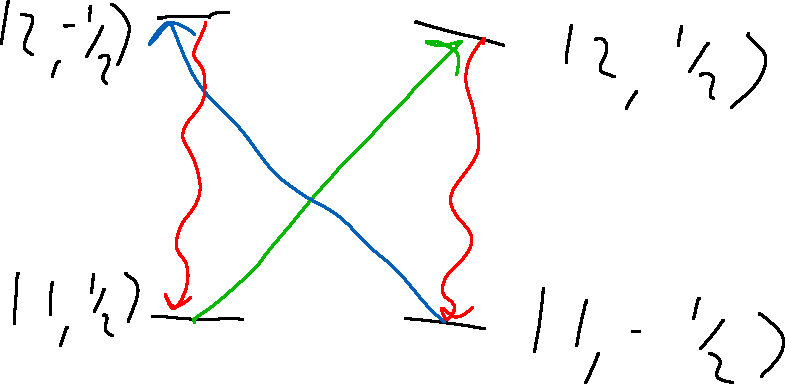
\includegraphics[width=10cm]{images/12-05-1.png}
	\caption*{Transitions for our model, in green is the $\sigma_+$ transition, in blue is the $\sigma_-$ transition and in red is the optical pumping transition}
\end{figure*}
As the atoms move around they reach the peak of their corresponding potentials due to the polarizations coopling to the other states.
At the peak they are most likely to be excited to a higher state, which then decays to a lower state that couples via the opposite polarization of light.
Therefore the atom finds itself at the bototom of a well, then they repeat this proces, losing $\frac{\hbar|\Omega_0|^2}{4|\delta|}$.
\begin{figure*}[h!]
	\centering
	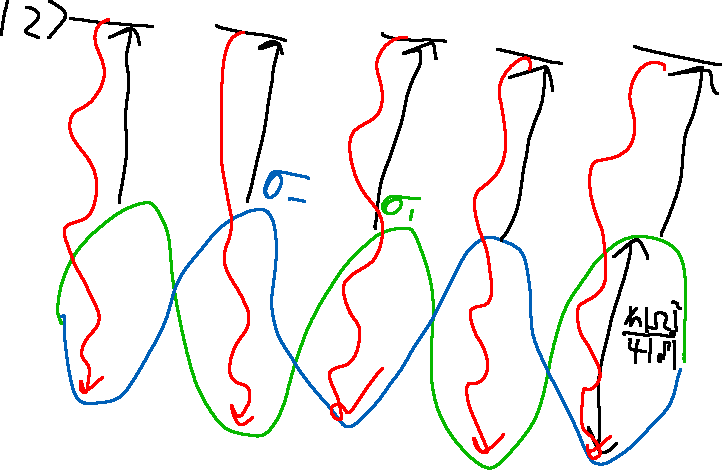
\includegraphics[width=10cm]{images/12-05-2.png}
	\caption*{Atoms in sysyphus cooling potential}
\end{figure*}
This process works well when $k_B T > \frac{\hbar |\Omega_0|^2}{4|\delta|}$. Additionally we have a recoil limit $\frac{(\hbar k)^2}{2M} = k_B T_r$.
This recoil limit is $T_R~1\mu K$.

Now we clearly want to concider how to circumvent this cooling limit. In order to do this we want to avoid spontaneous emission, and therefore avoid the excited state whenever possible.
In orer to avoid exciting the atom we utilize the dark state.

When we include the momentum in our state, we have the dark and bright states (when the fields are equal) are described by:
\begin{align*}
	\ket{D,p} &= \frac{1}{\sqrt{2}}(\ket{+1,p+\hbar k} - \ket{-1,p-\hbar k}) \\
	\ket{B,p} &= \frac{1}{\sqrt{2}}(\ket{+1,p+\hbar k} + \ket{-1,p-\hbar k})
\end{align*}
\begin{figure*}[h!]
	\centering
	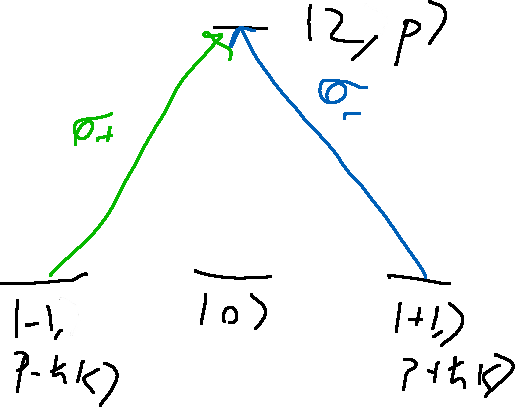
\includegraphics[width=10cm]{images/12-05-3.png}
	\caption*{Dark states in our sysyphus cooling setup}
\end{figure*}
We see that the $\ket{D,p}$ state is only dark if $p=0$. This allows for cooling because any state can be randomly put into $\ket{D,p}$ by random recoil, which will then stay in that state for all time since it is a dark state.
This is known as velocity selective CPT.

In trapped ions there is also the process of resolved sideband cooling.

\chapter{Winter Term, Brian Smith}
\section{Review}
\subsection{Classical Mechanics}
We can look at classical mechanics in terms of three different formalizims, all of these describe how classical particles move in space.

The first is the Newtonian model in which we describe things in terms of forces applied, i.e. $\sum\bm{F}  = m\ddot{\bm{x}}$.
As an example, take a particle moving with mass m in 1 dimension with an arbitrary potential, so:
\begin{align*}
	F &= -\partder{V}{x} \\
	m\ddot{x} &= -\partder{V}{x}
\end{align*}

The second is the Lagrangian formulation in which $L = T -V$, the equations of motion determined from $\delta S = 0$ where $S = \int L dt$. In other words this turns our problem into a variational calculus  problem.
\begin{align*}
	\delta S  &= \int \left(\partder{L}{q} \delta q + \partder{L}{\dot{q}} \delta \dot{q}\right) dt \\
	\delta S  &= \int \left(\partder{L}{q} \delta q - \frac{d}{dt}\partder{L}{\dot{q}} \delta q\right) dt \\
	\delta S  &= \int \left(\partder{L}{q}  - \frac{d}{dt}\partder{L}{\dot{q}}\right)\delta q dt \\
	\partial_q L &= \frac{d}{dt}\partder{L}{\dot{q}}
\end{align*}

As an example, take a particle moving with mass m in 1 dimension with an arbitrary potential, so:
\begin{align*}
	L &= \frac{m}{2}\dot{x}^2 - V(x) \\
	\partder{L}{x} &= -\partder{V}{x} \\
	\partder{L}{{\dot{x}}} &= m \dot{x} & \text{We call this term the conjugate momentum } p_x\\
	m \ddot{x} &= -\partder{V}{x}
\end{align*}
So here we see the result matches what we saw for Newtonian mechanics.

The third is the Hamiltonian formulation in which $H = \sum p_i \dot{q}_i - L$ (the legendre transform of the Lagrangian formulations). Here we first determine our conjugate momenta $p_j = \partder{L}{\dot{q}_j}$.
Then we construct $H = p_j \dot{q}_j - L$. Now we minimize the action again in terms of $q_j$ and $p_j$, but that is unweildy, so:
\begin{align*}
	\partder{H}{q} &= -\partder{q}{L} - \partder{L}{\dot{q}} \partder{\dot{q}}{q} + \partder{}{q} (p \dot{q}) \\
	\partder{H}{q} &= -\partder{q}{L} - \partder{L}{\dot{q}} \partder{\dot{q}}{q} + \partder{p}{q} \dot{q} + \partder{\dot{q}}{q} p \\
	\partder{H}{q} &= -\partder{q}{L} - \partder{L}{\dot{q}} \partder{\dot{q}}{q} + \partder{\dot{q}}{q} p \\
	\partder{H}{q} &= -\partder{L}{q} \\
	\partder{H}{q} &= -\dot{p}
\end{align*}
We now look at our other equation of motion:
\begin{align*}
	\partder{H}{p} &= \partder{}{p} (p\dot{q}) - \partder{L}{p} \\
	\partder{H}{p} &= \dot{q}
\end{align*}
Looking again at a particle with mass m in 1 dimension with an arbitrary potential:
\begin{align*}
	p &= m\dot{x} \\
	H &= p\dot{x} - L \\
	H &= \frac{p^2}{m} - \frac{p^2}{2m} + V(x) \\ 
	H &= \frac{p^2}{2m}  + V(x) \\
	\dot{x} &= \frac{p}{m} \\
	-\dot{p} &= \partder{V}{x} \\
	\ddot{x} &= \frac{\dot{p}}{m} \\
	m\ddot{x} &= -\partder{V}{x}
\end{align*}
Which again matches the Newtonian approach.

Alternatively we could use the Poisson formalism. We say the Poisson bracket is defined:
\begin{align*}
	\{f,g\} &= \sum_i \partder{f}{q_i}\partder{g}{p_i} - \partder{g}{q_i}\partder{f}{p_i}
\end{align*}

We can see that for any quantity:
\begin{align*}
	\{f,H\} &= \dot{f}
\end{align*}

If we now look at the motion of a pendulum:\\ 
\includegraphics*[width=8cm]{images/1-06-fig1.png} \\
We can quickly derive that:
\begin{align*}
	q &= l\theta \\
	V &= mgy \\
	p &= m\dot{\theta} \\
	\omega &= \frac{g}{q} \\
	H &= \frac{1}{2m} p^2 + \frac{m}{2} \omega q^2
\end{align*}

If we want to quantize a system we do two things: \\
0) Determine $H$, $p$ and $q$ for our classical system, such that the Hamilton equations of motion give correct classical dynamics. These must be canonically conjugate variables such that $p_i = \partder{L}{\dot{q}_i}$. \\
1) We then determine the Poisson brackets for $q_i$ and $p_i$. \\
2) We then change our canonically conjugate variables to operators acting on a Hilbert space, with commutators given by $[\hat{a},\hat{b}] = i\hbar\{a,b\}$

Now to quantize our pendulum:
\begin{align*}
	\hat{H} &= \frac{\hat{p}^2}{2m} + \frac{m\omega^2}{2}\hat{q}^2
\end{align*}
To solve this we use ladder/creation/raising/anihilation/lowering operators:
\begin{align*}
	\hat{a}^\dagger &= \sqrt{\frac{mw}{2\hbar}} \left(\hat{q} - \frac{i}{m\omega} \hat{p}\right) \\
	\hat{a} &= \sqrt{\frac{mw}{2\hbar}} \left(\hat{q} + \frac{i}{m\omega} \hat{p}\right)
\end{align*}
These operators are non-Hermition, and therefore they can't represent an observable. If we say we have energy eigenstates $\hat{H}\ket{\psi} = E\ket{\psi}$, we claim that $\hat{H}\hat{a}^\dagger \ket{\psi} = (E + \hbar\omega)\ket{\psi}$.
In order to show this we rewrite our Hamiltonian:
\begin{align*}
	\hat{q} &= \sqrt{\frac{2\hbar}{m\omega}} \frac{\hat{a} + \hat{a}^\dagger}{2} \\
	\hat{p} &= \sqrt{\frac{2\hbar}{m\omega}} m\omega\frac{\hat{a} - \hat{a}^\dagger}{2i}
\end{align*}

\section{Field Quantization}
There are two standard approaches to field quantization:\\\\
1) The standard approach (for high energy physics, Condensced matter theory (in which we would instead have an effective field theory)) involves writing down a Lagrangian density/Action in terms of a density:
\begin{align*}
	S &= \int dt L(\phi(\bm{x},t),\partial_\mu \phi(\bm{x},t),t) \\
	S &= \int dt d^3 x \mathcal{L}(\phi(\bm{x},t),\partial_\mu \phi(\bm{x},t),t)
\end{align*}
Which allows you to determine the equations of motion for classical fields. If you follow this procedure for a scalar field of mass $m$, then you end up finding a lagrange density:
\begin{align*}
	\mathcal{L} &= (\partial_\mu\phi)(\partial^\mu\phi) - m^2\phi^2 \\
	(-i\hbar\partial_t)^2\phi + c^2 (i\hbar\del)^2\phi &= m^2c^4\phi
\end{align*}
When we move towards a more complete theory of quantum mechanics, we realize that there are no particles, and rather all interactions are done by quantum fields, where the things we describe as particles are in fact excitations of quantum fields.
We will see that a photon is an excitation of the electromagnetic field that occupies a specific mode of the EM field.

Once we have our classical equations of motion here, we ``Raise'' fields and conjugate momenta into operators, and impose commutators:
\begin{align*}
	\hat{\phi}(\bm{x},t),&& \hat{\pi}(\bm{x},t) &= \partder{\mathcal{L}}{\dot{\phi}} \\
	[\hat{\phi}(\bm{x},t),\hat{\pi}(\bm{x}',t)] &= i\hbar\delta(\bm{x} - \bm{x}')
\end{align*}
(This is correct for scalar fields, and massive vector fields, but must be modified for spinor fields and massless vector fields)
\\\\
2) We will now start our approach with a review of classical Electromagnetism:
\subsection{Review of Classical Electromagnetism}
We start with Maxwell's equation:
\begin{align*}
	\del\cdot\bm{B} &=0 & \del\cdot\bm{E} &+ \frac{\rho}{\epsilon_0} \\
	\del\times\bm{B} &= \mu_0\bm{j} + \mu_0\epsilon_0\partial_t \bm{E} &
	\del\times\bm{E} &= - \partial_t \bm{E} \\
	\bm{H} &= \frac{1}{\mu_0} \bm{B} - \bm{M} &
	\bm{D} &= \epsilon_0\bm{E} + \bm{P}
\end{align*}
and the Lorentz force law:
\begin{align*}
	\bm{F} &= q(\bm{E} + \bm{v}\times\bm{B})
\end{align*}
We can define the Hamiltonian(energy for free fields) and the Lagrangian:
\begin{align*}
	H &= \int d^3x \frac{\epsilon_0}{2}\left[\bm{E}^2 + c^2\bm{B}^2\right] \\
	L &= \int d^3x \frac{\epsilon_0}{2}\left[\bm{E}^2 - c^2 \bm{B}^2\right]
\end{align*}
Where here we are looking at in vacua fields. We also have a pointing vector:
\begin{align*}
	\bm{S} &= \frac{1}{\mu_0}\bm{E}\cross\bm{B} \\
	\bm{P} &= \int d^3 x \bm{S} \\
	\bm{J} &= \frac{1}{\mu_0}\int d^3 x\bm{x} \cross (\bm{E}\cross\bm{B})
\end{align*}
Where $\bm{P}$ is linear momentum, and $\bm{J}$ is angular momentum. Finally we introduce scalar and vector potentials:
\begin{align*}
	\bm{B} &= \del\times\bm{A} \\
	\bm{E} &= -\del\phi - \partial_t \bm{A}
\end{align*}
These potentials imply:
\begin{align*}
	\del\cdot\bm{B} &= 0 &
	\del\cross\bm{E} &= -\partial_t \bm{B}
\end{align*}
These fields are invarient under the gauge transformation:
\begin{align*}
	\phi' &= \phi - \partial_t \chi \\
	\bm{A}' &= \bm{A} +\del\chi
\end{align*}
And commonly we choose to either use the Lorentz gauge:
\begin{align*}
	\del\cdot\bm{A} &= \frac{1}{c^2} \partial_t\phi
\end{align*}
Which lets us then construct $A_\mu = (\phi/c,\bm{A})$ and $\partial_\mu =(\partial_t/c,\del)$, so we can then say $\partial_\mu A^\mu$ is a Lorentz scalar. 

Or instead (which is the choice we will use in classical Electromagnetism) we can choose the Radiation or Coulomb Gauge:
\begin{align*}
	\del\cdot\bm{A} &= 0
\end{align*}
Which immediately implies:
\begin{align*}
	\phi(\bm{x},t) &= \frac{1}{4\pi\epsilon_0}\int d^3x' \frac{\rho(\bm{x}',t)}{|\bm{x} - \bm{x'}|}
\end{align*}
If we are in the free field ($\rho = 0$, $\bm{j} = 0$):
\begin{align*}
	\del\cdot\bm{E} &= \del\cdot(-\del\phi - \partial_t\bm{A}) \\
	\nabla^2\phi &= 0
\end{align*}
And:
\begin{align*}
	\del\times\bm{B} &= \del\cross\del\cross\bm{A} \\
	\del\times\bm{B} &= -\nabla^2\bm{A} \\
	(\nabla^2 -\frac{1}{c^2}\partial_t^2)\bm{A} &= 0
\end{align*}
So in the Coulomb gauge we see that the vector potential obeys the wave equation. Additionally $\bm{A}$ will be a transverse field, so the direction of propogation is perpendicular to the field itself.
Although this choice of gauge is not manifestly Lorentz invariant, i.e. the quantities change in different fields of reference, but we still see that our theory will obey relativity.
Additionally since in quantum optics we typically don't deal with frames that are related to eachother by relativistic speeds, we don't need to worry about maintaining exact Lorentz invariants here.

We now consider a free field in a cube of side $L$:

We start by expanding the classical EM field into a set of orthonormal modes. Where each individual mode is a solution to Maxwell's equations (in a particular geometry/ source configuration).
Here we choose to use plane waves as our modes, so:
\begin{align*}
	\bm{E} (\bm{x},t) &= \sum_{\bm{n}} \tilde{\bm{E}}_{\bm{n}}(t) e^{i\bm{k}_{\bm{n}}\cdot\bm{x}} + \compcon \\
	\bm{k}_{\bm{n}} &= (n_x,n_y,n_z) \frac{2\pi}{L}
\end{align*}
These are equivalent to imposing periodic boundry conditions on the edge of the box. For a general problem, we can take $L$ to $\infty$ to include the entire universe. Similarly we find:
\begin{align*}
	\bm{B}(\bm{x},t) &= \sum_{\bm{n}} \tilde{\bm{B}}_{\bm{n}}(t) e_{i\bm{k}_{\bm{n}} \cdot\bm{x}} + \compcon \\
	\bm{A}(\bm{x},t) &= \sum_{\bm{n}} \tilde{\bm{A}}_{\bm{n}}(t) e_{i\bm{k}_{\bm{n}} \cdot\bm{x}} + \compcon
\end{align*}
We can see that these must all be real valued fields, so $\tilde{\bm{E}}_{\bm{n}}^* = \tilde{\bm{E}}_{-\bm{n}}$, and also the same will be true for $\tilde{\bm{B}}_{\bm{n}}$ and $\tilde{\bm{A}}_{\bm{n}}$.

From:
\begin{align*}
	\del\cdot\bm{B} &= 0 &
	\del\cdot\bm{E} &= 0 &
	\del\cdot\bm{E} &= 0
\end{align*}
We know that:
\begin{align*}
	\del\cdot\bm{F} (\bm{x},t) &= \sum_{\bm{n}} \del\cdot\left((\tilde{\bm{F}}_{\bm{n}}(t) e^{i\bm{k}_{\bm{n}}\cdot\bm{x}} + \compcon\right) \\
	\del\cdot\bm{F} (\bm{x},t) &= \sum_{\bm{n}} i\bm{k}_{\bm{n}}\cdot\tilde{\bm{F}}_{\bm{n}}(t) e^{i\bm{k}_{\bm{n}}\cdot\bm{x}} + \compcon
\end{align*}
Which in order to hold for all choices of $\tilde{\bm{F}}_{\bm{n}}$ must imply:
\begin{align*}
	i\bm{k}_{\bm{n}}\cdot\tilde{\bm{F}}_{\bm{n}} &= 0 &
	\tilde{\bm{F}}_{\bm{n},s} &= \bm{\epsilon}_{\bm{n},s} E_{\bm{n},s}(t) \\
	\bm{\epsilon}_{\bm{n},s} \cdot\bm{k}_{\bm{n}} &= 0 &
	\bm{\epsilon}_{\bm{n},i}\cdot\bm{\epsilon}_{\bm{n},j}^* &= \delta_{ij}
\end{align*}

So we have:
\begin{align*}
	\bm{E}(\bm{x},t) &= \sum_{s=1,2}\sum_{\bm{n}} \tilde{E}_{\bm{n},s}(t) \bm{\epsilon}_{\bm{n},s} e^{i\bm{k}_{\bm{n}}\cdot\bm{x}} + \compcon
\end{align*}
And with our knowledge that $\del\times\bm{E} = -\partial_t\bm{B}$:
\begin{align*}
	i\bm{k}_{\bm{n}} \times \tilde{\bm{E}}_{\bm{n},s} &= (-\partial_t \tilde{\bm{B}}_{\bm{n},s}(t)) \bm{\beta}_{\bm{n},s} \\
\end{align*}
And with $\del\times\bm{B} = \frac{1}{c^2}\partial_t \bm{E}$, 
\begin{align*}
	(ik_{\bm{n}} \times\bm{\beta}_{\bm{n},s})\tilde{\bm{B}}_{\bm{n},s} &= \frac{1}{c^2} (\partial_t \tilde{\bm{E}}_{\bm{n},s}(t))\bm{\epsilon}_{\bm{n},s}
\end{align*}
And saying $l = (\bm{n},s), -l = (-\bm{n},s)$, and $\bm{k} = \bm{\mathcal{k}}_{\bm{n}} |\bm{k}_{\bm{n}}|$ so
\begin{align*}
	\bm{\mathcal{k}}_{\bm{n}} \times\bm{\epsilon}_l &= -\bm{\beta}_l &
	\bm{\mathcal{k}}_{\bm{n}} \times\bm{\beta}_l &= \bm{\epsilon}_l \\
	ik_{\bm{n}} \tilde{E}_l(t) &= \dot{\tilde{B}}_l(t) & 
	ik_{\bm{n}} \tilde{B}_l(t) &= \frac{\dot{\tilde{E}}_l}{c^2}
\end{align*}
From this we can see that we fixed our three basis vectors:
\begin{align*}
	\bm{\epsilon}_{\bm{n},1}\times\bm{\epsilon}_{\bm{n},2} &= \bm{\mathcal{k}}_{\bm{n}} \\
	\bm{\mathcal{k}}_{\bm{n}} \times\bm{\epsilon}_{\bm{n},1} &= \bm{\epsilon}_{\bm{n},2} \\
	\bm{\mathcal{k}}_{\bm{n}} \times\bm{\epsilon}_{\bm{n},2} &= -\bm{\epsilon}_{\bm{n},1}
\end{align*}
So we find:
\begin{align*}
	\bm{\beta}_{\bm{n},1} &= -\bm{\epsilon}_{\bm{n},2}
\end{align*}
And finally we see (recognizing that $k_l A_l = B_l$):
\begin{align*}
	\bm{E}(\bm{x},t) &= \sum_l \tilde{E}_l(t) \bm{\epsilon}_l e^{i\bm{k}_l\cdot\bm{x}} + \compcon \\
	\bm{B}(\bm{x},t) &= \sum_l \tilde{B}_l(t) (-i\bm{k}_l\times\bm{\epsilon}_l) e^{i\bm{k}_l\cdot\bm{x}} + \compcon \\
	\bm{A}(\bm{x},t) &= \sum_l \tilde{A}_l(t) \bm{\epsilon}_l e^{i\bm{k}_l\cdot\bm{x}} + \compcon
\end{align*}

Now we can apply the wave equation to any of our vector fields:
\begin{align*}
	\left(\nabla^2 - \frac{1}{c^2}\partial_t^2\right)\bm{F} &= 0 \\
	\left(-k_l^2 - \frac{1}{c^2}\partial_t^2\right)\tilde{A}_l(t) &= 0
\end{align*}
So:
\begin{align*}
	\tilde{A}_l(t) &= A_l e^{i\omega_l t} & \omega_l &= c k_l
\end{align*}
And finally:
\begin{align*}
	\bm{E}(\bm{x},t) &= \sum_l i\omega_lA_l \bm{\epsilon}_l e^{i(\bm{k}_l\cdot\bm{x} -\omega_l t)} + \compcon \\
	\bm{B}(\bm{x},t) &= \sum_l (i\bm{k}_l\times\bm{\epsilon}_l)A_l e^{i(\bm{k}_l\cdot\bm{x} - \omega_l t)} + \compcon \\
	\bm{A}(\bm{x},t) &= \sum_l \bm{\epsilon}_l A_l e^{i(\bm{k}_l\cdot\bm{x} -\omega_l t)} + \compcon
\end{align*}

We can define a unit vector:
\begin{align*}
	\bm{u}_l(\bm{x} &= \bm{\epsilon}_l e^{i\bm{k}_l\cdot\bm{x}}
\end{align*}
Which we call our ``plane wave mode''. We know:
\begin{align*}
	\del\times\bm{u}_l(\bm{x} &= i\bm{k}_l\times\bm{\epsilon}_l e^{i\bm{k}\cdot\bm{x}}
\end{align*}
These modes are orthonormal by construction:
\begin{align*}
	\frac{1}{V} \int d^3 x\bm{u}_l^*(\bm{x})\cdot\bm{u}_m(\bm{x}) &= \delta_{lm} \\
	\frac{1}{V} \int d^3 x(\del\times\bm{u}_l^*(\bm{x}))\cdot(\del\times\bm{u}_m(\bm{x})) &= \delta_{lm}k_l^2
\end{align*}
We now have constructed a set of modes, which are solutions to Maxwell's equations. Since these are complete, and Maxwell's equations are linear we can write our solutions in terms of sums of these modes.
Additionally we can choose a different set of modes, and this will be related to our current set of modes via a unitary transformation:
\begin{align*}
	v_l(\bm{x},t) &= U_{lm} \bm{u}_m
\end{align*}
We can write our fields in terms of our modes:
\begin{align*}
	\bm{E}(\bm{x},t) &= \sum_l i\omega_l A_l \bm{u}_l(\bm{x},t)+\compcon \\
	\bm{B}(\bm{x},t) &= \sum_l i\bm{k}_l\times  \bm{u}_l(\bm{x},t)A_l+\compcon \\
	\bm{E}(\bm{x},t) &= \sum_l A_l \bm{u}_l(\bm{x},t)+\compcon
\end{align*}
We now seek to write our Hamiltonian for this system:
\begin{align*}
	H_R &= \frac{\epsilon_0}{2}\int d^3 x (|E|^2 + c^2|B|^2) \\
	H_R &= \frac{\epsilon_0}{2}\int d^3 x \left( \sum_l\sum_{l'} (i\omega_lA_l\bm{u}_l - i\omega_lA_l^* \bm{u}_l^*)\cdot(-i\omega_{l'}A_{l'}^* \bm{u}_{l'}^* + i\omega_{l'} A_{l'}\bm{u}_{l'}) + |B|^2\right)
\end{align*}
And we know that in our integral we can say:
\begin{align*}
	\bm{u}_l\cdot\bm{u}_{l'}^* \to \delta_{l,l'} \\
	\bm{u}_l^*\cdot\bm{u}_{l'} \to \delta_{l,l'} \\
	\bm{u}_l\cdot\bm{u}_{l'} \to \delta_{l,-l'} \\
	\bm{u}_l^*\cdot\bm{u}_{l'}^* \to \delta_{l,-l'}
\end{align*}
Once we complete the algebra we find:
\begin{align*}
	H_R &= \frac{\epsilon_0}{2} \sum_{l,l'} \left[(i\omega_l)(-i\omega_{l'})\delta_{l,l'}V A_l A_{l'}^* + A_l A_{l'} (i\omega_l)(i\omega_{l'})V\delta_{l,-l'} +
			(-i\omega_l)(i\omega_{l'}) V\delta_{l,l'} A_l^*A_{l'} + A_l^* A_{l'}^* (i\omega_l)(i\omega_{l'}) V\delta_{l,-l'} \right] \\
	    &+ \frac{\epsilon_0c^2}{2}\sum_{l,l'} \left[(i\bm{k}_l)\cdot(-i\bm{k}_{l'}) V\delta_{l,l'} A_lA_{l'}^* + (i\bm{k}_l \times\bm{\epsilon}_l)\cdot(i\bm{k}_{l'}\times\bm{\epsilon}_{l'}) A_l A_{l'} \int e^{i(\bm{k}_l + \bm{k}_{l'})\cdot x} 
	    +(-i\bm{k}_l)\cdot(i\bm{k}_{l'}) V\delta_{l,l'} A_l^*A_{l'} + (-i\bm{k}_l \times\bm{\epsilon}_l)\cdot(-i\bm{k}_{l'}\times\bm{\epsilon}_{l'}) A_l^* A_{l'}^* \int e^{-i(\bm{k}_l + \bm{k}_{l'})\cdot x} \right]
\end{align*}
The terms involving $\delta_{l,-l}$ will all cancel, while all the other terms are identical, so we are then left with:
\begin{align*}
	H_R &= 2\epsilon_0 \sum_l \omega_l^2V |A_l|^2 
\end{align*}
Where then:
\begin{align*}
	A_l &= \frac{1}{V} \int d^3 x \bm{u}_l^* (\bm{x},t) \cdot\bm{E}(\bm{x},t)
\end{align*}
Alternatively we could write this as:
\begin{align*}
	H_R &= 2\epsilon_0 \sum_l V |E_l|^2 
\end{align*}
We now introduce the terms:
\begin{align*}
	Q_l &= \sqrt{V\epsilon_0\omega_l}(A_l + A_l^*) \\
	P_l &= \frac{1}{i}\sqrt{V\epsilon_0\omega_l}(A_l - A_l^*) \\
	A_l &= \frac{Q_l + iP_l}{2\sqrt{V\epsilon_0\omega_l}} \\
	A_l^* &= \frac{Q_l - iP_l}{2\sqrt{V\epsilon_0\omega_l}}
\end{align*}
So then:
\begin{align*}
	H_R &= 2\epsilon_0\sum_l V\omega_l^2\frac{Q_l^2 + P_l^2}{4V\epsilon_0\omega_l} \\
	H_R &= \frac{1}{2}\sum_l \omega_l(Q_l^2 + P_l^2)
\end{align*}
It turns out that these two are canonically conjugate variables:
\begin{align*}
	\partder{H}{P_l} &= \omega_l P_l &
	\partder{H}{Q_l} &= \omega_l Q_l \\
	\dot{Q}_l &= \omega_l P_l &
	\dot{P}_l &= -\omega_l Q_l
\end{align*}
\subsection{Canonical quaantization of the EM field}
We now have our electric field writen as a sum of Harmonic oscilators. We have identified our canonically conjugate variable ($Q_l,P_l$), and now we impose our commutation relations on the corresponding operators:
\begin{align*}
	[\hat{Q}_l,\hat{P}_{l'}] &= i\hbar\delta_{l,l'}
\end{align*}
We hace our operator for $A$ now:
\begin{align*}
	\hat{A}_l &= \frac{1}{\sqrt{4 V \epsilon_0\omega_l}} (\hat{Q}_l + i\hat{P}_l) \\
	\hat{A}_l^\dagger &= \frac{1}{\sqrt{4 V \epsilon_0\omega_l}} (\hat{Q}_l - i\hat{P}_l)
\end{align*}
We now define the scaled operators:
\begin{align*}
	\hat{a}_l &= \sqrt{\frac{2V\epsilon_0\omega_l}{\hbar}} A_l \\
	\hat{a}_l^\dagger &= \sqrt{\frac{2V\epsilon_0\omega_l}{\hbar}} A_l^\dagger \\
	[\hat{A}_l,\hat{A}_{l'}^\dagger] &= \frac{1}{4V\epsilon_0\omega_l}\left(-i[\hat{Q}_l,\hat{P}_{l'}] + i[\hat{P}_l,\hat{Q}_{l'}]\right) \\
	[\hat{A}_l,\hat{A}_{l'}^\dagger] &= \frac{i}{2V\epsilon_0\omega_l}\delta_{l,l'}
	[\hat{a}_l,\hat{A}_{l'}^\dagger] &= \delta_{l,l'}
\end{align*}
Where these $\hat{a}$ operators are our creation and annihilation operators for a specific mode $l$. These modes are ``vessels'' that contain excitions. These excitations are what we refer to as photons.

We now rewrite our conjugate coordinates in terms of the creation and anihilation operators:
\begin{align*}
	\hat{Q}_l &= \sqrt{2\hbar} (\hat{a} + \hat{a}^\dagger) \\
	\hat{P}_l &= -i\sqrt{2\hbar} (\hat{a} - \hat{a}^\dagger)
\end{align*}
So our Hamiltonian becomes:
\begin{align*}
	\hat{H}_R &= \sum_l \frac{\hbar\omega_l}{2}(\hat{a}\hat{a}^\dagger + \hat{a}^\dagger\hat{a}) \\
	\hat{H}_R &= \sum_l \frac{\hbar\omega_l}{2}(2\hat{a}^\dagger\hat{a}^\dagger + 1)
\end{align*}

\subsection*{Note: The following notes are from the lecture I missed}
We now consider the field operators in terms of positive and negatic frequency components:
\begin{align*}
	\hat{\bm{A}}(\bm{x},t) &= \sum_l \hat{A}_l \bm{\epsilon}_l e^{i(\bm{k}_l\cdot\bm{x} - \omega_l t)} + \hercon \\
	\hat{\bm{E}}(\bm{x},t) &= \sum_l i\omega_l\hat{A}_l \bm{\epsilon}_l e^{i(\bm{k}_l\cdot\bm{x} - \omega_l t)} + \hercon \\
	\hat{\bm{A}}^{(+)}(\bm{x},t) &= \sum_l \hat{A}_l \bm{\epsilon}_l e^{i(\bm{k}_l\cdot\bm{x} - \omega_l t)} \\
	\hat{\bm{A}}^{(-)}(\bm{x},t) &= \left[\hat{\bm{A}}^{(+)}(\bm{x},t)\right]^\dagger
\end{align*}
The intensity can be expressed:
\begin{align*}
	\hat{I}(\bm{x},t) &\propto \hat{\bm{E}}^{(-)}\cdot\hat{\bm{E}}^{(+)}
\end{align*}
We say that a normal ordering of our operators is of the form $(\hat{a}^\dagger)^m \hat{a}^n$, while an anit-normal ordering is of the form $\hat{a}^n(\hat{a}^\dagger)^m$.

After a bit of algebra we can see that:
\begin{align*}
	\hat{\bm{E}} &= - \sum_l \sqrt{\frac{\hbar\omega_l}{2\epsilon_0 V}} \frac{1}{\sqrt{2\hbar}} \bm{\epsilon}_l 2\left[\hat{Q}_l\sin\phi_l + \hat{P}_L\cos\phi_l\right]
\end{align*}
Where $\hat{Q}$ and $\hat{P}$ are observables known as the field quadratures. When looking at the vaccuum state these both have zero expectation value, but non-zero variance. In fact:
\begin{align*}
	\Delta \hat{Q}_l\Delta\hat{P}_l \geq \frac{\hbar}{2}
\end{align*}
It turns out that quantizing the fields does not effect their mode structure.
\subsection{Quantized states of the field}
We say that we represent our observable quantities with Hermitian operators, and our states with elements of a Hilbert space. For each mode we say the field is described by a harmonic oscilator:
\begin{align*}
	\hat{H}_R &= \sum_l \hbar\omega_l\left(\hat{a}_l^\dagger\hat{a} + \frac{1}{2}\right)
\end{align*}
We say we have an overall energy eigenstate of the form:
\begin{align*}
	\ket{\{n_l\}} &= \ket{n_1}\ket{n_2}\ldots \\
	\hat{H}_R\ket{\{n_l\}} &= \sum_l \hbar\omega_l\left(n_l + \frac{1}{2}\right)\ket{\{n_l\}}
\end{align*}
\subsection*{End of missed lecture}

If we take our box to be infinitely large, then our sum over $l$ values becomes an integral over $k$ vectors, and our $\frac{1}{2}$ term blows up (though it's not a problem for the stuff we deal with).
\subsection{States of the quantized EM field}
We begin with energy eigenstates, which are stationary, so that if you start in one of these states, we remain in that state for all time.

In the Heisenberg picture we can describe our operators as evolving by:
\begin{align*}
	\frac{d}{dt} \hat{\sigma} &= \frac{i}{\hbar} [\hat{\sigma},\hat{H}] + \partder{\sigma}{t}
\end{align*}
Whereas in the Schroedinger picture we have:
\begin{align*}
	i\hbar \partial_t \ket{\psi} &= \hat{H}\ket{\psi} \\
	\ket{\psi(t)} &= \hat{U}(t,t_0)\ket{\psi(t_0)} \\
	\hat{U}(t,t_0) &= e^{-i\hat{H} \frac{t}{\hbar}}
\end{align*}
Our states live in a Hilbert space. Our energy eigenstates will be associated with harmonic oscillators for each mode $l$.
The Hilbert space that we are working in is then a tensor product of all the individual modes, and therefore has an infinite number of degrees of freedom:
\begin{align*}
	\otimes_{l=1}^\infty \ket{n_l}_l
\end{align*}
Describes the energy eigenstates of our field.
We define a number operator:
\begin{align*}
	\hat{n}_l &= \hat{a}^\dagger_l \hat{a}_l \\
	\hat{N} &= \sum_l \hat{n}_l
\end{align*}
We call the eigenstates of number operators Fock states or photon number states. We can see that Maxwell's equations describe the photon in the same way that the Schroedinger equation describes a more classical particle.

We compare this to a description of electrons. For the free dirac field (which describes electrons in the same way our Maxwell equations describe photons) we still find we have an infinite series of harmonic oscilators.
For the dirac equation we find that we can only have a single electron occupying any given mode. This happens because we instead have an anticommutator relationship for electrons $\{\hat{a}_l,\hat{a}_{l'}^\dagger\} = \delta_{ll'}$.
This is in contrast to the photon which obeys the commutator relationship $[\hat{a}_l,\hat{a}_{l'}^\dagger] = \delta_{ll'}$.

We know that $\hat{q}$ and $\hat{p}$ are related to the amplitude of the field. We can write:
\begin{align*}
	\hat{\bm{E}} &= \sum_l i\sqrt{\frac{\hbar\omega}{2\epsilon_0 V}} \hat{a}_l \bm{\epsilon}_l e^{i\phi_l} + \hercon \\
	\hat{\bm{E}} &= \sum_l iE_l (2i\hat{q}_l \sin\phi_l - 2\hat{p}_l\cos\phi_l)
\end{align*}
These quadrature operators describe a phase space in which we can describe the $E$ field. The state of our field can be written as a sum over different expansion ceofficients:
\begin{align*}
	\ket{\psi} &= \sum_{\{C_{n_l}\}} C_{n_l} \ket{\{n_l\}}
\end{align*}
Carl Caves predicted that squeezed light in the empty port of an interferometer would improve performance for LIGO. He once said ``Hilbert space is a big place''.
Typically in quantum optics people either work in one or two modes at a time, or that work with one or two photons at a time. Both of these are well described by this equation.
We now turn our attention to a limited number of photons spread across many modes.

According to Willis Lamb (predictor and measurer of the Lamb shift). According to Lamb a photon is an excitation of the EM field in a particular mode. We can write the E field as:
\begin{align*}
	\hat{\bm{E}} &= \sum_l iE_l \bm{\epsilon}_L e^{i\phi_l} \hat{a}_l + \hercon
\end{align*}
If we put in a single photon state we find:
\begin{align*}
	\bra{1}_l \hat{\bm{E}} \ket{1}_l &= 0 \\
	\bra{1}_l |\hat{E}|^2 \ket{1}_l &= \sum_{ll'} E_l E_{l'} \bm{\epsilon}_l\cdot\bm{\epsilon}_{l'} \bra{1}(\hat{a}_l^2 e^{2i\phi_l} + \hat{a}_l^\dagger\ ^2 e^{-i2\phi_{l}} + \hat{a}_l\hat{a}^\dagger_{l'} + \hat{a}^\dagger_l\hat{a}_{l'})\ket{1} \\
	\bra{1}_l |\hat{E}|^2 \ket{1}_l &= \delta_{lm}\delta_{l'm} |E_m|^2
\end{align*}
Which implies that the total energy in the field from this is:
\begin{align*}
	\frac{\epsilon_0}{2}\int d^3 x\expval{|E|^2} &= \hbar\omega_m
\end{align*}

When we look at single photons we need to consider how the photon is emmitted. In order to properly consider an atom we introduce an interaction term to our Hamiltonian:
\begin{align*}
	\hat{H}_I &= \hbar \sum_l g_l(\hat{\sigma}_+\hat{a}_l + \hat{\sigma}_-\hat{a}^\dagger)_l
\end{align*}
The modes we choose generally will depend on the system we look at. If we put our atom in a cavity, then we can see that the modes the atom interacts with are simply the cavity modes. Additionally the transition will likely only be associated witha  single cavity mode.
When we look at our atoms we can see that we have both homogeneous and inhomogeneous broadening affecting the emission. An homogeneously broadened emmiter emits one mode, while an inhomogeneously broadened emmitter emits a multimode mixture.
These mixtures are incoherent, and therefore subsequent photons don't occupy the same modes which causes poor interference.

\subsection{Single photon states}
We start by considering a signle photon that may be distributed across multiple modes. 

If we begin by considering a photon in a single mode (lets say mode $3$) we can write this state as:
\begin{align*}
	\ket{\psi} &= \hat{a}_3^\dagger\vac \\
	\ket{\psi} &= \ket{1}_3
\end{align*}
Here all the measurable data you can find for a single photon depends on the mode. For solid state single photon emitters you will see that the emitter will not emit into the same mode each time.
This will be an inghomogeneous broadening to our system. This can be described by a single photon mixed state/mixed mode:
\begin{align*}
	\rho &= \sum_{i,j} p_{ij}\ket{1}_i\bra{1}_j
\end{align*}
So far we've been using plane wave modes to represent the state of our system. For our lacalized/localizable system we would rather work with wave packet modes. These wave packet modes are non-monochromatic, and we can write:
\begin{align*}
	\bm{v}_m(\bm{x}) &= \sum_l U_{ml} \bm{u}_l(\bm{x}
\end{align*}
We want our transformation $U$ to be unitary in order to preserve orthogonality, magnitude and inner products. In our original system, our inner product was defined:
\begin{align*}
	\bm{a}\cdot\bm{b} &= \frac{1}{V} \int d^3 x \bm{a}^*\cdot\bm{b}
\end{align*}
We can express our old basis in terms of the new basis:
\begin{align*}
	\bm{u}_l  &= \sum_m U_{lm}^* \bm{v}_m
\end{align*}
So:
\begin{align*}
	\hat{\bm{E}} &= \sum_l i \mathcal{E}_l \sum_m U_{lm}^*\bm{v}_m e^{i\omega_l r} \hat{a}_l + \hercon \\
	\hat{\bm{E}} &= \sum_m \bm{v}_m \sum_l i \mathcal{E}_l U_{lm}^* e^{i\omega_l r}\hat{a}_l + \hercon
\end{align*}
If we choose monochromatic waves then:
\begin{align*}
	\hat{\bm{E}} &= \sum_m \bm{v}_m\mathcal{E}_mi e^{i\omega_m r}\hat{b}_m + \hercon &
	\hat{b}_m &= \sum_l U_{lm}^* \hat{a}_l
\end{align*}
We can see:
\begin{align*}
	[\hat{b}_m,\hat{b}_{m'}^\dagger] &= \sum_{l,l'} [U_{lm}^*\hat{a}_l,U_{m'l'}\hat{a}_{l'}^\dagger] \\
	[\hat{b}_m,\hat{b}_{m'}^\dagger] &= \sum_{l,l'} U_{lm}^*U_{m'l'}[\hat{a}_l,\hat{a}_{l'}^\dagger] \\
	[\hat{b}_m,\hat{b}_{m'}^\dagger] &= \sum_{l,l'} U_{lm}^*U_{m'l'}\delta_{ll'} \\
	[\hat{b}_m,\hat{b}_{m'}^\dagger] &= \sum_{l,l'} U_{lm}^*U_{m'l'}\delta_{ll'} \\
	[\hat{b}_m,\hat{b}_{m'}^\dagger] &= \sum_{l,l'} U_{lm}^*U_{m'l} \\
	[\hat{b}_m,\hat{b}_{m'}^\dagger] &= \delta_{mm'}
\end{align*}
So our unitary mode transformations preserve bosonic commutators.

We now look at pulse modes, which are non-monochromatic. Sometimes these are called temporal mmodes. For an atom we can express our spectral envelope:
\begin{align*}
	\tilde{A}(\omega) &\propto \frac{1}{\frac{\Gamma^2}{4} + (\omega - \omega_0)^2} \\
	A(t) &= a(t)  e^{-i\omega_0 t} \\
	a(t) &\propto e^{-\frac{t}{\tau}}
\end{align*}
These Lorentzian's are one of the modes we will commonly expand about, we will also commonly use the Hermite Gaussian pulses:
\begin{align*}
	v_m(t) &\propto HG_m(t) e{-\frac{t^2}{\tau^2}}
\end{align*}
We now rewrite $E$:
\begin{align*}
	\hat{\bm{E}} &= i\sum_k \sqrt{\frac{\hbar\omega_k}{2\epsilon_0 V}} \hat{x} e^{i(kz-\omega_k t} \hat{a}_k - \hercon \\
	v_m &= \sum_k U_{mk} e^{ikz} \\
	\psi_m(\tau) &= \sum_\omega \tilde{\psi}_m(\omega) e^{-i\omega\tau} & \tau &= t- \frac{z}{c}
\end{align*}
This yields:
\begin{align*}
	\hat{\bm{E}} &= i\sum_\omega \sqrt{\frac{\hbar}{2\epsilon_0 V}}\sqrt{\omega} \hat{x} e^{-i\omega\tau} \hat{a}_\omega - \hercon \\
	e^{-i\omega\tau} &= \sum_m \tilde{\psi}_{m}^*(\omega) \psi_m(\tau) \\
	\hat{\bm{E}} &= i\sum_\omega \sum_m \sqrt{\frac{\hbar}{2\epsilon_0 V}}\sqrt{\omega} \hat{x} \tilde{\psi}_{m}^*(\omega) \psi_m(\tau) \hat{a}_\omega - \hercon \\
	\hat{\bm{E}} &= i\sqrt{\frac{\hbar}{2\epsilon_0 V}} \hat{x}\sum_m  \psi_m(\tau) \sum_\omega \sqrt{\omega}\tilde{\psi}_{m}^*(\omega) \hat{a}_\omega - \hercon
\end{align*}
If $tilde{\psi}_m^*(\omega)$ is nearly constant around some $\omega_0$ we can say:
\begin{align*}
	\hat{b}_m &= \sum_\omega \sqrt{\omega} \tilde{\psi}_m^*(\omega) \\
	\hat{b}_m &= \sqrt{\omega_0} \sum_\omega \tilde{\psi}_m^*(\omega) \\
	[\hat{b}_m, \hat{b}_{m'}^\dagger] &= \omega_0\delta_{mm'}
\end{align*}
Taking the continuum limit we see:
\begin{align*}
	\sum_\omega &\to \int \frac{d\omega}{2\pi} \\
	\sum_k &\to \frac{L}{2\pi} \int dk \\
	f(t) &= \int \frac{d\omega}{2\pi} e^{-i\omega t}\tilde{f}(\omega) \\
	\tilde{f}(\omega) &= \int dt e^{i\omega t}f(t) \\
	\hat{b}_m &= \int \frac{d\omega}{2\pi} \sqrt{\omega} \tilde{\psi}_m^*(\omega \hat{a}(\omega) \\
	[\hat{a}(\omega),\hat{a}^\dagger(\omega')] &= 2\pi \delta(\omega - \omega') \\
	[\hat{a}(t),\hat{a}^\dagger(t') &= \delta(t-t')
\end{align*}
We can see:
\begin{align*}
	e^{-i\omega\tau} &= \sum_m \psi_{m\omega}^* \psi_m(\tau) \\
	\psi_m(\tau) &= \sum_{\omega'} \psi_{m\omega'} e^{-i\omega'\tau} \\
	e^{-i\omega\tau} &= \sum_m \psi_{m\omega}^* \sum_{\omega'} \psi_{m\omega'} e^{-i\omega'\tau} \\
	e^{-i\omega\tau} &= \sum_{\omega'}\delta_{\omega\omega'} e^{-i\omega'\tau} \\
	e^{-i\omega\tau} &= e^{-i\omega\tau}
\end{align*}
Which is what we expect. 

We now consider the commutator between two different non orthogonal modes:
\begin{align*}
	[\hat{a}_\psi, \hat{a}^\dagger_\phi] &= (\psi|\phi)
\end{align*}
Where $(\psi|\phi)$ is the overlap between the two modes.
\subsection{Two photon states}
We look at a simple two photon state:
\begin{align*}
	\frac{(\hat{a}_3^\dagger)^2}{\sqrt{2}}\vac &= \ket{2}_3
\end{align*}
Or:
\begin{align*}
	\hat{a}_3^\dagger \hat{a}_4^\dagger \vac &= \ket{1}_3\ket{1}_4
\end{align*}
But we can have a more complicated state:
\begin{align*}
	\hat{a}_\psi^\dagger\hat{a}_\phi^\dagger\vac
\end{align*}
\subsection{Single mode states}
We say for a pure single mode state:
\begin{align*}
	\ket{\psi} &= \sum_n c_n \ket{n}
\end{align*}
Where we would describe this as a state of the photon number representation.

We could instead use the quadrature representation:
\begin{align*}
	\bra{q}\ket{p} &= e^{-iqp} \\
	\ket{q}\ket{\psi} &= \psi(q) \\
	\ket{p}\ket{\psi} &= \tilde{\psi}(p)
\end{align*}
Where are $q$ and $p$ states are complete:
\begin{align*}
	1 &= \int dq \ket{q}\bra{q} \\
	1 &= \int \frac{dp}{2\pi} \ket{p}\bra{p}
\end{align*}
And we can then write:
\begin{align*}
	\ket{\psi} &= \int \psi(q) \ket{q} dq \\
	\ket{\psi} &= \int \frac{dp}{2\pi} \tilde{\psi}(p) \ket{p}
\end{align*}
Where we can say $|c_n|^2$ represents the chance of finding $n$ photons, $|psi|^2 dq$ represents the chance of finding a photon near x, and $|\tilde{\psi}|^2 dp$ is the chance of finding a photon with $p$

We can write:
\begin{align*}
	\hat{\bm{E}} &= \sum_l i\mathcal{E}_l\bm{\epsilon}_l e^{i(\bm{k}\cdot\bm{x} - \omega_l t)} \hat{a}_l + \hercon \\
	\hat{\bm{E}} &= \sum_l 2\mathcal{E}_l\bm{\epsilon}_l (\hat{q}_l \cos\bar{\phi}_l + \hat{p}\sin\bar{\phi}_l) &
	\bar{\phi}_l &= \omega_l t - \bm{k}_l \cdot\bm{x} + \frac{\pi}{2}
\end{align*}
These states also have orthogonality:
\begin{align*}
	\bra{q'}\ket{q} &= \delta(q-q') \\
	\bra{p'}\ket{p} &= 2\pi\delta(p-p')
\end{align*}
$q$ and $p$ establish a phase space for the field in our mode, where the total distance from the origin $r^2 = q^2 + p^2$ is related to the strength of the field, and the angle made from the $q$ axis is related to the phase of the field.
In classical physics we sit at a single point in phase space (that may move over time) but for a quantum system we see that we sit in a ``blob'' in phase space, because of the uncertainy relations implied by the fact that $q$ and $p$ don't commute.

We now turn our attention to determining the quadrature representaiton of Fock states:
\begin{align*}
	\bra{q}\ket{n} &= \psi_n(q)
\end{align*}
Which in the homework we have seen these are the Hermite Gaussian functions.
\begin{align*}
	\bra{q}\ket{n} &= \frac{1}{\sqrt{n!\sqrt{\pi}}} H_n(q)e^{-\frac{q^2}{2}}
\end{align*}
The vaccuum state therefore is:
\begin{align*}
	\frac{1}{\pi^\frac{1}{4}} e^{-\frac{q^2}{2}}
\end{align*}
Because the Hermite Gaussians are idempotes of the Fourier transform these will remain the same functions  (besides some scale factor) when looking at the $\hat{p}$ representations.

We can see that the expectation values of the numbers in the number states is:
\begin{align*}
	\bra{n}\hat{n}\ket{n} &= n \\
	\bra{n}\hat{n}^2\ket{n} &= n^2
\end{align*}
And so on and so forth, so the number states have no uncertainty in the numbers. Looking at the quadrature states:
\begin{align*}
	\bra{q}\hat{n}\ket{q} &= \bra{q}\left(\hat{q}^2 + \hat{p}^2  - \frac{1}{2}\right)\ket{q} \\
	\bra{q}\hat{n}\ket{q} &= q^2 +\bra{q}\hat{p}^2\ket{q} - \frac{1}{2}
\end{align*}
We now try to calculate this unknown quantity:
\begin{align*}
	\bra{q}\hat{p}^2\ket{q} &= \int \frac{dp'}{2\pi} \bra{q}\hat{p}^2\ket{p'}\bra{p'} \ket{q} \\
	\bra{q}\hat{p}^2\ket{q} &= \int \frac{dp'}{2\pi} \bra{q}p'\ ^2\ket{p'}\bra{p'} \ket{q} \\
	\bra{q}\hat{p}^2\ket{q} &= \int \frac{dp'}{2\pi} p'\ ^2
\end{align*}
Which blows up! Therefore these states have infinite photons in them, and infinite energy, so they can't physically be constructed.

We instead look at the expected values of the quadratures in Fock states:
\begin{align*}
	\bra{n}\hat{q}\ket{n} &= \bra{n} \frac{\hat{a} + \hat{a}^\dagger}{2} \ket{n} \\
	\bra{n}\hat{q}\ket{n} &= 0 \\
	\bra{n}\hat{q}^2\ket{n} &= \frac{1}{4}\bra{n}(\hat{a} + \hat{a}^\dagger)^2\ket{n} \\
	\bra{n}\hat{q}^2\ket{n} &= \frac{1}{4}\bra{n}(\hat{a}^2 + \hat{a}^\dagger\ ^2 + \hat{a}\hat{a}^\dagger + \hat{a}^\dagger\hat{a})\ket{n} \\
	\bra{n}\hat{q}^2\ket{n} &= \frac{1}{4}\bra{n}(1 + 2\hat{a}^\dagger\hat{a})\ket{n} \\
	\bra{n}\hat{q}^2\ket{n} &= \frac{1}{4}(2n+1)
\end{align*}
For $p$ we see:
\begin{align*}
	\bra{n}\hat{p}\ket{n} &= \bra{n} \frac{\hat{a} - \hat{a}^\dagger}{2i} \ket{n} \\
	\bra{n}\hat{p}\ket{n} &= 0 \\
	\bra{n}\hat{p}^2\ket{n} &= -\frac{1}{4}\bra{n}(\hat{a} - \hat{a}^\dagger)^2\ket{n} \\
	\bra{n}\hat{p}^2\ket{n} &= \frac{1}{4}\bra{n}(-\hat{a}^2 - \hat{a}^\dagger\ ^2 + \hat{a}\hat{a}^\dagger + \hat{a}^\dagger\hat{a})\ket{n} \\
	\bra{n}\hat{p}^2\ket{n} &= \frac{1}{4}\bra{n}(1 + 2\hat{a}^\dagger\hat{a})\ket{n} \\
	\bra{n}\hat{p}^2\ket{n} &= \frac{1}{4}(2n+1)
\end{align*}
Which is unsurprisingly exactly the same. So:
\begin{align*}
	\Delta q^2 &= \frac{2n +1}{4} \\
	\Delta p^2 &= \frac{2n +1}{4} \\
	\Delta p\Delta q &= \frac{2n +1}{4}
\end{align*}

\subsection{Coherent states}
Coherent states are eigenstates of $\hat{a}$ ($\hat{a}\ket{\alpha} = \alpha\ket{\alpha}$). Alternatively we could define these as displaced vaccuum states $\hat{D}(\alpha)\vac$, where:
\begin{align*}
	\hat{D}(\alpha) &= e^{\alpha\hat{a}^\dagger - \alpha^*\hat{a}}
\end{align*}
If we look at:
\begin{align*}
	\hat{a}\hat{D}(\alpha)\ket{0} &= \alpha\hat{D}(\alpha)\ket{0} \\
	[\hat{a},\hat{D}(\alpha)] &= \partder{\hat{D}(\alpha)}{\hat{a}^\dagger} \\
	[\hat{a},\hat{D}(\alpha)] &= \alpha \hat{D}(\alpha) \\
	[\hat{a},\hat{D}(\alpha)]\ket{0} &= \alpha\hat{D}(\alpha)\ket{0} \\
	\alpha\hat{D}(\alpha)\ket{0} &= \alpha\hat{D}(\alpha)\ket{0} \\
\end{align*}
In order to take our derivitive we needed the Baker-Cambell-Hausfourf relation. Assuming $A$ and $B$ don't commute but they both commute with their commutator, then:
\begin{align*}
	e^{A+B} &= e^{-\frac{[A,B]}{2}} e^A e^B
\end{align*}
So then:
\begin{align*}
	\hat{D}(\alpha) &= e^\frac{|\alpha|^2}{2} e^{\alpha\hat{a}^\dagger} e^{\alpha^*\hat{a}}
\end{align*}
This displacement operator displaces our state in phase space.

Looking at this in the Fock basis:
\begin{align*}
	\ket{\alpha} &= \sum_n c_n \ket{n} \\
	\alpha\ket{\alpha} &= \sum_n c_n \sqrt{n}\ket{n-1} \\
	\alpha\ket{\alpha} &= \sum_n c_{n+1} \sqrt{n+1}\ket{n} \\
	\alpha c_n &= c_{n+1} \sqrt{n+1} \\
	\frac{\alpha}{\sqrt{n+1}} c_n &= c_{n+1}  \\
	c_{n} &= \frac{\alpha^n}{\sqrt{n!}} c_0
\end{align*}
And then we can find $c_0$ via normalization. And we then see:
\begin{align*}
	\ket{\alpha} &= e^{-|\alpha|^2/2} \sum_n \frac{\alpha^n}{\sqrt{n!}} \ket{n}
\end{align*}
Looking at the quadrature:
\begin{align*}
	\bra{\alpha}\hat{q}\ket{\alpha} &= \frac{1}{2}\bra{\alpha}(\hat{a} + \hat{a}^\dagger)\ket{\alpha} \\ 
	\bra{\alpha}\hat{q}\ket{\alpha} &= \frac{1}{2}\bra{\alpha}(\alpha + \alpha^*)\ket{\alpha} \\ 
	\bra{\alpha}\hat{q}\ket{\alpha} &= \frac{1}{2}(\alpha + \alpha^*) \\ 
	\bra{\alpha}\hat{q}\ket{\alpha} &= \Re\alpha
\end{align*}
And similarly:
\begin{align*}
	\bra{\alpha}\hat{p}\ket{\alpha} &= \Im\alpha
\end{align*}
We can see that the square expectation values are:
\begin{align*}
	\bra{\alpha}\hat{q}^2\ket{\alpha} &= \frac{1}{4}\bra{\alpha}(\hat{a}^2 +\hat{a}^\dagger\ ^2 + 2\hat{a}^\dagger\hat{a} + 1)\ket{\alpha} \\
	\bra{\alpha}\hat{q}^2\ket{\alpha} &= \frac{1}{4}\bra{\alpha}(\alpha^2 +\alpha^*\ ^2 + 2|\alpha|^2 + 1)\ket{\alpha} \\
	\bra{\alpha}\hat{q}^2\ket{\alpha} &= \frac{1}{4}((2\Re\alpha)^2 + 1)
\end{align*}
And similarly:
\begin{align*}
	\bra{\alpha}\hat{p}^2\ket{\alpha} &= \frac{1}{4}((2\Im\alpha)^2 + 1)
\end{align*}
So then our uncertainties are:
\begin{align*}
	\Delta q^2 &= \frac{1}{4} \\
	\Delta p^2 &= \frac{1}{4} \\
	\Delta q\Delta p &= \frac{1}{4}
\end{align*}
But this is the minumum possible uncertainty! We say coherent states are ``closest'' to a classical EM field. We call the uncertainty in this state the vaccuum fluctuations of the electric field.
This vaccuum fluctuation causes many physical effects, such as the finite lifetime of excited states of an atom.

\subsection{Beam splitters}
A beam splitter splits the amplitude of the electromagnetic field. It converts between modes of the EM field. We can express the fields going through the beam splitter as:
\begin{figure*}[h]
	\centering
	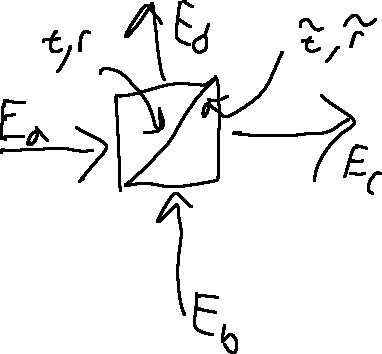
\includegraphics[width=10cm]{1-29-1.png}
	\caption*{Beamsplitter diagram}
\end{figure*}
\begin{align*}
	E_d &= rE_a + \tilde{t} E_b \\
	E_c &= tE_a + \tilde{r}E_b
\end{align*}
This is a unitary transformation so we see no loss. We can rewrite this in terms of creation/annihilation operators:
\begin{align*}
	\begin{pmatrix}
		\hat{c} \\
		\hat{d}
	\end{pmatrix} &= \begin{pmatrix}
	t & \tilde{r} \\
	r & \tilde{t}
		 \end{pmatrix}
		 \begin{pmatrix}
			 \hat{a} \\
			 \hat{b}
		 \end{pmatrix}
\end{align*}
It happens that in order to enforce unitarity we must have either:
\begin{align*}
	U &= \begin{pmatrix}
		t & r \\
		-r & t
	     \end{pmatrix} \\
	U &= \begin{pmatrix}
		t & ir \\
		ir & t
	     \end{pmatrix}
\end{align*}
We often have 50:50 beam splitters where $t=r=\frac{1}{\sqrt{2}}$ so:
\begin{align*}
	U &= \frac{1}{\sqrt{2}} \begin{pmatrix}
		1 & 1 \\
		-1 & 1
				\end{pmatrix}
\end{align*}

\subsection{Coherent states continued}
We can see that the probability to find $n$ photons is:
\begin{align*}
	P_\alpha(n) &= e^{-|\alpha|^2} \frac{(|\alpha|^2)^n}{n!} \\
	\expval{\hat{n}} &= |\alpha|^2
\end{align*}
Which is a Poisson distribution, with:
\begin{align*}
	P_\alpha(n) &= e^{-\bar{n}} \frac{\bar{n}^n}{n!}
\end{align*}
Where we also know that the standard deviation must be $\sqrt{\bar{n}}$ from the properties of the Poisson distribution.

From now on we will shift our definition of $q$ and $p$, such that:
\begin{align*}
	\hat{q} &= \frac{\hat{a} + \hat{a}^\dagger}{\sqrt{2}} \\
	\hat{p} &= \frac{\hat{a} - \hat{a}^\dagger}{i\sqrt{2}} \\
	[\hat{q},\hat{p}] &= i
\end{align*}
So then:
\begin{align*}
	\hat{a} &= \frac{\hat{q} + i\hat{p}}{\sqrt{2}} \\
	\hat{a}^\dagger &= \frac{\hat{q} - i\hat{p}}{\sqrt{2}}
\end{align*}
Therefore we can say:
\begin{align*}
	\bra{q}\ket{\alpha} &= \bra{q}\hat{D}(\alpha)\ket{0} \\
	\bra{q}\ket{\alpha} &= \bra{q}e^{\frac{\alpha - \alpha^*}{\sqrt{2}}\hat{q} - i\hat{p}\frac{\alpha + \alpha^*}{\sqrt{2}}}\ket{0} \\
	\bra{q}\ket{\alpha} &= \bra{q}e^{\frac{\alpha - \alpha^*}{\sqrt{2}}\hat{q}}e^{- i\hat{p}\frac{\alpha + \alpha^*}{\sqrt{2}}}e^\frac{-(\alpha - \alpha^*)(\alpha + \alpha^*)}{4}\ket{0} \\
	\bra{q}\ket{\alpha} &= e^\frac{-(\alpha - \alpha^*)(\alpha + \alpha^*)}{4}e^{\frac{\alpha - \alpha^*}{\sqrt{2}}q}\bra{q}e^{- i\hat{p}\frac{\alpha + \alpha^*}{\sqrt{2}}}\ket{0} \\
	\bra{q}\ket{\alpha} &= e^\frac{-(\alpha - \alpha^*)(\alpha + \alpha^*)}{4}e^{\frac{\alpha - \alpha^*}{\sqrt{2}}q}\bra{q}e^{- i\hat{p}\frac{\alpha + \alpha^*}{\sqrt{2}}}\int \frac{dp'}{2\pi}\ket{p'}\bra{p'}\ket{0} \\
	\bra{q}\ket{\alpha} &= e^\frac{-(\alpha - \alpha^*)(\alpha + \alpha^*)}{4}e^{\frac{\alpha - \alpha^*}{\sqrt{2}}q}\int \frac{dp'}{2\pi}e^{- i\hat{p'}\frac{\alpha + \alpha^*}{\sqrt{2}}}\bra{q}\ket{p'}\bra{p'}\ket{0} \\
	\bra{q}\ket{\alpha} &= e^\frac{-(\alpha - \alpha^*)(\alpha + \alpha^*)}{4}e^{\frac{\alpha - \alpha^*}{\sqrt{2}}q}\int \frac{dp'}{2\pi}e^{- i\hat{p'}\frac{\alpha + \alpha^*}{\sqrt{2}}}e^{ip'q}\psi_0(p') \\
	\bra{q}\ket{\alpha} &= e^\frac{-(\alpha - \alpha^*)(\alpha + \alpha^*)}{4}e^{\frac{\alpha - \alpha^*}{\sqrt{2}}q}\int \frac{dp'}{2\pi}e^{ip'(q-q_\alpha)}\psi_0(p') & q_\alpha &= \sqrt{2}\Re\alpha \\
	\bra{q}\ket{\alpha} &= e^\frac{-(\alpha - \alpha^*)(\alpha + \alpha^*)}{4}e^{\frac{\alpha - \alpha^*}{\sqrt{2}}q} \psi_0(q - q_\alpha)
\end{align*}
And clearly:
\begin{align*}
	\bra{q}\ket{\alpha} &= e^\frac{-(\alpha - \alpha^*)(\alpha + \alpha^*)}{4}e^{\frac{\alpha + \alpha^*}{i\sqrt{2}}p} \psi_0(p - p_\alpha) & p_\alpha &= \sqrt{2}\Im\alpha
\end{align*}
We know the overlap between two coherent states is:
\begin{align*}
	\bra{\beta}\ket{\alpha} &= e^{-\frac{|\alpha|^2 + |\beta|^2}{2} + \beta^*\alpha} \\
	|\bra{\beta}\ket{\alpha}|^2 &= e^{-|\alpha-\beta|^2}
\end{align*}
We additionally know that coherent states are overcomplete. Where we say that a complete set of states we can say:
\begin{align*}
	1 &= \sum_n \ket{n}\bra{n} \\
	1 &= \int dq \ket{q}\bra{q} \\
	1 &= \int \frac{dp}{2\pi} \ket{p}\bra{p}
\end{align*}
For coherent states we find:
\begin{align*}
	1 &- \in \frac{d^2\alpha}{\pi}\ket{\alpha}\bra{\alpha}
\end{align*}

\subsection{Wigner Representation}
We will now introduce the Wigner representation which is an example of a quasi-probability distribution.

For a classical probability distribution:
\begin{align*}
	\int \frac{dp}{2\pi} P(q,p) &= P(q) \\
	\int dq P(q,p)&= P(p) \\
	\int\int \frac{dp}{2\pi}dq P(q,p) &= 1 \\
	P(q,p) &\in \mathbb{R} \\
	P(q,p) & \geq 0
\end{align*}
We define the Wigner function:
\begin{align*}
	W_\psi(q,p) &= \frac{1}{2\pi} \int dq' \bra{q - \frac{q'}{2}}\ket{\psi}\bra{\psi}\ket{q + \frac{q'}{2}} e^{ipq'} \\
	W_\rho(q,p) &= \frac{1}{2\pi} \int dq' \bra{q - \frac{q'}{2}}\hat{\rho}\ket{q + \frac{q'}{2}} e^{ipq'} \\
	W_\rho(q,p) &= \frac{1}{2\pi} \int \frac{dp'}{2\pi} \bra{p - \frac{p'}{2}}\hat{\rho}\ket{p + \frac{p'}{2}} e^{-ipq'}
\end{align*}
Which is equivalent to the expectation value of a displaced parity operator.

We can immediately see that since this is the expectation value of the displaced parity operator, it must always have real values.
We can also see that this is normalized, and the marginals are our expected marginals.
\begin{align*}
	W(p,q) &\in \mathbb{R} \\
	\int\int \frac{dp}{2\pi}dq W(q,p) &= 1 \\
	\int \frac{dp}{2\pi} W(q,p) &= \bra{q}\hat{\rho}\ket{q} \\
	\int dq W(q,p)&= \bra{p}\hat{\rho}\ket{p}
\end{align*}
And similarly for any set of well defined orthogonal marginals. 

For the overlap of two states:
\begin{align*}
	\Tr{\hat{\rho_1}\hat{\rho_2}} &= \int\int \frac{dpdq}{2\pi} W_{\rho_1}(q,p)W_{\rho_2}(p,q)
\end{align*}
Additionally we can calculate the expectation value of an observable:
\begin{align*}
	\Tr{\hat{\rho}\hat{\Pi}} &= \int \int \frac{dqdp}{2\pi} W_\rho(q,p) W_\Pi(q,p)
\end{align*}
Additionally we can see:
\begin{align*}
	\Tr{\hat{\rho}^2} &= \int\int \frac{dqdp}{2\pi} W_\rho^2(q,p)
\end{align*}
We can use this to generate a matrix representation via:
\begin{align*}
	\rho_{mn} &=\Tr{\hat{\rho}\ket{m}\bra{n}}
\end{align*}
We can also find:
\begin{align*}
	|W(q,p)| &\leq \frac{1}{\pi}
\end{align*}

We investigate the Wigner function in practice now by considering the Wigner function of the vaccuum state:
\begin{align*}
	W_0(q,p) &=\frac{1}{2\pi} \int dq' \psi_0\left(q- \frac{q'}{2}\right)\psi_0^*\left(q + \frac{q'}{2}\right) e^{ipq'} \\
	W_0(q,p) &=\frac{1}{\pi} e^{-(q^2 + p^2)}
\end{align*}

Now turning to a coherent state, we can see that since this is really simply shifting our function in phase space, we can easily see:
\begin{align*}
	W_\alpha(q,p) &= \frac{1}{\pi} e^{-((q-q_\alpha)^2 + (p-p_\alpha)^2)} 
\end{align*}

Now looking at number states (beyond the vaccuum state):
\begin{align*}
	W_n(q,p) &=\frac{1}{2\pi} \int dq' \bra{q - \frac{q'}{2}}\ket{n}\bra{n}\ket{q + \frac{q'}{2}} e^{iq'p} \\
	W_n(q,p) &= \frac{1}{\pi}(-1)^n e^{-(q^2 + p^2)}L_n(2(q^2 + p^2))
\end{align*}
Where $L_n$ is the $n$th Laguerre polynomial:
\begin{align*}
	L_0 &= 1 \\
	l_1 &= 1-x \\
	L_2 &= \frac{1}{2}(x^2 - 4x +2)
\end{align*}
Etcetera.
So:
\begin{align*}
	W_1(q,p) &= -\frac{e^{-(q^2 + p^2)}}{\pi} (1 - 2(q^2 + p^2))
\end{align*}
Interestingly we know:
\begin{align*}
	W_1(0,0) &= -\frac{1}{\pi}
\end{align*}
We turn now to cat states which are macroscopic states entangled with microscopic systems. When we talk about this in terms of our states in quantum optics we say our cat states are states like $\ket{\alpha} + \ket{-\alpha}$. We see the Wigner function will be:
\begin{align*}
	W_\text{c.s.}(q,p) &= \frac{1}{2\pi} \int dq'\bra{q - \frac{q'}{2}}(\ket{\alpha} + \ket{-\alpha}(\bra{\alpha} + \bra{-\alpha})\ket{q + \frac{q'}{2}} 
\end{align*}
Which clearly includes a pair of terms for our individual Wigner functions for $\ket{\alpha}$ and $\ket{-\alpha}$, while we see the other two terms give us interference effects.

If we assume $\alpha$ is real, then we will see that we have a sum of coherent states in the $q$ representation, but interference effects in the $p$ state. 
Alternatively if we look at a mixture $\rho = \ket{\alpha}\bra{\alpha} + \ket{-\alpha}\bra{-\alpha}$ which doesn't see any interference effects.

We say that the negativity of the Wigner function is one way to describes how quantum a state is.

\subsection{Squeezed state}
We have two more single mode states to introduce at this point. The first of which is the thermal state, which can be well described classically. For an interesting quantum state we now turn to squeezed states.

We introduce these squeezed states with the squeezing operator:
\begin{align*}
	\hat{S}(\xi) &- e^{\frac{\xi^*\hat{a}^2 - \xi\hat{a}^\dagger\ ^2}{2}}
	\xi &= r e^{i\theta}
\end{align*}
We note that $\hat{S}$ is unitary, so $\hat{S}^\dagger \hat{S} = 1$ and $\hat{S}^\dagger(\xi) = \hat{S}(-\xi)$. We now looke at:
\begin{align*}
	\hat{S}^\dagger(\xi) \hat{a}\hat{S}(\xi)
\end{align*}
Noteing:
\begin{align*}
	\ket{\xi} &= \hat{S}(\xi)\ket{0}
\end{align*}
So we can think of this as the Heisenberg picture evolution of $\hat{a}$. For contrast with coherent states:
\begin{align*}
	\hat{D}^\dagger(\alpha)\hat{a}\hat{D}(\alpha) &=\hat{a} + \alpha \\
	\hat{D}^\dagger(\alpha)\hat{a}^\dagger\hat{D}(\alpha) &=\hat{a}^\dagger + \alpha^*
\end{align*}
Where we used:
\begin{align*}
	e^{\hat{A}} \hat{B} e^{-\hat{A}} &= \hat{B} +  [\hat{A},\hat{B}] + \frac{1}{2} [\hat{A},[\hat{A},\hat{B}]] + \ldots \\
\end{align*}
For the squeezing operator we see:
\begin{align*}
	\hat{S}^\dagger(\xi)\hat{a}\hat{S}(\xi) &= \hat{a}\cosh(r)  - \hat{a}^\dagger e^{i\theta} \sinh(r) \\
	\hat{S}^\dagger(\xi)\hat{a}^\dagger\hat{S}(\xi) &= \hat{a}^\dagger\cosh(r)  - \hat{a} e^{-i\theta} \sinh(r)
\end{align*}
And clearly:
\begin{align*}
	\hat{S}^\dagger \hat{q}\hat{S} &= \frac{1}{\sqrt{2}}\left( (\hat{a} + \hat{a}^\dagger) \cosh(r) - (\hat{a} e^{-i\theta} + \hat{a}^\dagger e^{i\theta})\sinh(r)\right) \\
	\hat{S}^\dagger \hat{p}\hat{S} &= \frac{1}{\sqrt{2}i}\left( (\hat{a} - \hat{a}^\dagger) \cosh(r) + (\hat{a} e^{-i\theta} - \hat{a}^\dagger e^{i\theta})\sinh(r)\right)
\end{align*}
If we choose $\theta = 0$ then we have:
\begin{align*}
	\hat{S}^\dagger \hat{q}\hat{S} &= \hat{q}(\cosh(r) - \sinh(r)) \\
	\hat{S}^\dagger \hat{q}\hat{S} &= \hat{q}e^{-r} \\
	\hat{S}^\dagger \hat{p}\hat{S} &= \hat{p}(\cosh(r) + \sinh(r)) \\
	\hat{S}^\dagger \hat{p}\hat{S} &= \hat{p}e^r
\end{align*}
Therefore when we look at our squeezed states:
\begin{align*}
	W_\xi(q,p) &= \frac{1}{2\pi}\int dq' \bra{q-\frac{q'}{2}}\ket{\xi}\bra{\xi}\ket{q + \frac{q'}{2}} e^{ipq'}
\end{align*}
Since:
\begin{align*}
	\bra{q}\ket{\psi} &= \bra{q}\hat{S}\ket{0} \\
	\bra{q}\ket{\psi} &= \bra{q}\hat{S}\int dq'\ket{q'}\bra{q'}\ket{0} \\
	\hat{q}\hat{S}\ket{q} &= e^{-r} q\hat{S}\ket{q}
\end{align*}
Which means that this is still an eigenstate of $\hat{q}$ but with eigenvalue $qe^{-r}$, so:
\begin{align*}
	\bra{q}\ket{\psi} &= \bra{q e^{-r}}\ket{0} \\
	W_\xi(q,p) &= \frac{1}{2\pi}\int dq' \bra{(q-\frac{q'}{2})e^{-r}}\ket{0}\bra{0}\ket{e^{r}(q + \frac{q'}{2})} e^{ipq'}
\end{align*}
So we can see that this will be the vaccuum state with $q\to qe^{-r}$, and $p\to pe^{r}$. So our Wigner function becomes:
\begin{align*}
	W_\xi(q,p) &= W_0(qe^{r},pe^{-r})
\end{align*}
We now look at the variances of the quadratures:
\begin{align*}
	\Delta q^2 &= \bra{\xi}\hat{q}^2\ket{\xi} - \bra{\xi}\hat{q}\ket{\xi}^2 \\
	\Delta q^2 &= \bra{0}e^{-2r}\hat{q}2\ket{0} - \bra{0}e^{-r}\ket{0}^2 \\
	\Delta q^2 &= e^{-2r}(\bra{0}\hat{q}2\ket{0} - \bra{0}\ket{0}^2) \\
	\Delta q^2 &= e^{-2r}\Delta_0 q^2 \\
	\Delta p^2 &= e^{2r}\Delta_0 p^2
\end{align*}

\subsection{Coherent state representation}
We now introduce another representation of our states. We want to use coherent states to represent our state, this is sometimes call the Glauber-Sadershan, or P-function representation.

We consider a density operator $\hat{\rho}$:
\begin{align*}
	\hat{\rho} &= \int d^2\alpha P(\alpha,\alpha^*)\ket{\alpha}\bra{\alpha}
\end{align*}
Where we can say:
\begin{align*}
	p_\alpha &= \frac{\alpha - \alpha^*}{\sqrt{2}i} &
	q_\alpha &= \frac{\alpha + \alpha^*}{\sqrt{2}}
\end{align*}
Our representation is initially quite strange as it appears to be a diagonal representation of our state, but since the coherent states are non-orthogonal we can see that isn't exactly the case:
\begin{align*}
	\bra{-\beta}\hat{\rho}\ket{\beta} &= \int d^2\alpha P(\alpha,\alpha^*) \bra{-\beta}\ket{\alpha}\bra{\alpha}\ket{\beta} \\
	P(\alpha,\alpha^*) &= \frac{e^{|\alpha|^2}}{2\pi}\int \bra{-\beta}\hat{\rho}\ket{\beta} e^{|\beta|^2} e^{-\beta\alpha^* + \beta^*\alpha} d^2\beta
\end{align*}
Therefore:
\begin{align*}
	P_{\alpha_0}(\alpha,\alpha^*) &= \frac{e^{|\alpha|^2}}{2\pi} \int d^2\beta \bra{-\beta}\ket{\alpha_0}\bra{\alpha_0}\ket{\beta} e^{|\beta|^2} e^{-\beta\alpha^*} e^{\beta^*\alpha} \\
	P_{\alpha_0}(\alpha,\alpha^*) &= \frac{e^{|\alpha|^2}}{2\pi} \int d^2\beta e^{-\beta(\alpha^*-\alpha_0^*)} e^{\beta^*(\alpha-\alpha_0)} \\
	P_{\alpha_0}(\alpha,\alpha^*) &= \delta(\alpha - \alpha_0)
\end{align*}
We can see that for a Fock state:
\begin{align*}
	P_n(\alpha,\alpha^*) &= \frac{e^{|\alpha|^2}}{n!} \frac{\partial^n}{\partial \alpha^n}\frac{\partial^n}{\partial\alpha^*\ ^n} \delta(\alpha)
\end{align*}
Which is something that clearly cannot be measured. In order to suppliment this representation we additionally include the (Husini) Q-function representation:
\begin{align*}
	Q_\rho(\alpha,\alpha^*) &= \frac{\bra{\alpha}\hat{\rho}\ket{\alpha}}{2\pi}
\end{align*}
Clearly we can see:
\begin{align*}
	Q_{\alpha_0}(\alpha,\alpha^*) &= \frac{|\bra{\alpha}\ket{\alpha_0}|^2}{2\pi}
\end{align*}
We can then see:
\begin{align*}
	Q_\rho(\alpha,\alpha^*) &= \frac{1}{2\pi} \int d^2\alpha' W_\rho(\alpha', \alpha'\ ^*) e^{-(\alpha - \alpha')^2} e^{-(\alpha^* - \alpha'\ ^*)^2} \\
	W_\rho(\alpha,\alpha^*) &= \frac{1}{2\pi} \in d^2\alpha' P(\alpha',\alpha'\ ^*) e^{-(\alpha-\alpha')^2} e^{-(\alpha^* - \alpha'\ ^*)^2}
\end{align*}
Which allows us to compute:
\begin{align*}
	\Tr{\hat{\rho}\hat{\sigma}} &= \int d^2\alpha P_\rho(\alpha)Q_\sigma(\alpha)
\end{align*}
Where we can charactorize a detector by inputting coherent states and calculating $Q$, and try to determine the input state via reversing this integral.

\section{Interference/Coherence}
When we think of interference we think of things like the double slit, and michelson-morley experements.

In order to probe coherence we consider young's experement, where we filter to two points from a single light source. For something like the sun we have two sources that aren't physically connected.
In this experiment we will measure the intensity of light averaged over time. Expressed mathematically we measure:
\begin{align*}
	\int_{t-\frac{T}{2}}^{t+\frac{T}{2}} |E(t')|^2 dt'
\end{align*}
Where our detecter bandwidth is $\frac{1}{T}$. This could be changed to be related to some windowing function instead, where this detector is the detector generated by a tophat function.
If we have two different $E$ fields from our source we can say our irradiance is:
\begin{align*}
	I &= \int_{t-\frac{T}{2}}^{t+\frac{T}{2}} |E(t')|^2 dt' \\
	I &= \int_{t-\frac{T}{2}}^{t+\frac{T}{2}} |E_1(t') + E_2(t')|^2 dt' \\
	I &= I_1(t) + I_2(t) + 2\Re{\int dt E_1^* E_2} \\
	\int dt' E_1^* E_2 &= \int dt' |E_1| e^{-i\phi_1} |E_2| e^{i\phi_2} \\
	\int dt' E_1^* E_2 &= \int dt' |E_1| |E_2| e^{i\Delta \phi_{12}}
\end{align*}
Which if $\phi_1$ and $\phi_2$ are uncorrelated, then we should have no interference term. We think of light from the sun as random so we expect there to be no interference term, or in other words no coherence.

In this context when we talk about coherence we mean fixed phase relationships between two different fields.

\begin{figure*}[h]
	\centering
	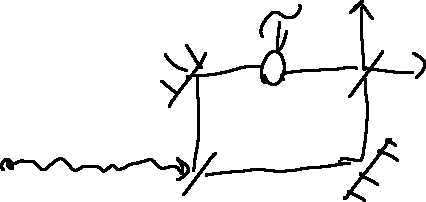
\includegraphics[width=6cm]{2-10-1.png}
	\caption*{Mach-Zender}
\end{figure*}
Now we consider splitting our point source at a beam splitter and then recombining it in a ``Mach-Zender'' interferometer, which we see will give us:
\begin{align*}
	E_\text{up} &= -rr'E_1(t+\tau) + tt' E_1(t) \\
	E_\text{r} &= tr' E_1(t) + rt' E_1(t+\tau)
\end{align*}
If we now choose 50/50 beam splitters so $r=t=\frac{1}{\sqrt{2}}$:
\begin{align*}
	E_\text{up} &= \frac{1}{2}(E_1(t) - E_1(t+\tau)) \\
	E_\text{r} &= \frac{1}{2} (E_1(t) + E_1(t+\tau))
\end{align*}
S o our irradiance in this situation becomes:
\begin{align*}
	I_r(t,\tau) &= \frac{1}{4} \int dt' \left[|E_1(t')|^2 + |E_1(t' + \tau)|^2 + 2\Re{|E_1(t')||E_1(t' + \tau)| e^{i(\phi_1(t') - \phi_1(t'+\tau))}}\right]
\end{align*}
In order to analyze this we now look at this in the fourier domain (we vary $\tau$ and then do a fourier transform in an experiment) here we will remove the terms that don't correspond to the coherences, 
potentially by simply measuring them and canceling them, or by ignoring the low frequency components:
\begin{align*}
	\tilde{I}_r(t,\omega) &= \int e^{i\omega\tau} I_r(t,\tau) d\tau \\
	\tilde{I}_r(t,\omega) &= \frac{1}{4}\int d\tau e^{i\omega\tau} \int dt'(2|E_1(t')||E_1(t'+ \tau)|\cos \Delta\phi_{12}(t';\tau) + \omega_0\tau
\end{align*}
Where $\omega_0$ is the wave's ``carrier'' frequency.
\begin{align*}
	\tilde{E}(\omega) &= A(\omega-\omega_0) & A(\omega) &= \mathcal{F}(|E_(t)|) \\
	\tilde{I}_r(t,\omega) &= \frac{1}{2}\int d\tau e^{i\omega\tau} \int dt'\Re(E_1^*(t')E_1(t'+ \tau)) \\
	\tilde{I}_r(t,\omega) &= \frac{1}{2}\int d\tau e^{i\omega\tau} \int dt'\Re\left(\int \frac{d\omega'}{2\pi} e^{i\omega't'} \tilde{E}(\omega')\int \frac{d\bar{\omega}}{2\pi} e^{-i\bar{\omega}(t'+\tau)} \tilde{E}^*(\bar{\omega})\right) \\
	\tilde{I}_r(t,\omega) &= \frac{1}{2}\Re\left(\int \frac{d\omega'}{2\pi}\int \frac{d\bar{\omega}}{2\pi} \int dt'e^{i(\omega' - \bar{\omega})} \tilde{E}(\omega')  \tilde{E}^*(\bar{\omega})\int d\tau  e^{i\tau(\omega-\bar{\omega})}\right) \\
	\tilde{I}_r(t,\omega) &= \frac{1}{2}\Re\left(\int d\omega'\int d\bar{\omega} \delta(\omega' - \bar{\omega}) \tilde{E}(\omega')  \tilde{E}^*(\bar{\omega})\delta(\omega-\bar{\omega})\right) \\
	\tilde{I}_r(t,\omega) &= \frac{1}{2}\Re\left(\tilde{E}(\omega)  \tilde{E}(\omega)\right) \\
	\tilde{I}_r(t,\omega) &= \frac{1}{2}|\tilde{E}(\omega)|^2
\end{align*}
Which gives us a spectral intensity of our light. This relation is the ``Weiner-Khinchin'' theorem. We call $\expval{E^*(t)E(t+\tau)}$ the first order correlation function. The Weiner-Khinchin theorem explicitly says:
\begin{align*}
	\expval{|\tilde{E}(\omega(|^2} &= \mathcal{F}(\expval{E^*(t)E(t+\tau)})
\end{align*}
We add quantum to this picture by replacing our field amplitudes here into operators
\subsection{Degree of first order coherence}
\begin{align*}
	g_{ij}^{(1)} (\tau,r) &= \frac{\expval{\hat{E}_i^{(-)}(x,t)\hat{E}_j^{(+)}(x+ r,t+\tau)}}{\sqrt{I_i(x,t) I_j(x+r,t+\tau)}}
\end{align*}
Describes our coherences, where $i,j$ label our polarizations/modes and this is an implicit function of $x,t$. Looking at fixed positions we can see this becomes:
\begin{align*}
	g^{(1)}(t,\tau) &= \frac{\expval{\hat{E}_i^{(-)}(t)\hat{E}_j^{(+)}(t+\tau)}}{\sqrt{I_i(t) I_j(t+\tau)}}
\end{align*}
If we have a stationary distribution, or if we have a detector that averages over the entire pulse length, then we have:
\begin{align*}
	g^{(1)}(\tau) &= \frac{\expval{\hat{E}_i^{(-)}(0)\hat{E}_j^{(+)}(\tau)}}{\sqrt{I_i(0) I_j(\tau)}}
\end{align*}
Which we write as:
\begin{align*}
	g^{(1)}(\tau) &= \frac{\expval{\hat{a}^\dagger(t)\hat{a}(t+\tau)}}{\sqrt{\expval{\hat{a}^\dagger(t)\hat{a}}\expval{\hat{a}^\dagger(t+\tau)\hat{a}(t+\tau)}}}
\end{align*}
Which will tell us about the spectrum of our source. On the other hand $g^{(1)}(x,t,r,\tau)$ tells about the modes of the source. This will not tell about the state of the field. To illustrate this we consider a single photon and a coherent state occupying the same mode:
\begin{align*}
	\hat{a}(t)\ket{1}_\psi &= \int dt' \hat{a}\hat{a}^\dagger \phi(t') \vac \\
	\hat{a}(t)\ket{1}_\psi &= \int dt' \delta(t-t') \phi(t') \vac \\
	\hat{a}(t)\ket{1}_\psi &= \phi(t) \vac
\end{align*}
So we can say:
\begin{align*}
	\expval{\hat{a}^\dagger(t) \hat{a}(t+\tau)} &= \psi^*(t)\psi(t+\tau) \\
	g^{(1)}(\tau) &= \frac{\psi^*(t)\psi(t+\tau)}{\sqrt{|\psi(t)|^2|\psi(t+\tau)|^2}}
\end{align*}
We repeat this for the coherent state:
\begin{align*}
	\expval{\hat{a}^\dagger(t)\hat{a}(t+\tau)} &= \psi^*(t)\psi(t+\tau)|\alpha|^2 \\
	g^{(1)}(\tau) &= \frac{\psi^*(t)\psi(t+\tau)|\alpha|^2}{|\alpha|^2\sqrt{|\psi(t)|^2|\psi(t+\tau)|^2}}\\
	g^{(1)}(\tau) &= \frac{\psi^*(t)\psi(t+\tau)}{\sqrt{|\psi(t)|^2|\psi(t+\tau)|^2}}
\end{align*}
\subsection{Degree of 2nd order coherence}
So far we have only extracted information about the modes that we are occupying. The first order coherence can be thought of as containing information about amplitude correlations.
We will now look at the intensity correlations, which will tell us about the states in the modes.
These are related to Hanbury-Brown and Twiss experiment, which let us measure the diameters of stars without using interferometers.

We define:
\begin{align*}
	g^{(2)}(\tau) &= \frac{\expval{\hat{a}^\dagger(t)\hat{a}^\dagger(t+\tau)\hat{a}(t+\tau)\hat{a}(t)}}{\expval{\hat{a}^\dagger(t)\hat{a}}\expval{\hat{a}^\dagger(t+\tau)\hat{a}(t+\tau)}}
\end{align*}
We measure this using something like a Hanbury-Brown Twiss setup.
\begin{figure*}[h]
	\centering
	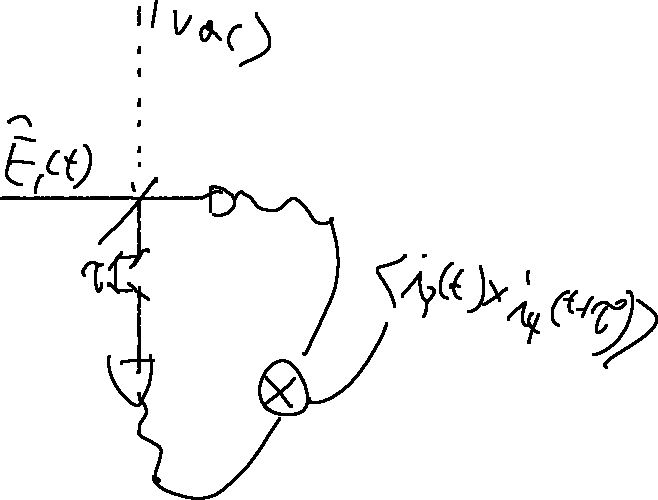
\includegraphics[width=6cm]{2-10-2.png}
	\caption*{Hanbury-Brown Twiss}
\end{figure*}

Our measurement will be:
\begin{align*}
	\expval{\hat{I}_3(t) \hat{I}_4(t+\tau)}
\end{align*}
If we input a single photon state we find after the beam splitter our state is:
\begin{align*}
	\ket{\psi} &= \frac{1}{\sqrt{2}}(\ket{1}_3\ket{0}_4 + \ket{0}_3\ket{1}_4)
\end{align*}
So then:
\begin{align*}
	\expval{\hat{a}_3^\dagger(t)\hat{a}^\dagger_4(t+\tau)\hat{a}_4(t+\tau)\hat{a}(t)} &= 0
\end{align*}
In contrast a coherent state gives us:
\begin{align*}
	\expval{\hat{a}_3^\dagger(t)\hat{a}^\dagger_4(t+\tau)\hat{a}_4(t+\tau)\hat{a}(t)} &= \frac{1}{4} \expval{(\hat{a}_1^\dagger(t) - \hat{a}_2^\dagger(t))(\hat{a}^\dagger_1(t+\tau) +\hat{a}^\dagger_2(t+\tau) +\ldots}
\end{align*}
If we drop all $\hat{a}_2$ terms since we have assumed that our starting state for the 2 modes is $\vac$, so we have:
\begin{align*}
	\expval{\hat{a}_3^\dagger(t)\hat{a}^\dagger_4(t+\tau)\hat{a}_4(t+\tau)\hat{a}(t)} &= \frac{1}{4} \expval{\hat{a}_1^\dagger(t)\hat{a}^\dagger_1(t+\tau)\hat{a}_1(t+\tau)\hat{a}_1(t)}
\end{align*}
If we input a coherent state we find:
\begin{align*}
	\expval{\hat{a}_3^\dagger(t)\hat{a}^\dagger_4(t+\tau)\hat{a}_4(t+\tau)\hat{a}(t)} &= \frac{1}{4} |\alpha|^4 |\psi(t)|^2|\psi(t+\tau)|^2
\end{align*}
And dividing by the normalizations we see:
\begin{align*}
	g^{(2)}(\tau) &= \frac{|\alpha|^4 |\psi(t)|^2|\psi(t+\tau)|^2}{|\alpha|^4 |\psi(t)|^2|\psi(t+\tau)|^2} \\
	g^{(2)}(\tau) &= 1
\end{align*}
We note:
\begin{align*}
	g^{(2)} &= 0 & \text{single} \\
	g^{(2)} &= 1 & \text{coherent} \\
	g^{(2)} &= 2 & \text{thermal} \\
	g^{(2)} &\geq 2 & \text{squeezed}
\end{align*}

We define a function for the coincidence counts:
\begin{align*}
	G^{(2)} &= \expval{\hat{a}^\dagger(t) \hat{a}^\dagger(t+\tau) \hat{a}(t+\tau)\hat{a}(t)}
\end{align*}
And for a two photon state:
\begin{align*}
	G^{(2)} &= \bra{2}_\psi\hat{a}^\dagger(t) \hat{a}^\dagger(t+\tau) \hat{a}(t+\tau)\hat{a}(t)\ket{2}_\psi \\
	G^{(2)} &= \bra{2}_\psi\hat{a}^\dagger(t) \hat{a}^\dagger(t+\tau) \hat{a}(t+\tau)\hat{a}(t)\frac{(\hat{a}^\dagger)^2}{\sqrt{2}}\vac \\
	G^{(2)} &= \bra{2}_\psi\hat{a}^\dagger(t) \hat{a}^\dagger(t+\tau) \hat{a}(t+\tau)\frac{2\psi(t)(\hat{a}^\dagger)}{\sqrt{2}}\vac \\
	G^{(2)} &= \bra{2}_\psi\hat{a}^\dagger(t) \hat{a}^\dagger(t+\tau) \frac{2\psi(t)\psi(t+\tau)}{\sqrt{2}}\vac \\
	G^{(2)} &= \frac{4|\psi(t)|^2|\psi(t+\tau)|^2}{2} \\
	G^{(2)} &= 2|\psi(t)|^2|\psi(t+\tau)|^2
\end{align*}
From which we can clearly see:
\begin{align*}
	g^{(2)} &= \frac{1}{2}
\end{align*}
If we look at a photon emitter, at the time of emission:
\begin{align*}
	g^{2}(0) &= \frac{\expval{\hat{a}^\dagger\ ^2\hat{a}^2}}{\expval{\hat{a}^\dagger\hat{a}}^2}
\end{align*}
Where the denometer is clearly:
\begin{align*}
	\expval{\hat{a}^\dagger\hat{a}}^2 &= \expval{\hat{n}}^2
\end{align*}
And the numerator is:
\begin{align*}
	\expval{\hat{a}^\dagger\ ^2\hat{a}^2} &= \expval{\hat{n}^2} - \expval{\hat{n}} 
\end{align*}
So then:
\begin{align*}
	g^{(2)}(0) &= \frac{\expval{\hat{n}^2} - \expval{\hat{n}}}{\expval{\hat{n}}^2} \\
	g^{(2)}(0) &= \frac{\Delta n^2 + \expval{\hat{n}}^2 - \expval{\hat{n}}}{\expval{\hat{n}}^2} \\
	g^{(2)}(0) &= 1 + \frac{\Delta n^2  - \expval{\hat{n}}}{\expval{\hat{n}}^2} \\
	g^{(2)}(0) &= 1 +   - \frac{1}{\bar{n}} + \frac{\Delta n^2}{\bar{n}^2}
\end{align*}
Which clearly gives us one for the Poissonian photon number statistics associated with the coherent state.
If we have sub Poisson statistics we say $g^{(2)} < 1$, we typically call this non-classical light. 
Fock states will have sub-Poisson statistics, and since $\Delta n^2 = 0$ for these states we clearly find $g^{(2)}(0) = 1 - \frac{1}{n}$.
As we populate more and more photons into our state we find that this approaches 1 and we have trouble distinguishing it from the coherent state.
For the squeezed state we find $g^{(2)}(0) = 3 + \frac{1}{\expval{n}}$.
\subsection{Mixed states}
We say that states with some classical uncertainty can be represented by density operators. The example we look at is the ``thermal'' state of light. This can model all sorts of natural sources, like the sun, fire, or even human body heat.
The density operator representation of a thermal state is given by something of the form:
\begin{align*}
	\hat{\rho} &= \sum_n p_n \ket{n}\bra{n}
\end{align*}
When we say that this has no coherences that refers to the fact that we don't have any off-diagonal elements of the density matrix, i.e:
\begin{align*}
	\rho_{nm} &= a_n \delta_{nm}
\end{align*}
For a coherent state we do have these coherences, in fact:
\begin{align*}
	\rho_{nm} &= e^{-|\alpha|^2} \frac{\alpha^n\alpha^*\ ^m}{\sqrt{n!m!}}
\end{align*}
For the thermal state we know:
\begin{align*}
	p_n &= \frac{e^{-\frac{n\hbar\omega}{k_B T}}}{1- e^{-\frac{\hbar\omega}{k_B T}}}
\end{align*}
Which can be written as:
\begin{align*}
	p_n &= \frac{\bar{n}^n}{(1+\bar{n})^{n+1}}
\end{align*}
\subsection{Hong-Oh-Mandel interference}
Hong-Oh-Mandel interference (also known as two photon interference) is a non-classical intereference effect.
\begin{figure*}[h]
	\centering
	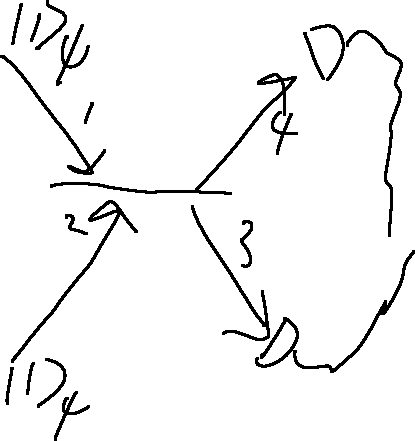
\includegraphics[width=6cm]{2-12-1.png}
	\caption*{Hong-Oh-Mandel}
\end{figure*}
We can see that probability of getting a  coincidence here is:
\begin{align*}
	P &\propto \expval{\hat{a}^\dagger_3\hat{a}_3\hat{a}^\dagger_4\hat{a}_4}
\end{align*}
We can look at this probability by propogating our states, starting with:
\begin{align*}
	\ket{\psi}_\text{in} &= \hat{a}^\dagger_{\psi1}\hat{a}^\dagger_{\psi2}\vac
\end{align*}
And we find that the output is then:
\begin{align*}
	\ket{\psi}_\text{out} &= \frac{1}{2} \left(\hat{a}_{\psi3}^\dagger + \hat{a}_{\psi4}^\dagger\right)\left(\hat{a}_{\psi3}^\dagger - \hat{a}_{\psi4}^\dagger\right)\vac \\
	\ket{\psi}_\text{out} &= \frac{\sqrt{2}}{2} \left(\ket{2}_{\psi3} + \ket{2}_{\psi4}\right)
\end{align*}
Which shockingly gives us either 2 photons at one detector, or two photons at the other, and never a coincidence!
In hindsight this is what we should expect, as bosons tend to clump together. In contrast if we fired two fermions into a beamsplitter like this we would expect to find the electrons never arriving at the same port.

\begin{figure*}[h]
	\centering
	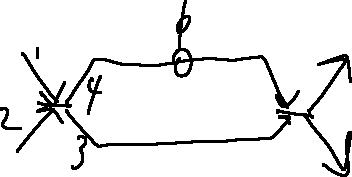
\includegraphics[width=6cm]{2-12-2.png}
	\caption*{NOON interferemoter}
\end{figure*}
Repeating this experement with an additional interference, and a phase we find our coincidence count is:
\begin{align*}
	P &\propto \frac{1-\cos2\phi}{2}
\end{align*}
Which gives us a more sensative measurement of our phase! This is because at the first beamsplitter we have prepared a NooN state.

In order to test Hong-Oh-Mandel interference in the lab, they added a time delay to one arm of their interferometer
\begin{figure*}[h]
	\centering
	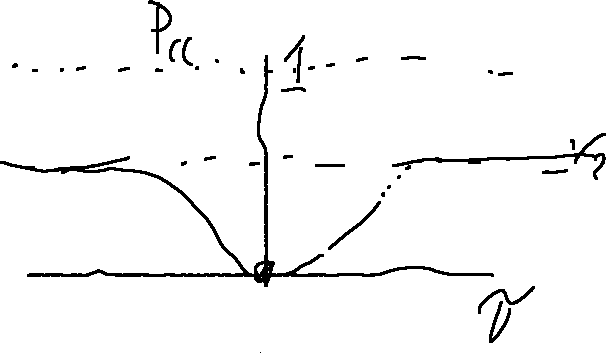
\includegraphics[width=6cm]{2-17-1.png}
	\caption*{Hong "dip"}
\end{figure*}
It can quickly be shown that the coincidence amplitude with our delay is:
\begin{align*}
	\ket{cc} &= \frac{1}{2}(\hat{a}_{4\psi}^\dagger\hat{a}_{3\phi}^\dagger -\hat{a}_{3\psi}^\dagger\hat{a}_{4\phi}^\dagger)\vac \\
	P_{cc} &= \frac{1}{4} \bra{\text{vac}}(\hat{a}_{3\phi}\hat{a}_{4\psi} -\hat{a}_{4\phi}\hat{a}_{3\psi})(\hat{a}_{4\psi}^\dagger\hat{a}_{3\phi}^\dagger -\hat{a}_{3\psi}^\dagger\hat{a}_{4\phi}^\dagger)\vac \\
	P_{cc} &= \frac{1}{4} (2 - \bra{\text{vac}}(\hat{a}_{3\phi}\hat{a}_{4\psi}\hat{a}_{3\psi}^\dagger\hat{a}_{4\phi}^\dagger - \hat{a}_{3\psi}\hat{a}_{3\phi}^\dagger\hat{a}_{4\phi}\hat{a}_{4\psi}^\dagger)\vac)
\end{align*}
We know $[\hat{a}_\psi,\hat{a}_\phi^\dagger] = (\psi|\phi) = \int \frac{d\omega}{2\pi} \tilde{\psi}^*(\omega)\tilde{\phi}(\omega)$, Therefore ($\hat{a}_{3\phi}\hat{a}_{3\psi}^\dagger = \hat{a}_{3\psi}^\dagger\hat{a}_{3\phi} + (\psi|\phi)$:
\begin{align*}
	P_{cc} &= \frac{1}{4} (2 - 2\Re{\bra{\text{vac}} [\hat{a}_{3\psi}^\dagger\hat{a}_{3\phi} + (\psi|\phi)][\hat{a}_{4\phi}^\dagger\hat{a}_{4\psi} + (\phi|\psi)]}) \\
	P_{cc} &= \frac{1}{4} (2 - 2|(\phi|\psi)|^2)
\end{align*}
If we assume we have a gaussian temporal mode, then we expect this term to go as $e^{-\frac{\tau^2}{T^2}}$, which is exactly what was observed in Hong Oh and Mandel's experiment. Clearly we would expect our two photon rates to be the compliment of the 1 photon rates.

We now turn our attention to visibility in interference effects. We define the visibility of an interferometer as $\frac{I_\text{max} - I_\text{min}}{I_\text{max} + I_\text{min}}$.
For a classical Michaelson interferometer, we predict a unit visibility, but many practical effects limit this, such as mismatched losses in the arms. This gives us a visibility of $\frac{2\tau}{1+\tau^2}$.
In the quantum sense this can be though of as introducing distinguishability between the two paths. This can additionally be introduced by changing the mode of light as it passes through one of the paths.
In our Hong mandel interference we can talk about our visibility as $\frac{P_{cc}(\infty) - P_{cc}(0)}{P_{cc}(\infty)}$. For Hong-Oh-Mandel this is $|(\phi|\psi)|^2$.

We can talk about single photons in terms of single photon density operators:
\begin{align*}
	\hat{\rho} &= \sum_m \ket{1}_{\psi m}\bra{1}_{\psi m} p_m
\end{align*}
Which when this is the input to both sides of the interferometer will give us a visibility of $1-\Tr{\hat{\rho}^2}$.
Post selection using measurement on only one port gives us a non-linear interaction. This is the basis of linear-optics quantum computing.

\subsection{Two mode squeezed vacuum}
We introduce our new squeezing operator:
\begin{align*}
	\hat{S}_{12}(\xi) &= e^{\xi^* \hat{a}_1\hat{a}_2 - \xi\hat{a}_1^\dagger\hat{a}_2^\dagger}
\end{align*}
Where these two modes are fully orthogonal. Our two mode squeezed vaccuum state is:
\begin{align*}
	\ket{\text{TMSV}_\xi}_{12} &= \hat{S}_{12} (\xi)\vac
\end{align*}
We now look at this state in term of different representations of it. Clearly we know that our two modes must always have the same number of photons.

We first look at our quadratures:
\begin{align*}
	\hat{q}_\pm &= \frac{\hat{q}_1 \pm \hat{q}_2}{2} \\
	\hat{p}_\pm &= \frac{\hat{p}_1 \pm \hat{p}_2}{2}
\end{align*}
And we can see that our commutators are simply:
\begin{align*}
	[\hat{q}_+,\hat{p}_+] &= \frac{i}{2} \\
	[\hat{q}_-,\hat{p}_-] &= \frac{i}{2} \\
	[\hat{q}_+,\hat{p}_-] &= 0 \\
	[\hat{q}_-,\hat{p}_+] &= 0
\end{align*}
We say:
\begin{align*}
	\hat{S}_{12}^\dagger(\xi)\hat{a}_1\hat{S}_{12}(\xi) &= \hat{a}_1\cosh r - e^{i\theta} \hat{a}_2^\dagger\sinh r \\
	\hat{S}_{12}^\dagger(\xi)\hat{a}_2\hat{S}_{12}(\xi) &= \hat{a}_2\cosh r - e^{i\theta}\hat{a}_1^\dagger \sinh r
\end{align*}
So:
\begin{align*}
	\expval{\hat{q}_+} &= \bra{\text{vac}}\hat{S}_{12}^\dagger(\xi)\hat{q}_+\hat{S}_{12}(\xi)\vac \\
	\expval{\hat{q}_+} &= 0
\end{align*}
But:
\begin{align*}
	\expval{\hat{q}_+^2} &= \bra{\text{vac}}\hat{S}_{12}^\dagger(\xi)\hat{q}_+\hat{S}_{12}(\xi)\hat{S}^\dagger_{12}(\xi)\hat{q}_+\hat{S}_{12}(\xi)\vac
\end{align*}
Where we can show (for a certain choice of $\theta$):
\begin{align*}
	\hat{S}^\dagger\hat{q}_+\hat{S} &= q_1\cosh r - q_2\sinh r
\end{align*}
So then:
\begin{align*}
	\expval{\hat{q}_+^2} &= \frac{1}{4} e^{-2r} \\
	\expval{\hat{p}_+^2} &= \frac{1}{4} e^{2r}
\end{align*}
We can now look at these operators in order to find our number representation, which is:
\begin{align*}
	\ket{\xi}_{12} &= \frac{1}{\cosh r} \sum_n (-1)^n e^{in\theta}(\tanh r)^n \ket{n}_1\ket{n}_2
\end{align*}
This can be thought of the result of a two mode spontaneous parametric down conversion (SPDC).

Clearly:
\begin{align*}
	\expval{\hat{n}_1 - \hat{n}_2} &= 0 \\
	\expval{\hat{n}_1} &= \sinh^2 r
\end{align*}
We can also see:
\begin{align*}
	\hat{\rho}_1 &=\Tr_2\{\ket{\xi}_{12}\bra{\xi}_{12}\} \\
	\hat{\rho}_1 &=\sum_m |\lambda|^{2n}\ket{m}_1\bra{m}_1
\end{align*}
Which has thermal statistics!

We can tell that these systems will arrise from things with Hamiltonians of the form $\hat{H} = \hat{a}_1\hat{a}_2 + \hercon$

We can say:
\begin{align*}
	\hat{S}^\dagger \hat{q}_\pm \hat{S} &= e^{\mp r} \hat{q}_\pm \\
	\hat{S}^\dagger \hat{p}_\pm \hat{S} &= e^{\pm r} \hat{p}_\pm \\
\end{align*}

Looking now at the Wigner representation:
\begin{align*}
	W_{12}(q_1,p_1;q_2,p_2) &= \frac{1}{4\pi^2} \int dq'\int dq'' \bra{q_1 - \frac{q'}{2}}\bra{q_2 - \frac{q''}{2}} \ket{\xi}_{12}\bra{\xi}_{12}\ket{q_1 + \frac{q'}{2}}\ket{q_2 + \frac{q''}{2}} e^{ip_1q'} e^{ip_2q''}
\end{align*}
In order to evaluate this we want to look at the $q_\pm$ basis:
\begin{align*}
	\bra{q_+}\bra{q_-}\ket{\xi} &= \psi_0(q_+ e^{-r})\psi_0(q_- e^r)
\end{align*}
Looking at the quadratures in terms of creation and annihilation operators:
\begin{align*}
	\hat{q}_\pm &= \frac{\hat{a}_1 \pm \hat{a}_2}{2} + \frac{\hat{a}_1^\dagger \pm \hat{a}_2^\dagger}{2}
\end{align*}
We can recognize that this is the same as a 50:50 beamsplitter transformation. We can also observe that the squeezed state seems to be simply the two seperate squeezed states (with perpendicular squeezing) combined at a beamsplitter.
Interestingly, the two seperate states that we have combined are not entangled, but the combined state is entangled. From this we can see that entanglement is a product of the mode basis that we are looking at the system with.

We can use our beamsplitter here to determine the Wigner function by looking at this as a change of basis for our Wigner function:
\begin{align*}
	q_1 &= \frac{q_+ + q_-}{\sqrt{2}} \\
	q_2 &= \frac{q_+ - q_-}{\sqrt{2}} \\
	p_1 &= \frac{p_+ + p_-}{\sqrt{2}} \\
	p_2 &= \frac{p_+ - p_-}{\sqrt{2}}
\end{align*}
So then:
\begin{align*}
	\bra{q_1}\bra{q_2}\ket{\xi} &= \psi_0(\frac{q_1 + q_2}{\sqrt{2}} e^{-r})\psi_0(\frac{q_1 - q_2}{\sqrt{2}} e^r)
\end{align*}

\subsection{Beamsplitter transoformations}
We now look at how our Wigner function transforms with a pair of general two mode states in a beamsplitter. We first note that a beamsplitter transformation is equivalent to a mode basis change.
After a 50:50 beamsplitter we transform our creation and annihilation operators:
\begin{align*}
	\hat{a}_1 &l\to \frac{1}{\sqrt{2}} (\hat{a}_3 -\hat{a}_4) \\
	\hat{a}_1 &l\to \frac{1}{\sqrt{2}} (\hat{a}_3 -\hat{a}_4) \\
	\hat{a}_3 &= \frac{1}{\sqrt{2}} (\hat{a}_1 +\hat{a}_2) \\
	\hat{a}_4 &= -\frac{1}{\sqrt{2}} (\hat{a}_1 -\hat{a}_2) \\
\end{align*}
And similarly the quadratures transfom as:
\begin{align*}
	\hat{q}_3 &= \frac{\hat{q}_1 + \hat{q}_2}{\sqrt{2}}
	\hat{q}_4 &= \frac{\hat{q}_1 - \hat{q}_2}{\sqrt{2}}
\end{align*}
And our Wigner functions become:
\begin{align*}
	W_{12}(q_1,p_1;q_2,p_2) &\to W_{34}(q_3,p_3;q_4,p_4) \\
	W_{12}(q_1,p_1;q_2,p_2) &\to W_{12}(\frac{\hat{q}_3 - \hat{q}_4}{\sqrt{2}},\frac{\hat{p}_3 - \hat{p}_4}{\sqrt{2}},\frac{\hat{q}_3 + \hat{q}_4}{\sqrt{2}},\frac{\hat{p}_3 + \hat{p}_4}{\sqrt{2}})
\end{align*}
A Wigner function of two arbitrary modes being seperable:
\begin{align*}
	W_{nm}(q_m,p_m;q_n,p_n) &=W_m(q_m,p_m)W_n(q_n,p_n)
\end{align*}
Implies that the state is seperable!

If we combine a state $\ket{\psi}$ with a coherent state $\ket{\alpha}$ on a (genera) beamsplitter we find:
\begin{align*}
	W_\text{in}(q_1,p_1;q_2,p_2) &= W_\psi(q_1,p_1)W_\alpha(q_2,p_2) \\
	W_\text{out}(q_3,p_3;q_4,p_4) &= W_\psi(tq_3 - rq_4,tp_3-rp_4)W_\alpha(rq_3+tq_4,rp_3 +tp_4)
\end{align*}
And we can see:
\begin{align*}
	W_3(q_3,p_3) &= \int dq_4\int dp_4 W_\text{out}(q_3,p_3;q_4,p_4) \\
	W_3(q_3,p_3) &= \int dq_4\int dp_4 W_\psi(tq_3 - rq_4,tp_3-rp_4)W_\alpha(rq_3+tq_4,rp_3 +tp_4)
\end{align*}
If we choose $t\approx 1$, $r\ll 1$, then $W_\alpha(rq_3+tq_4,rp_3 +tp_4) \approx \delta( rq_3 + t q_4 -q_0)\delta(rp_3 + tp_4 - p_0)$, then we see:
\begin{align*}
	W_3(q_3,p_3) &\approx W_\psi\left( q_3 - \frac{r}{t^2} (q_0-rq_3), t\left(p_3 - \frac{r}{t^2} (p_0-rp_3)\right)\right) \\
	W_3(q_3,p_3) &\approx W_\psi\left( q_3 - \frac{r}{t^2} q_0), p_3 - \frac{r}{t^2} p_0\right)
\end{align*}
Which gives as a mechanism to displace our input state in phase space.

If we now consider instead inputting a single photon state and vaccuum:
\begin{align*}
	\ket{\psi}_\text{in} &= \ket{1}\ket{0} \\
	\ket{\psi}_\text{out} &= \frac{\ket{1}\ket{0} + \ket{0}\ket{1}}{\sqrt{2}}
\end{align*}
Which is an entangled state. Similarly for any other photon number state with vaccuum we find this is still an entangled state.
We can define a class of states that has a singular P function, then mixing that with vaccuum (or some other states).
We say that Gaussian states are states with Gaussian Wigner functions (this includes the vaccuum state, coherent states, squeezed states, and thermal states).
It turns out that using Gaussian states and Gaussian operations (operations that leave Gaussian states Gaussian), you cannot perform quantum computations.
The motivation is that these are very easy to classicaly simulate, and therefore shouldn't be able to do quantum computation with collapsing the complexity class QP into P.

\subsection{Photodetection}
We have direct detection which measures:
\begin{align*}
	\int d^2 r \int dt' \expval{\hat{E}^-\hat{E}^+}
\end{align*}
There are different detectors we will use for different wavelengths, with Si detectors being useful for visible light, and InGaAs detectors being useful for NIR.
For simplicity we assume our spatial and temporal response functions will be tophat functions here.

\subsection{Balanced Homodyne}
We additionally can use a technique called balanced homodyne detection to measure light.
In this we have a beamsplitter with an unkown state and a local oscilator incident on it, and then we take the difference between the currents measured on the output of the beamsplitter. What we measure is then:
\begin{align*}
	\expval{i_3  - i_4} &= \expval{\hat{a}_3^\dagger\hat{a}_3 - \hat{a}_4^\dagger\hat{a}_4}
	\expval{i_3  - i_4} &= \frac{1}{2}\expval{(\hat{a}_1^\dagger +\hat{a}_2^\dagger)(\hat{a}_1 + \hat{a}_2) - (\hat{a}_1^\dagger - \hat{a}_2^\dagger)(\hat{a}_1 - \hat{a}_2)}
	\expval{i_3  - i_4} &= \expval{\hat{a}_1^\dagger\hat{a}_2 + \hat{a}_2^\dagger\hat{a}_1} \\
	\expval{i_3  - i_4} &= |\alpha| \bra{\psi}(\hat{a}_2 e^{-i\theta} + \hat{a}_2^\dagger e^{i\theta}\ket{\psi}
\end{align*}

We can additionally include a gain factor to see:
\begin{align*}
	i_- &= \expval{\int dt' \left[g_1 E_1^-(t')E_1^+(t') - g_2 E_2^-(t')E_2^+(t')\right]} \\
	i_- &= \frac{1}{2} |\epsilon|^2\expval{\int dt' \left[g_1 (\hat{a}^\dagger(t') + \hat{b}^\dagger(t'))(\hat{a}(t') + \hat{b}(t')) - g_2 (\hat{a}^\dagger(t') - \hat{b}^\dagger(t'))(\hat{a}(t') - \hat{b}(t'))\right]}
\end{align*}
If we match our gains (and absorb $\epsilon$ into it) we can say this becomes:
\begin{align*}
	i_- &= g\int dt' \expval{\hat{a}^\dagger(t')\hat{b}(t') + \hat{b}^\dagger(t')\hat{a}(t')}
\end{align*}
Acting $\hat{b}$ on our coherent state we see:
\begin{align*}
	i_- &= g\int dt' \bar{\alpha}_{b\psi}\bra{\rho}_{a\phi}\hat{a}^\dagger(t')\hat{b}(t') + \hat{b}^\dagger(t')\hat{a}(t')\ket{\alpha}_{b\psi}\ket{\rho}_{a\phi} \\
	i_- &= g\int dt' \bra{\rho}_{a\phi}\hat{a}^\dagger(t')\alpha\psi(t') + \alpha^*\psi^*(t')\hat{a}(t')\ket{\rho}_{a\phi} \\
	i_- &= g|\alpha|^2\int dt' \bra{\rho}_{a\phi}\hat{a}^\dagger(t')e^{i\theta}\psi(t') + e^{-i\theta}\psi^*(t')\hat{a}(t')\ket{\rho}_{a\phi}
\end{align*}
With some Fourier analysis we can see:
\begin{align*}
	i_- &= g|\alpha|^2\int dt' \bra{\rho}_{a\phi}\sum_m\phi_m^*(t')\hat{a}_{m\phi}^\dagger(t')e^{i\theta}\psi(t') + e^{-i\theta}\psi^*(t')\sum_m \phi_m(t')\hat{a}_{m\phi}\ket{\rho}_{a\phi} \\
	i_- &= g|\alpha|^2\sum_m\int dt' \bra{\rho}_{a\phi}\phi_m^*(t')\hat{a}_{m\phi}^\dagger(t')e^{i\theta}\psi(t') + e^{-i\theta}\psi^*(t') \phi_m(t')\hat{a}_{m\phi}\ket{\rho}_{a\phi}
\end{align*}
We can see that some of these terms are mode overlaps. If we assume that we are in one mode in our choice of mode labels then we can say the sum disappears (since only one term will survive) so:
\begin{align*}
	i_- &= g|\alpha|^2\bra{\rho}_{a\phi}(\psi|\phi)\hat{a}_{\phi}^\dagger(t')e^{i\theta} + e^{-i\theta}(\phi|\psi) \hat{a}_{\phi}\ket{\rho}_{a\phi} \\
	i_- &= g|\alpha|^2|(\psi|\phi)|\bra{\rho}_{a\phi}\hat{a}_{\phi}^\dagger(t')e^{i\sigma} + e^{-i\sigma}\hat{a}_{\phi}\ket{\rho}_{a\phi} \\
	i_- &= \sqrt{2}g|\alpha|^2|(\psi|\phi)|\bra{\rho}_{a\phi}\hat{q}_{\phi}(\sigma)\ket{\rho}_{a\phi}
\end{align*}
So we can only get information if our LO has some overlap with the mode of our unknown state. Additionally we can see that the info we do get is related to some quadrature.
We can use this to then calculate the quantum state of our system using quantum state tomography.

We know we can write our expectation values as:
\begin{align*}
	\expval{\hat{Q}} &= \Tr{\hat{Q}\hat{\rho}} \\
	\expval{\hat{Q}} &= 2\pi \int dqdp W_q(q,p)W_\rho(q,p)
\end{align*}
Where $\hat{Q}$ will project along an axis associated with $Q$. By varying the angle of $Q$ you can extract the wigner function of the state. To truly understand this we need to consider the expectation value of the projectors for our measurement of $Q$.
Generating the Wigner function using these sorts of measurements is known as the inverse radon transform.
\subsection{More measurements}
One additional measurement type is the click/no-click detector. Rather than measuring a current proportional to our state, we have a pair of differing measurement opeartors for the click events:
\begin{align*}
	\hat{\Pi}_\text{click} &= 1 - \hat{\Pi}_\text{nc} \\
	\hat{\Pi}_\text{nc} &= \vac\vacb
\end{align*}
This models avalanche photodioides (APD), photomultiplier tubes (PMT), micro channel plates, SNSPDs

There are also photon number resolving detectors (PNR), these have measurement operators:
\begin{align*}
	\hat{\Pi}_n &= \ket{n}\bra{n}
\end{align*}
These can get up to 100 photon state potentially. These are primarilly done with transition edge sensors (TES), but can also be done using beam-splitter networks and a large number of click/no-click detectors.
TES sensors have a very slow rise time, and long dead times, but high quantum efficiency.

\subsection{Quantum Efficiency}
We now consider what detectors are realistically achievable. We define a figure of merit for our sensors that we call our quantum efficiency $\eta$.
If we model our detector as a perfect detector with loss directly before the detector, than the transmittivity of our beamsplitter that models this loss is $t=\sqrt{\eta}$.

In order to model the effect the insertion of vaccuum has on our homodyne measurements (quadrature measurements) we need to propogate our input fields forward through our beamsplitter:
\begin{align*}
	\Tr{\hat{\rho}\ket{q}\bra{q}} &= \Tr{\hat{B}(\hat{\pho}\otimes\vac\vacb)(\hat{\Pi}\otimes\hat{1})}
\end{align*}
We take the partial trace to ignore the state related to the loss:
\begin{align*}
	W_3 &= \int dq_4\int dp_4 W_\rho(-r q_4 + t q_3, -rp_4 + tp_3) W_0(rq_3 + tq_4, rp_3 + tp_4)
\end{align*}
Which is a convolution with the vaccuum state. And clearly if our quantum efficiency drops below $0.5$ then we will not be able to see a negative value for the Wigner function.

\subsection{Two-Photon states}
These states can be used to violate Bell's inequalities. Violations of these Bell's inequalaties directly implies entanglement (which in Quantum Information Theory is considered a resource that can be used).
We will begin by focusing on spectral/temporal modes.

Clearly looking at a single mode (labelled $\phi$), our two photon state is clearly $\ket{2}_\phi$. In terms of our wave packet creation operator:
\begin{align*}
	\ket{2}_\phi &= \frac{(\hat{a}^\dagger_\phi)^2}{\sqrt{2}} \vac & \hat{a}_\phi^\dagger &= \int \frac{d\omega}{2\pi} \hat{a}^\dagger(\omega)\phi(\omega)
\end{align*}
Looking now at orthogonal modes (here we choose the Hermite Gauss modes $\phi_n(t)$). We can see clearly there are many states we can generate for two photons. In general the state is:
\begin{align*}
	\ket{\psi} &= \sum_{ij} c_{ij} \hat{a}^\dagger_{\phi_i} \hat{a}^\dagger_{\phi_j} \vac
\end{align*}
Where there are extra factors of $\sqrt{2}$ in the $i=j$ terms that need to be carefully tracked here.

For a two photon state, with photons that can distinguished by another degree of freedom, we can say:
\begin{align*}
	\ket{\psi}_{1,2} &= \int \frac{d\omega_1}{2\pi}\int \frac{d\omega_2}{2\pi} \psi_{12}(\omega_1,\omega_2) \hat{a}^\dagger_1(\omega_1) \hat{a}_2^\dagger(\omega_2)\vac
\end{align*}
Where $\psi_{12}$ is our joint spectral amplitude. A factorable JSA implies will look like a circle in $\omega_1, \omega_2$ space. 
This means there's no correlations, no entanglement, and that our JSA can be written $\psi{12}(\omega_1,\omega_2) = \psi_1(\omega_1)\psi_2(\omega_2)$.
If we are in a system where we can no longer distinguish the photons, we can still have entanglement, but instead of having the photons carry the entanglement, we have the modes carrying the entanglement.
For example the state: $\ket{\psi} = c_{00} \ket{2}\ket{0} + c_{11}\ket{0}\ket{2}$ is an entangled state between the first and second mode. In fact we can have entanglement here for a single photon!

If we work with a JSA that looks more like a peapod/cigar in terms of $\omega_1,\omega_2$ then we know we have entanglement. We say this can be expressed in terms of a correlation bandwidth $\Delta_-$ and a bandwidth $\Delta_+$.
If we measure the spectrum of a single photon of our two photon system we'll see a bandwidth $\Delta_+$, but if we instead look at both photons we see that for a given $\omega_1$ our $\omega_2$ bandwidth is $\Delta_-$.

Looking at this in the temporal domain instead we have:
\begin{align*}
	\ket{\psi}_{1,2} &= \int dt_1\int dt_2 \tilde{\psi}(t_1,t_2) \hat{a}_1^\dagger(t_1)\hat{a}_2^\dagger(t_2)\vac
\end{align*}
Where we can retrieve this by taking fourier transforms. Clearly if $\psi_{12}$ is factorable $\tilde{\psi}$ will also be factorable. 
In the temporal basis the time spread of the photons are related to $\frac{1}{\Delta_-}$ while the correlations are related to $\frac{1}{\Delta_+}$.
A lack of correlation in $|\psi_{12}|^2$ does not imply a lack of correlation between the states. 
Lets say our JSA is:
\begin{align*}
	\psi_{12}(\omega_1,\omega_2) &= \psi_1(\omega_1)\psi_2(\omega_2) e^{i\omega_1\omega_2 \Delta^2}
\end{align*}
In the temporal domain for our second photon this becomes:
\begin{align*}
	\psi_1(\omega_1)\tilde{\psi}_2(t_2 + \omega_1\Delta^2)
\end{align*}
Which gives us correlations between the frequency of one photon and the time of arrival of another. Physically this state can be generated using a chirped pump into a seperable downconversion source.

Given our JSA we can always decompose this into a set of modes. It turns out there exists a special decomposition, the Schmidt decomposition, which lets us write this in terms of paired up orthogonal modes.
This is equivalent to a singular value decomposition in terms of discrerte matricies. Neither of these generalize to more than two dimensions as these decompositions are no longer unique.
We assume that our JSA is gaussian and we have central frequencies $\omega_{\{1,2\}} = \omega_{0\{1,2\}} + \nu^{\{\ ,}\ '\ ^\}$. So:
\begin{align*}
	\psi(\nu,\nu') &= \frac{1}{\sqrt{\pi\Delta_+\Delta_-}} e^{- \frac{(\nu + \nu')^2}{4\Delta_+^2} - \frac{(\nu-\nu')^2}{4\Delta_-^2}}
\end{align*}
Identifying terms in the Mehler identity:
\begin{align*}
	u &= \frac{\Delta_+ - \Delta_-}{\Delta_+ +\Delta_-} \lor \frac{\Delta_+ +\Delta_-}{\Delta_+ - \Delta_-} \\
	x &= \frac{\nu}{\sqrt{\Delta_+\Delta_-}} & y &= \frac{\nu'}{\sqrt{\Delta_+\Delta_-}} 
\end{align*}
So:
\begin{align*}
	\psi(\nu,\nu') &= \frac{1}{\sqrt{\pi\Delta_+\Delta_-}} \sum_n \sqrt{\pi}\sqrt{1-u^2} u^n \psi_n\left(\frac{\nu}{\sqrt{\Delta_+\Delta_-}}\right)\psi_n\left(\frac{nu'}{\sqrt{\Delta_+\Delta_-}}\right) \\
	\psi(\nu,\nu') &= \sum_n \sqrt{\Delta_+\Delta_-\lambda_n} \psi_n\left(\frac{\nu}{\sqrt{\Delta_+\Delta_-}}\right)\psi_n\left(\frac{nu'}{\sqrt{\Delta_+\Delta_-}}\right) & \lambda_n &= u^{2n}(1-u^2) \\
	\psi(\nu,\nu') &= \sum_n \sqrt{\lambda_n}\phi_n(\nu)\phi_n(\nu') & \phi_n(\nu) &= \frac{\psi_n\left(\frac{\nu}{\sqrt{\Delta_+\Delta_-}}\right)}{(\Delta_+\Delta_-)^\frac{1}{4}}
\end{align*}
Where $\psi_n$ are Hermite Gaussians, and $\sum_n \lambda_n = 1$.

We can define a Schmidt rank for our state:
\begin{align*}
	K &= \frac{1}{\sum_n \lambda_n^2}
\end{align*}
Where we can see for a seperable state $K=1$ and for all other states $K>1$. To better understand this quantity we take the partial trace of our state over system 2:
\begin{align*}
	\rho_1(\nu) &= \Tr_2\{\ket{\psi}_{1,2}\bra{\psi}_{1,2}\} \\
	\rho_1(\nu) &= \Tr_2\{\sum_{m,n} \sqrt{\lambda_m\lambda_n} (\ket{1}_m \bra{1}_n)\otimes(\ket{1}_m\ket{1}_n)\} \\
	\rho_1(\nu) &= \sum_{m,n} \sqrt{\lambda_m\lambda_n} (\ket{1}_m \bra{1}_n)\otimes(\ket{1}_m\ket{1}_n) \delta_{mn} \\
	\rho_1(\nu) &= \sum_{m} \lambda_m \ket{1}_m \bra{1}_m
\end{align*}
Which is a mixture of our Shmidt modes! Our purity is clearly $\sum_n \lambda_n^2$ which is one over our Shmidt rank. This Shmidt rank is therefore the number of modes needed to represent our state (approximately). 

For non-Gaussian systems we can still say this is true with a slightly different form:
\begin{align*}
	\psi(\nu,\nu') &= \sum_n \sqrt{\lambda_n} \phi_n(\nu)\psi(\nu') \\
	\int d\nu \phi_n(\nu)\phi_m^*(\nu') &= \delta_{mn} & \int d\nu \psi_n(\nu)\psi_m^*(\nu) &= \delta_{nm}
\end{align*}
Where $\psi$ and $\phi$ have no orthogonality relationship in general. We have identical modes for any system symmetric about interchange of $\nu$ and $\nu'$

It turns our that our Schmidt rank is a measure of entanglement (though it is an unbounded measure).

We simplify this picture now by limiting ourselves to two modes (instead of the infinite number of modes here). The modes we are going to choose are the different polarization modes.
For this system we have set all other properties of our modes to be fixed (physically this could be light propogating through a single mode optical fiber). We can describe this state:
\begin{align*}
	\ket{\psi} &= C_{HH} \ket{HH} + C_{HV} \ket{HV} + C_{VH} \ket{VH} + C_{VV}\ket{VV}
\end{align*}

We now define an inseperable state, as a state of two sub-systems $1,2$ where the state cannot be factored into a state $\ket{1}\ket{2}$. Examples of this are things like bell states, or the hydrogen atom.
Notably the hydrogen atom is inseperable but not typically considered entangled.

We will here define an entangled state as a state where the two systems can become space-like seperated and the state remains inseperable.

For mixed states $\hat{\rho}_{12} = \hat{\rho}_1 \otimes \hat{\rho}_2$ is a seperable state, $\hat{\rho}_{12} = \sum_j p_j \hat{\rho}_{1j}\otimes\hat{\rho}_{2j}$ is also a seperable state, while all other states are inseperable.

For our polarization states we say that theres the obvious basis $\ket{H}$ and $\ket{V}$, but additionally we have diagonal $\ket{\pm} = \frac{\ket{H}\pm\ket{V}}{\sqrt{2}}$ and circular $\ket{R/L} = \frac{\ket{H} \mp i\ket{V}}{\sqrt{2}}$.
These are called mutually unbiased basis(MUBs) because the basis vectors ``spread'' probabilities out evenly going from one basis to another.
We can measure the polarization by sending the photon through a polarizing beamsplitter and using a click detector to determine if it projected to the horizontal or verticle state.
You can measure in other basis by using waveplates before the beamsplitters to change the state before it reaches the beamsplitter.
These waveplates are typically arranged quarter-half-quarter for a generaly measurement (though for our MUBs we only need a quarter and/or a half wave plate).

We define a measurement operator for the beamsplitter:
\begin{align*}
	\hat{\Sigma}_3 &= \ket{H}\bra{H} - \ket{V}\bra{V}
\end{align*}
Which is analagous to the pauli z matrix. With this in mind we can define:
\begin{align*}
	\hat{\Sigma}_1 &= \ket{+}\bra{+} - \ket{-}\bra{-} \\
	\hat{\Sigma}_1 &= \ket{H}\bra{V} + \ket{V}\bra{H} \\
	\hat{\Sigma}_2 &= \ket{R}\bra{R} - \ket{L}\bra{L} \\
	\hat{\Sigma}_2 &= -i(\ket{H}\bra{V} - \ket{V}\bra{H})
\end{align*}
Which are clearly identical to the pauli matricies. 

The singlet state is the antisymetric state under interchange:
\begin{align*}
	\ket{\psi^-} &= \frac{\ket{HV} - \ket{VH}}{\sqrt{2}}
\end{align*}
And we also have the triplet states (symmetric under interchange):
\begin{align*}
	\ket{\psi^+} &= \frac{\ket{HV} + \ket{VH}}{\sqrt{2}} \\
	\ket{\phi^+} &= \frac{\ket{HH} + \ket{VV}}{\sqrt{2}} \\
	\ket{\phi^-} &= \frac{\ket{HH} - \ket{VV}}{\sqrt{2}}
\end{align*}
These four states define a basis for any two photon polarization state.
Since this spans the whole space, then all states have an overlap with at least one bell state.

If we now take a singlet state, and measure both photons independantly in the $H$ $V$ basis then we will see:
\begin{align*}
	P(H,H) &= 0 \\
	P(H,V) &= \frac{1}{2} \\
	P(V,V) &= 0 \\
	P(V,H) &= \frac{1}{2}
\end{align*}
We say we have a correlation function:
\begin{align*}
	\expval{\hat{\Sigma}_3^{(1)} \hat{\Sigma}_3^{(2)}} &= \expval{\ket{HH}\bra{HH} + \ket{VV}\bra{VV} - \ket{HV}\bra{HV} - \ket{VH}\bra{VH}}
\end{align*}
Which for our singlet state is:
\begin{align*}
	\expval{\hat{\Sigma}_3^{(1)} \hat{\Sigma}_3^{(2)}} &= -1
\end{align*}
Which means they are anti-correlated. 
It turns out all the correlations are basis-independant for the bell states, and that all the $\psi$ states are anticorrelated ($-1$) and the $\phi$ states are correlated ($1$).

We define our rotated states:
\begin{align*}
	\ket{\theta} &= \cos\theta \ket{H} + \sin\theta \ket{V} \\
	\ket{\theta_\perp} &= -\sin\theta\ket{H} + \cos\theta\ket{V}
\end{align*}
So our rotated measurements are:
\begin{align*}
	\hat{\Sigma}_3(\theta) &= \ket{\theta}\bra{\theta} - \ket{\theta_\perp}\bra{\theta_\perp}
\end{align*}
We can invert our relationships so:
\begin{align*}
	\ket{H} &= \cos\theta\ket{\theta} - \sin\theta\ket{\theta_\perp} \\
	\ket{V} &= \sin\theta\ket{\theta} + \cos\theta\ket{\theta_\perp}
\end{align*}
So our bell state in this basis is (after a bit of algebra):
\begin{align*}
	\ket{\psi^-} &= \frac{\ket{\theta\theta_\perp} - \ket{\theta_\perp\theta}}{\sqrt{2}}
\end{align*}
We can say that correlations between measurement outcomes for entangled/seperable states persist in all ``matched'' measurement basis. For matched basis we mean each observer chooses the same basis.

In the 1930s Einstein-Podolsky-Rosen proposed that quantum mechanics was incomplete and that there must exist some hidden variable/hidden degree of freedom for our system, that explains quantum mechanics determanistically.
In order to do this they introduced a state called the EPR state. This is a two mode infinitely squeezed vacuum state:
\begin{align*}
	\ket{\psi} &= \int dp_1\int dp_2 \delta(p_1 + p_2)
\end{align*}
\subsection{Bell's inequality}
In 1960s (around the invention of the laser), Bell (considering the work of Bohm on hidden variable theories) showed that there are incompatabilities between locatlity and hidden variable theories. To understand this we consider this in terms of the Bell game:

This game has a number of rules, 1) Locality - mo influence can travel faster than the speed of light 
2) Realism - all objects have pre-existing inherent properties that determine measurement outcomes 
3) Free will/ measurement independance - measurement bases of two observers are independant

The game is played thusly. With a source and two players, Alice and Bob. Each player when they take measurements will get the result $\pm 1$. Each player can independantly rotate their basis (by an amount between $0$ and $\frac{\pi}{2}$).
We calculate our correlation function:
\begin{align*}
	C(\theta,\phi) &= \expval{\hat{\Sigma}_3(\theta)\hat{\Sigma}_3(\phi)} \\
	C(\theta,\phi) &= P(\ket{\theta\phi} + P(\ket{\theta_\perp\phi_\perp}) - P(\ket{\theta\phi_\perp}) - P(\ket{\theta_\perp\phi})
\end{align*}
After lots of algebra it turns out:
\begin{align*}
	C_{\psi^-}(\theta,\phi) &= -\cos[2(\theta-\phi)]
\end{align*}
When our source emits the single state.

We say:
\begin{align*}
	S &= \expval{\hat{\Sigma}(\theta)\hat{\Sigma}(\phi)} + \expval{\hat{\Sigma}(\theta')\hat{\Sigma}(\phi)} + \expval{\hat{\Sigma}(\theta)\hat{\Sigma}(\phi')} - \expval{\hat{\Sigma}(\theta')\hat{\Sigma}(\phi')} \\
	S &= \expval{\hat{\Sigma}(\theta)(\hat{\Sigma}(\phi) + \hat{\Sigma}(\phi')} + \expval{\hat{\Sigma}(\theta')(\hat{\Sigma}(\phi) - \hat{\Sigma}(\phi')}
\end{align*}
For a classical system (realism) we can say:
\begin{align*}
	|S| &\leq 2
\end{align*}
But for the singlet state:
\begin{align*}
	\theta &= 0 & \theta' &= \frac{\pi}{4} & \phi &= \frac{\pi}{8} & \phi' &= -\frac{\pi}{8} \\
	S &= -2\sqrt{2}
\end{align*}
Which violates the Bell inequality, and therefore one of our rules in the game must be wrong!

If we invent for ourselves a local hidden variable explination for quantum mechanics, with hidden vraiables $(\lambda_1,\lambda_2,\ldots) = \lambda$ with our probability of measurement outcome:
\begin{align*}
	p(\lambda) \geq 0 & \int p(\lambda) d\lambda = 1
\end{align*}
Then we can see that our S function will be:
\begin{align*}
	x &= \Sigma^A_3(\theta) & y &= \Sigma^A_3(\theta') & u &= \Sigma^B_3(\phi) & v &= \Sigma^B_3(\phi') \\
	&&&&&&S &= \int p(\lambda) [\expval{x(\lambda)(u(\lambda) + v(\lambda))} + \expval{x(\lambda)(u(\lambda) + v(\lambda))}] d\lambda
\end{align*}
\subsection{Measures of Entanglement}
The Schmidt rank $K = \frac{1}{\sum_n \lambda_n^2}$ for a state with Shmidt decomposition $\ket{\Psi} = \sum_n \sqrt{\lambda_n}\ket{\phi_n}\ket{\psi_n}$ is a measure of the number of modes that are needed to faithfully express $\ket{\Psi}$.
This only applies to pure states. For mixed states we consider the Peres-Horodecki entanglement criteria, which states that any state expressable as:
\begin{align*}
	\hat{\rho}_{AB} &= \sum p_{jk} \hat{\rho}_j \otimes \hat{\sigma}_k
\end{align*}
is not entangled, but by utilizing the partial transpose ($\hat{\rho}_{AB}^\Gamma$) we can see that the operator:
\begin{align*}
	\hat{\rho}_{AB}^\Gamma
\end{align*}
May not in general be positive, for all input states, and the states that are not positive after this operation are entangled states. We can define our measures of entanglement:
\begin{align*}
	N(\rho) &= \frac{\sum (|\lambda_j| - \lambda_j)}{2}
\end{align*}
Where $\lambda_j$ are the eignevalus of $\rho^\Gamma$. But to properly be a measure we need to take the log of this. Another measure we could use is the concurence.
\subsection{No Cloning}
All state evolution in quantum mechanics is unitary. In order to clone a state we need to take a starting system:
\begin{align*}
	\ket{\Psi} &= \ket{\psi}\ket{e}
\end{align*}
And we want to have some operator do the following:
\begin{align*}
	\hat{U}\ket{\Psi} &= \ket{\psi}\ket{\psi}
\end{align*}
For any $\ket{\psi}$. If $U$ is unitary we should be able to say:
\begin{align*}
	\bra{\Psi} \hat{U}^\dagger \hat{U} \ket{\Phi} &= \bra{\psi}\bra{\psi}\ket{\phi}\ket{\phi} \\
	\bra{\Psi} \hat{U}^\dagger \hat{U} \ket{\Phi} &= \bra{\Psi}\ket{\Phi} \\
	\bra{\Psi} \hat{U}^\dagger \hat{U} \ket{\Phi} &= \bra{\psi}\ket{\phi} \\
	\bra{\psi}\bra{\psi}\ket{\phi}\ket{\phi} &= \bra{\psi}\ket{\phi}
\end{align*}
But this is only true when $\bra{\psi}\ket{\phi} = 1$ or $\bra{\psi}\ket{\phi} = 0$, therefore there must be no general cloning operation.
\section{Teleportation and Swapping}
We first say that subsystem A is in the state $\ket{\psi}_A = c_H \ket{H} + c_V \ket{V}$. System B is in a bell state superposition with system C $\ket{\psi^+}_{BC} = \frac{\ket{HV} + \ket{VH}}{\sqrt{2}}$.
We place system A and system B on a beamsplitter, where the transmitted output for A goes to a V polarizer and then a detector, and the reflected output goes to an H polarizer and then a detector.
If we look at coincidence counts we find:
\begin{align*}
	\ket{cc}\bra{cc} &= \left(\frac{1}{2}( A_V^\dagger A_H^\dagger - B_V^\dagger B_H^\dagger + A_H^\dagger B_V^\dagger - A_V^\dagger B_H^\dagger)\right)\vac\vacb\ldots \\
	\ket{cc}\bra{cc} &= \frac{1}{2}\left(\ket{H_AV_A}\ket{0} -  \ket{0}\ket{HV} + \sqrt{2}\ket{\psi^-}\right)
\end{align*}
So then:
\begin{align*}
	\bra{cc}\ket{\Psi}_{ABC} &= \frac{1}{2} (c_H\ket{H}_C - c_V\ket{V}_C)
\end{align*}
So we have  a $\frac{1}{4}$ chance of generating a coincidence count, and when generated we know that our state after measurement will be $\ket{\psi}_C = c_H\ket{H}_C - c_V\ket{V}_C$.
With a final unitary operation applied to our C state then we will have moved the state over from A to C.

If we instead consider a system of four fields, where A and B are generated together, and C and D are generated together. We say our input states are both generated as $\ket{\psi^+}$ states.
We send B and C into our beamsplitter, and we see that:
\begin{align*}
	\bra{cc}\ket{\psi} &= \frac{1}{4}(\ket{HV}_BC - \ket{V}_BC)(\ket{HV}_AB + \ket{VH}_AB)(\ket{HV}_CD + \ket{VH}_CD) \\
	\bra{cc}\ket{\psi} &= \frac{1}{4}(\ket{VH}_{AD} - \ket{HV}_{AD}) \\
	\bra{cc}\ket{\psi} &= -\frac{\sqrt{2}}{4}\ket{\psi^-}_{AD}
\end{align*}
So we have a $\frac{1}{8}$ chance of generating this state, and when we do we have generated an entangled state between $A$ and $D$

\chapter{Spring Term, Brian Smith}
\section*{Overview}
This quarter we will look into interactions betweeen quantum light and quantum matter. This includes cavity QED, non-linear optics, spontaneous emission, etc. Primarily we will cover non-linear optics.
If time permits we will deal with the quantum treatment of gain.
\section{Light Matter Interactions}
\subsection{Maxwell Equations}
We start by looking at the Maxwell equations:
\begin{align*}
	\del\cdot\bm{E} &= \frac{\rho_f}{\epsilon_0} & \del\cdot\bm{B} &= 0 \\
	\del\times\bm{E} &= -\partial_t \bm{B} & \del\times\bm{B} &= \mu_u\bm{J}_f + \mu_0\epsilon_0 \partial_t \bm{E}
\end{align*}
And because of linearity it sufices to look at just point charges, so:
\begin{align*}
	\rho(\bm{x},t) &= \sum_j q_j \delta(\bm{x}-\bm{x}_j(t)) \\
	J(\bm{x},t) &= \sum_j q_j \bm{v}_j(t) \delta(\bm{x}-\bm{x}_j(t)) & \bm{v}_j(t) &= \frac{d\bm{x}_j}{dt}
\end{align*}
And we finally need the force law:
\begin{align*}
	m_j\frac{d^2\bm{x}_j}{dt^2} &= q_j(\bm{E}(\bm{x}_j,t) + \bm{v}_j(t)\times\bm{B}(\bm{x}_j,t))
\end{align*}
In order to simplify this we write $\bm{E}$ and $\bm{B}$ in terms of parallel and perpendicular components:
\begin{align*}
	\bm{E} &= \bm{E}_\perp + \bm{E}_\parallel \\
	\del\cdot\bm{E}_\perp &= 0 & \del\times\bm{E}_\parallel &= 0
\end{align*}
And similarly for $\bm{B}$. Plugging this into Maxwell's equations:
\begin{align*}
	\del\cdot\bm{E}_\parallel &= \frac{\rho_f}{\epsilon_0} & \del\cdot\bm{E}_\perp &= 0 \\
	\bm{B}_\parallel &= 0 & \del\cdot\bm{B}_\perp &= 0\\
	\del\times\bm{E}_\parallel &= 0 & \del\times\bm{E}_\perp &= -\partial_t\bm{B}_\perp \\
	\del\times\bm{E}_\perp &= \mu_0 \bm{J} + \mu_0\epsilon_0\partial_t(\bm{E}_\perp + \bm{E}_\parallel)
\end{align*}
We immediately find:
\begin{align*}
	\bm{E}_\parallel(\bm{x},t) &= \sum_j \frac{q_j (\bm{x} - \bm{x}_j(t))}{4\pi\epsilon_0 |\bm{x} - \bm{x}_j(t)|^3}
\end{align*}
Which is just the Coulomb field. Therefore our longitudinal field is the ``static'' Coulomb field. In order to deal with quickly moving times, we need to deal with the retarded time in this equation.
If we look in the far field limit, then this will go to zero, so both longitudinal fields will be zero.

We now look at the transverse fields (which correspond to radiation fields), these are the components that will survive far from the charges. We intoduce our $\bm{A}$ and $\phi$ fields(working in the Coulomb gauge):
\begin{align*}
	\bm{E} &= -\del\phi -\partial_t\bm{A} \\
	\bm{B} &= \del\times\bm{A} \\
	\del\cdot\bm{A} &= 0\\
\end{align*}
And so:
\begin{align*}
	\del\cdot\bm{E} &= -\nabla^2\phi -\partial_t (\del\cdot\bm{A} \\
	-\nabla^2\phi &= \frac{\rho}{\epsilon_0} \\
	\del\cdot\bm{B} &= \del\cdot\del\times\bm{A} = 0 \\
	\del\times\bm{E} &= -\del\times\del\phi - \partial_t \del\times\bm{A} \\
	- \partial_t \del\times\bm{A} = -\partial_t \bm{B} \\
	\del\times\bm{B} &= \mu_0\bm{J} + \mu_0\epsilon_0\partial_t(-\del\phi -\partial_t\bm{A} \\
	\del\times\del\times\bm{A} &= \mu_0\bm{J} -\mu_0\epsilon_0 (\partial_t \del\phi - \partial_t^2 \bm{A}) \\
	-\nabla^2\bm{A} + \del(\del\cdot\bm{A}) + \mu_0\epsilon_0\partial_t \bm{A} &= \mu_0\bm{J} -\frac{1}{c^2}\partial_t \del\phi \\
	-\nabla^2\bm{A} + \mu_0\epsilon_0\partial_t \bm{A} &= \mu_0\bm{J} -\frac{1}{c^2}\partial_t \del\phi
\end{align*}
Where the last equation is a wave equation for $\bm{A}$ with sources $-\mu_0\bm{J}_f$ and $\frac{1}{c^2}\partial_t\del\phi$. We break up $\bm{A}$ and $\bm{J}$ into parallel and perpendicular components.
Just like with the $\bm{B}$ field the parallel field will be zero (this is a given in the Coulomb gauge). We also recognize that $\del\phi = -\bm{E}_\parallel$, therefore we can say:
\begin{align*}
	\left[\nabla^2 - \frac{1}{c^2}\partial_t^2\right] \bm{A}_\perp &= -\mu_0\bm{J}_\perp \\
	0 &= \mu_0\bm{J}_\parallel + \frac{1}{c^2} \partial_t\bm{E}_\parallel
\end{align*}
The second equation corresponds to a continuity equation for charge, while the first equation gives us a wave equation for transverse waves. Therefore our radiation in the far field only depends on the transverse motion of the charges.

\subsection{Hamiltonian for light matter interaction}
Our total Hamiltonian for the system of charges and fields will be:
\begin{align}
	H &= \sum_j \left(\frac{m_j v_j^2}{2} + \frac{\epsilon_0}{2}\int d^3\bm{x} \left[|\bm{E}(\bm{x},t)|^2 + c^2 |\bm{B}(\bm{x},t)|^2\right]\right)
\end{align}
We can break this into components so:
\begin{align*}
	H_{\text{em}\perp} &= \frac{\epsilon_0}{2}\int d^3x \left[|\bm{E}_\perp(\bm{x},t)|^2 + |\bm{B}_\perp(\bm{x},t)|^2\right]
\end{align*}
But we treated this last term, so we can then choose a set of plane wave modes labeled by $\bm{k},\sigma$ and say:
\begin{align*}
	\bm{u}_{\bm{k},\sigma}(\bm{x},t) &= \bm{e}_{\bm{k},\sigma} e^{i(\bm{k}\cdot\bm{x} - \omega_{\bm{k}} t)} \\
	\bm{E}_\perp &= \sum_{\bm{k},\sigma} \alpha_{\bm{k},\sigma} \bm{e}_{\bm{k},\sigma} e^{i(\bm{k}\cdot\bm{x} - \omega_k t)} + \compcon \\
	\bm{A}_\perp &= \sum_{\bm{k},\sigma} \alpha_{\bm{k},\sigma} \frac{\bm{e}_{\bm{k},\sigma}}{i\omega_k} e^{i(\bm{k}\cdot\bm{x} - \omega_k t)} + \compcon
\end{align*}
So then:
\begin{align*}
	\hat{H}_{\text{em}\perp} &= \sum_{\bm{k},\sigma} \hbar\omega_k \left(\hat{a}_{\bm{k},\sigma}^\dagger\hat{a}_{\bm{k},\sigma} + \frac{1}{2}\right)
\end{align*}
We now look to find the longitudinal Hamiltonian:
\begin{align*}
	H_{\text{em}\parallel} &= \frac{\epsilon_0}{2}\int d^3x \left[|\bm{E}_\parallel(\bm{x},t)|^2\right] \\
	H_{\text{em}\parallel} &= \sum_{i,j}\frac{\epsilon_0}{2}\int d^3x \frac{q_i q_j}{16\pi^2\epsilon_0^2} \frac{(\bm{x} - \bm{x}_i(t))\cdot(\bm{x} - \bm{x}_j(t))}{|\bm{x} - \bm{x}_i(t)|^3|\bm{x} - \bm{x}_j(t)|^3}
\end{align*}
But we immediately see that the self energy term diverges (if $i=j$ we have an integral $\propto \int \frac{dr}{r^2}$). In order to have a sensible energy we drop these terms, so:
\begin{align*}
	H_{\text{em}\parallel} &= \sum_{i\neq j}\frac{\epsilon_0}{2}\int d^3x \frac{q_i q_j}{16\pi^2\epsilon_0^2} \frac{(\bm{x} - \bm{x}_i(t))\cdot(\bm{x} - \bm{x}_j(t))}{|\bm{x} - \bm{x}_i(t)|^3|\bm{x} - \bm{x}_j(t)|^3} \\
	H_{\text{em}\parallel} &= \sum_{i\neq j}\frac{q_i q_j}{8\pi\epsilon_0}\frac{1}{|\bm{x}_i-\bm{x}_j|}
\end{align*}
Which is simply the Coulomb interaction between particles.

So our total Hamiltonian becomes:
\begin{align*}
	H &= \sum_j \frac{1}{2}m_j v_j^2 + H_{\text{em}\parallel} + H_{\text{em}\perp}
\end{align*}
To quantize this we want to find canonically conjugate variables. We know we can write $H$ as:
\begin{align*}
	H &= \sum_j \frac{1}{2m_j} \left[\bm{p}_j - q_j \bm{A}(\bm{x_j},t)\right]^2 + H_{\text{em}\parallel} + H_{\text{em}\perp} + \sum_j q_j \phi(\bm{x_j},t)
\end{align*}
We can write:
\begin{align*}
	H_{\text{em}\perp} &= \sum_{\bm{k},\sigma} \frac{\hbar\omega_k}{2} (Q^2_{\bm{k},\sigma} + P_{\bm{k},\sigma}^2)
\end{align*}
And additionally:
\begin{align*}
	H &= \left[\sum_j \frac{p_j^2}{2m_j} + H_{\text{em}\parallel}\right] + H_{\text{em}\perp} + \sum_j \left[-\frac{q_j}{m_j} \bm{p}_j\cdot\bm{A}(\bm{x},t) + \frac{q^2_j}{2m_j} \bm{A}\cdot\bm{A} + q_j \phi(\bm{x}_j,t)\right] \\
	H_I &= \sum_j \left[-\frac{q_j}{m_j} \bm{p}_j\cdot\bm{A}(\bm{x},t) + \frac{q^2_j}{2m_j} \bm{A}\cdot\bm{A} + q_j \phi(\bm{x}_j,t)\right]
\end{align*}
Where $H_I$ is our interaction term. Here we've split our Hamiltonian into a matter field, a radiation field and an interaction field. We now make the long wavelength (dipole approximation).
This corresponds to saying that $\bm{A}(\bm{x}_j,t) \approx \bm{A}(t)$, for the light matter interaction. This could be consider a ``low energy approximation'' (i.e. we don't properly consider the case of gamma rays here).

We now do a gauge transformation. 
\begin{align*}
	\bm{A}' &= \bm{A} + \del\chi \\
	\phi' &= \phi - \partial_t \chi
\end{align*}
We are free to choose a gauge function:
\begin{align*}
	\chi(\bm{x},t) &= -\bm{x}\cdot\bm{A}(t) \\
	\del\chi &= -\bm{A} \\
	\partial_t \chi &= \bm{x}\cdot\bm{E}_\perp 
	\bm{A}' &= 0 \\
	\phi' &= \phi - \bm{x}\cdot\bm{E}_\perp \\
	\bm{A} &= -\del\chi
\end{align*}
So we can then say:
\begin{align*}
	H_I &= -\sum_j q_j\bm{x}_j\cdot\bm{E}
\end{align*}
Which we often write in terms of our dipole($\bm{d}_j = q_j\bm{x}_k$):
\begin{align*}
	H_I &= -\sum_j \bm{d}_j\cdot\bm{E}
\end{align*}
So then:
\begin{align*}
	H_p &= \sum_j \frac{p_j^2}{2m_j} + H_{\text{em}\parallel} \\
	H_R &= H_{\text{em}\perp} \\
	H &= H_p + H_R + H_I 
\end{align*}
We can think of $H_p$ as the hamiltonian for matter (think hydrogen atom from introductory quantum), $H_R$ is the hamiltonian for the fields like we dealt with last term, and $H_I$ allows us to exchange energy between the atom and fields.

We can find our eigenstates for $\hat{H}_p$:
\begin{align*}
	\hat{H}_p \ket{E} &= E\ket{E}
\end{align*}
Which will be our standard solutions for Hydrogen/Helium/etc. We call these the ``bare'' states of the material system.

Our radiation field will have solutions:
\begin{align*}
	\hat{H}_R &= \sum_l \hbar\omega_l \left(\hat{a}_l^\dagger\hat{a}+l +\frac{1}{2}\right) \\
	\hat{a}^\dagger_l\hat{a}\ket{n_l} &= n_l\ket{n_l} \\
	\hat{H}_R\ket{\{n_l\}} &= \sum_l \hbar\omega_l\left(n_l + \frac{1}{2}\right)
\end{align*}
These are the ``bare'' states of the electrommagnetic field.
We will now treat our interaction as a perturbation of the bare states of the field and the matter:
\begin{align*}
	\hat{E} \otimes \ket{\{n_l\}}
\end{align*}
In order to quantize our interaction we say:
\begin{align*}
	\hat{\bm{E}}_\perp(\bm{x},t) &= \sum_l \mathcal{E}_l \bm{u}_l(\bm{x},t) \hat{a}_l + \hercon
\end{align*}
We will now focus on one ``atom'' (or superconducting qubit, molecule, etc.). We say:
\begin{align*}
	\hat{H}_p &= \sum_i E_i \ket{i}\bra{i} \\
	&= \sum_i E_i \hat{\sigma}_{ii} \\
	\hat{\sigma}_{ij} &= \ket{i}\bra{j} \\
	\hat{\bm{d}} &= e\hat{\bm{x}} \\
	&= e\sum_{ij} \ket{i}\bra{i}\hat{\bm{x}} \ket{j}\bra{j} \\
	&= \sum_{ij} \bm{d}_{ij}\hat{\sigma}_{ij} \\
	\bm{d}_{ij} &= e\bra{i}\hat{\bm{x}}\ket{j}
\end{align*}
We choose to work in terms of plane wave modes (dropping the distinction for our perpendicular modes):
\begin{align*}
	\bm{E}(\bm{x},t) &= i\sum_{\bm{k},l} \bm{e}_{\bm{k},l}\mathcal{E}_{\bm{k}}\left(\hat{a}_{\bm{k},l} e^{i(\bm{k}\cdot\bm{x} -\omega_kt)}  + \hercon\right) \\
	\hat{H}_I &= \sum_{ij}\sum_{\bm{k},l} \hbar\left(\frac{-i\bm{d}_{ij}\cdot\bm{e}_{\bm{k},l} \mathcal{E}_{\bm{k}}}{\hbar}\right) \hat{\sigma}_{ij}\left[\hat{a}_{\bm{k},l} e^{i(\bm{k}\cdot\bm{x} -\omega_k t)} +\hercon\right) \\
	\Omega_{\bm{k},l}^{ij} &= \frac{-i\bm{d}_{ij}\cdot\bm{e}_{\bm{k},l}\mathcal{E}_{\bm{k}}}{\hbar}
\end{align*}
We note that the lifetime of atomic states here will be related to vacuum fluctuations that appear in second order perturbation theory.

\subsection{Jaynes Cummings Model}
We now consider only two level atomic systems that interact with one mode of the electrommagnetic field.
We further simplify this by setting zero energy centrally, between the ground and excited energies. Therfore our energies are:
\begin{align*}
	E_g &= -\frac{\hbar\omega_{eg}}{2} & E_e &= \frac{\hbar\omega_{eg}}{2}
\end{align*}
So:
\begin{align*}
	\hat{H}_p &= \frac{\hbar\omega_{eg}}{2}\hat{\sigma}_3
\end{align*}
And we introduce raising and lowering operators:
\begin{align*}
	\hat{\sigma}_+ &= \ket{e}\bra{g} & \hat{\sigma}_- &= \ket{g}\bra{e}
\end{align*}
And then we can write:
\begin{align*}
	\hat{H}_I &= \hbar\Omega(\hat{\sigma}_+ +\hat{\sigma}_-)(\hat{a}_\omega e^{-i\omega t} + \hat{a}_\omega^\dagger e^{i\omega t}) \\
	\Omega &= \frac{-i\bm{d}_{eg} \bm{e}_k \mathcal{E}_k}{\hbar} & \mathcal{E}_k &= \sqrt{\frac{\hbar\omega_k}{2\epsilon_0 V}}
\end{align*}
So then:
\begin{align*}
	\hat{H}_{J.C.} &= \frac{\hbar\omega_{eg}}{2} \hat{\sigma}_3 + \hbar\omega\hat{a}_\omega^\dagger\hat{a}_\omega + \hbar\Omega(\hat{\sigma}_+ + \hat{\sigma}_-)(\hat{a}_\omega e^{-i\omega t} + \hat{a}_\omega^\dagger e^{i\omega t})
\end{align*}
If we time evolve our system without including our perturbations we can say our raising and lowering operators evolve as:
\begin{align*}
	\hat{\sigma}_\pm(t) &= \hat{\sigma}(0) e^{\pm i\omega_{eg} t}
\end{align*}
So then:
\begin{align*}
	\hat{H}_{J.C.} &= \frac{\hbar\omega_{eg}}{2} \hat{\sigma}_3 + \hbar\omega\hat{a}_\omega^\dagger\hat{a}_\omega + \hbar\Omega\left(\hat{\sigma}_- \hat{a}e^{-i(\omega + \omega_{eg})t} + \hat{\sigma}_+\hat{a} e^{-i(\omega - \omega_{eg})t}
		\hat{\sigma}_-\hat{a}^\dagger e^{i(\omega - \omega_{eg})t} + \hat{\sigma}_+\hat{a}^\dagger e^{i(\omega + \omega_{eg})t}\right)
\end{align*}
Taking the rotating wave approximation (which physically here kills off terms that don't conserve energy):
\begin{align*}
	\hat{H}_{J.C.} &= \frac{\hbar\omega_{eg}}{2} \hat{\sigma}_3 + \hbar\omega\hat{a}_\omega^\dagger\hat{a}_\omega + \hbar\Omega\left(\hat{\sigma}_+\hat{a} e^{-i(\omega - \omega_{eg})t} + \hat{\sigma}_-\hat{a}^\dagger e^{i(\omega - \omega_{eg})t}\right) \\
	\hat{H}_{J.C.} &= \frac{\hbar\omega_{eg}}{2} \hat{\sigma}_3 + \hbar\omega\hat{a}_\omega^\dagger\hat{a}_\omega + \hbar\Omega\left(\hat{\sigma}_+\hat{a} e^{i\Delta t} + \hat{\sigma}_-\hat{a}^\dagger e^{-i\Delta t}\right) \\
	\Delta &= \omega_{eg} - \omega
\end{align*}
We note that $\hat{P}_e = \ket{e}\bra{e} + \ket{g}\bra{g}$ is conserved (which is just saying we have one atom), as well as $\hat{N}_{ex} = \ket{e}\bra{e} + \hat{a}^\dagger \hat{a}$ (which says the number of excitations is conserved).
Using this we break up our Hamiltonian into:
\begin{align*}
	\hat{H}_1 &= \hbar\omega\hat{N}_{ex} + \hbar\left(\frac{\omega_{eg}}{2} - \omega\right)\hat{P}_e \\
	\hat{H}_2(0) &= -\hbar\Delta\ket{g}\bra{g} + \hbar\Omega(\hat{\sigma}_+\hat{a} + \hat{\sigma}_-\hat{a}^\dagger) \\
	[\hat{H}_1,\hat{H}_2] &= 0
\end{align*}
While $\hat{H}_1$ will only lead to phase variations, $\hat{H}_2$ will cause dynamics.

We now consider the example of an on resonance ($\Delta=0$) and initial state $\ket{\psi(0)} = \ket{e}\ket{n}$. We now want to determine $\ket{\psi(t)}$:
\begin{align*}
	\ket{\psi(t)} &= c_g(t) \ket{g}\ket{n+1} + c_e(t)\ket{e}\ket{n}
\end{align*}
We move to the interaction picture where:
\begin{align*}
	i\hbar\partial_t\ket{\psi(t)}_I &= \hat{\tilde{H}}_I\ket{\psi(t)}_I \\
	\hat{\tilde{H}}_I &= -\hbar\Delta\ket{g}\bra{g} + \hbar\Omega(\hat{\sigma}_+\hat{a} + \hat{\sigma}_-\hat{a}^\dagger)
\end{align*}
So our Schroedinger equation becomes:
\begin{align*}
	i\hbar \dot{\tilde{c}}_g\ket{g}\ket{n+1} + i\hbar\dot{\tilde{c}}_e\ket{e}\ket{n} &= \hbar\Omega\left[\tilde{c}_g\sqrt{n+1}\ket{e}\ket{n} + \tilde{c}_e\sqrt{n+1}\ket{g}\ket{n+1}\right] \\
	i\hbar\dot{\tilde{c}}_g &= \hbar\Omega\sqrt{n+1}\tilde{c}_e & i\hbar\dot{\tilde{c}}_e &= \hbar\Omega\sqrt{n+1}\tilde{c}_g
\end{align*}
Which we can solve by looking at second dervitives, so:
\begin{align*}
	\ddot{\tilde{c}}_g &= -\Omega^2(n+1)\tilde{c}_g \\
	\tilde{c}_g(t) &= \sin(\Omega\sqrt{n+1}t)
\end{align*}
For on resonance the energy of both our states are identical so there is no additional phase imposed by the interaction picture so we can say:
\begin{align*}
	\ket{\psi(t)} &= -i\sin(\Omega\sqrt{n+1}t)\ket{g}\ket{n+1} +\cos(\Omega\sqrt{n+1}t)\ket{e}\ket{n}
\end{align*}
This experiences Rabi oscilations, even if we don't include any photons in our initial state.

We now look at the initil state $\ket{\psi(0)} = (c_e(0)\ket{e} + c_g(0)\ket{g})(\sum_n c_n\ket{n})$ which turns out to only have nearest neighbor interactions between the modes.


We can express our total Hamiltonian in terms of our two operators:
\begin{align*}
	\hat{H} &= \hat{H}_1 + \hat{H}_2
\end{align*}
Where $\hat{H}_2$ is the interaction term, and $\hat{H}_1$ is diagonal in our basis.

We now start in the state (with $\Delta = 0$):
\begin{align*}
	\ket{\psi_\text{atom}(0)} &= c_g\ket{g} + c_e\ket{e} \\
	\ket{\psi_\text{field}(0)} &= \sum_n c_n \ket{n} \\
	\ket{\psi(t)} &= \sum_n \{\left[c_ec_n\cos(\sqrt{n+1}\Omega t) - ic_gc_{n+1}\sin(\sqrt{n+1}\Omega t)\right]\ket{e} \\
				&+ \left[-ic_ec_{n-1}\sin(\sqrt{n+1}\Omega t) + c_gc_n\cos(\sqrt{n+1}\Omega t)\right]\ket{g}\}\ket{n}
\end{align*}
We can rewrite this as:
\begin{align*}
	\ket{\psi(t)} &= \ket{\psi_g(t)}\ket{g} + \ket{\psi_e(t)}\ket{e}
\end{align*}
If we start with the atom in the excited state then:
\begin{align*}
	\ket{\psi_g(t)} &= \sum_n c_{n+1} \cos(\sqrt{n+1}\Omega t) \ket{n} &  \ket{\psi_e(t)} &= -i\sum_n c_n \sin(\sqrt{n+1}\Omega t)
\end{align*}
And we say our population inversion is defined as:
\begin{align*}
	W(t) &= \bra{\psi_e(t)}\ket{\psi_e(t)} - \bra{\psi_g(t)}\ket{\psi_g(t)} \\
	&= \sum_n |c_n|^2\cos(2\sqrt{n+1}\Omega t)
\end{align*}
If we now use a laser we can say:
\begin{align*}
	|c_n|^2 &= \frac{e^{-|\alpha|^2}}{n!} |\alpha|^{2n} \\
	|\alpha|^2 &= \bar{n} \\
	W(t) &= e^{-\bar{n}} \sum_n \frac{\bar{n}^n}{n!} \cos(2\sqrt{n+1}\Omega t)
\end{align*}
This function will decay to zero and then later will revive the inversion:\\
\includegraphics*[width=12cm]{4-07-1}\\
We can say our colapse time is approximately:
\begin{align*}
	T_c &\approx \frac{1}{\Delta\Omega_{\bar{n}}} \\
	    &\approx \frac{1}{2\Omega(\sqrt{\bar{n} + \Delta n} - \sqrt{\bar{n} - \Delta n}} \\
	    &\approx \frac{1}{2\Omega} \\
	\Omega_{\bar{n}} &= 2\Omega\sqrt{\bar{n} +1}
\end{align*}
In order to find when we expect the revival we look at when two neighboring frequencies are about $2\pi$ appart:
\begin{align*}
	(\Omega_{\bar{n}+1} - \Omega_{\bar{n}})t_r &\approx 2\pi \\
	t_r &= \frac{\pi}{\Omega(\sqrt{\bar{n}+2} - \sqrt{\bar{n}+1}} \\
	t_r &= \frac{2\pi\sqrt{\bar{n}}}{\Omega}
\end{align*}

Returning to our Jaynes-Cummings Hamiltonian:
\begin{align*}
	\hat{H} &= \hat{H}_0 + \hat{H}_I \\
	\hat{H}_0 &= \sum_l \hbar\omega_l\hat{a}_l^\dagger\hat{a}_l + \frac{\hbar\omega_{eg}}{2}\hat{\sigma}_3 \\
	\hat{H}_I &= \hbar\sum_l (\Omega_l \hat{\sigma}_+\hat{a}_l + \Omega_l^* \hat{\sigma}_-\hat{a}^\dagger_l)
\end{align*}
In the interaction picture, our states will evolve acording:
\begin{align*}
	\ket{\psi(t)}_I &= \hat{U}_0^\dagger(t) \ket{\psi_s(0)} \\
	\hat{U}_0 &= e^{-i\hat{H}_0 t/\hbar} \\
	i\hbar \partial_t \ket{\psi_I(t)} &= \hat{\tilde{H}}_I\ket{\psi_I(t)} \\
	\hat{\tilde{H}}_I(t) &= \hat{U}_0^\dagger(t)\hat{H}_I\hat{U}_0(t)
\end{align*}
So we have in the interaction picture:
\begin{align*}
	\hat{\tilde{H}}_I(t) &= \hbar\sum_l (\Omega_l\hat{\sigma}_+\hat{a}_l e^{i\Delta_l t} + \Omega_l^*\hat{\sigma}_-\hat{a}_l^\dagger e^{-i\Delta_l t})
\end{align*}

If we now start in the state:
\begin{align*}
	\ket{\psi(0)} &= \ket{e}\ket{n} \\
	\ket{\psi_I(t)} &=  c_e(t)\ket{e}\ket{n} + c_g(t)\ket{g}\ket{n+1} \\
	i\hbar(\dot{c}_e\ket{e}\ket{n} + \dot{c}_g\ket{g}\ket{n+1}) &= \hbar\Omega e^{i\Delta t} c_g \sqrt{n+1}\ket{e}\ket{n} + \hbar\Omega^*e^{-i\Delta t}c_e \sqrt{n+1}\ket{g}\ket{n+1}
\end{align*}
Which we can solve, finding:
\begin{align*}
	c_e(t) &= e^{i\frac{\Delta t}{2}}\left(\cos\frac{\Omega_n(\Delta)t}{2} - i \frac{\Delta}{\Omega_n(\Delta)} \sin\frac{\Omega_n(\Delta t}{2}\right) \\
	c_e(t) &= e^{-i\frac{\Delta t}{2}}\left(\frac{2i\Omega\sqrt{n+1}}{\Omega_n(\Delta)}\sin\frac{\Omega_n(\Delta)t}{2}\right) \\
	\Omega_n(\Delta) &= \sqrt{\Delta^2 + 4|\Omega|^2(n+1)}
\end{align*}

Looking at our ``bare'' states:
\begin{align*}
	\ket{e}\ket{n} & \ket{g}\ket{n+1}
\end{align*}
We can see these are the eigenstates of $\hat{H}_0$:
\begin{align*}
	\hat{H}_0 \ket{e}\ket{n} &= \left(\frac{\hbar\omega_0}{2} + \hbar\omega n\right) \ket{e}\ket{n} \\
	\hat{H}_0 \ket{g}\ket{n +1} &= \left(-\frac{\hbar\omega_0}{2} + \hbar\omega (n+1)\right) \ket{g}\ket{n+1} \\
\end{align*}
In order to find the eigenstates of $\hat{H}$ we seek to diagonalize $\hat{H}_1$ in the basis given by $\hat{H}_0$. We note that in this basis $\hat{H}_1$ has no non-zero diagonal elements! Looking at the off diagonals:
\begin{align*}
	\bra{e}\bra{n} \hat{H}_1\ket{g}\ket{n+1} &= \hbar\Omega\sqrt{n+1}
\end{align*}
So in the ``bare'' state basis we can write this as:
\begin{align*}
	\hat{H}_1 &= \hbar\Omega\sqrt{n+1}\begin{pmatrix}
		0 & 1\\
		1 & 0
		     \end{pmatrix}
\end{align*}
So we can then write our Hamiltonian (for the nth eigenspace of $\hat{H}$ corresponding to the $\hat{N}_e$ symmetry):
\begin{align*}
	\hat{H}_n &= \hbar \begin{pmatrix}
		n\omega + \frac{\omega_0}{2} & \Omega\sqrt{n+1} \\
		\Omega\sqrt{n+1} & (n+1)\omega - \frac{\omega_0}{2}
			 \end{pmatrix}
\end{align*}
Which has eigenvalues:
\begin{align*}
	E_{\pm n} &= \hbar\omega\left(n+\frac{1}{2}\right) \pm \frac{\hbar\Omega_n(\Delta)}{2}
\end{align*}
With eigenstates:
\begin{align*}
	\ket{n+} &= \cos\frac{\phi_n}{2} \ket{e}\ket{n} + \sin\frac{\phi_n}{2} \ket{g}\ket{n+1} \\
	\ket{n-} &= -\sin\frac{\phi_n}{2} \ket{e}\ket{n} + \cos\frac{\phi_n}{2} \ket{g}\ket{n+1} \\
	\phi_n &= \arctan\frac{2\Omega\sqrt{n+1}}{\Delta} \\
	&= \arctan\frac{\Omega_n(0)}{\Delta}
\end{align*}
Where we have:
\begin{align*}
	\sin\frac{\phi_n}{2} &= \sqrt{\frac{\Omega_n(\Delta)-\Delta}{2\Omega_n*(\Delta)}} & \cos\frac{\phi_n}{2} &= \sqrt{\frac{\Omega_n(\Delta)+ \Delta}{2\Omega_n(\Delta}}
\end{align*}
The energy difference of bare states:
\begin{align*}
	\Delta E_\text{bare} &= \hbar(\omega_0-\omega) \\
	&= \hbar\Delta
\end{align*}
On the other hand the dressed states differ by:
\begin{align*}
	\Delta E_\text{dressed} &= E_+ - E_- \\
	&= \hbar\Omega_n(\Delta) \\
	&= \hbar\sqrt{4\Omega^2(n+1) + \Delta^2}
\end{align*}
Which means that our energies split more as we increase the parameter $\Omega$ of our system. In the case where $\Delta = 0$ (on resonance) then:
\begin{align*}
	\ket{n+} &= \frac{\ket{e}\ket{n} + \ket{g}\ket{n+1}}{\sqrt{2}} \\
	\ket{n-} &= \frac{-\ket{e}\ket{n} + \ket{g}\ket{n+1}}{\sqrt{2}} \\
	\Delta E &= 2\hbar\Omega\sqrt{n+1}
\end{align*}
We can clearly see (going back to a non-zero $\Delta$) that:
\begin{align*}
	\ket{e}\ket{n} &= \cos\frac{\phi_n}{2}\ket{n+} - \sin\frac{\phi_n}{2}\ket{n-} \\
	\ket{g}\ket{n+1} &= \sin\frac{\phi_n}{2}\ket{n+} + \cos\frac{\phi_n}{2}\ket{n-}
\end{align*}
And our time evolution is given by:
\begin{align*}
	\ket{n\pm(t)} &= e^{-i\omega_\pm(n) t} \ket{n\pm(0)}
\end{align*}
Given our initial condition:
\begin{align*}
	\ket{\psi(0)} &= \sum_n c_n \ket{e}\ket{n}
\end{align*}
We time evolve by doing substitutions:
\begin{align*}
	\ket{\psi(0)} &= \sum_n c_n \left(\cos\frac{\phi_n}{2}\ket{n+} - \sin\frac{\phi_n}{2}\ket{n-}\right) \\
	\ket{\psi(t)} &= \sum_n c_n \left(\cos\frac{\phi_n}{2}e^{-i\omega_+(n) t}\ket{n+} - \sin\frac{\phi_n}{2}e^{-i\omega_-(n) t}\ket{n-}\right)
\end{align*}
In order to look at our physical (``bare'') states we transform back:
\begin{align*}
	\ket{\psi(t)} &= \sum_n c_n \Bigl(\cos\frac{\phi_n}{2}e^{-i\omega_+(n) t}\left[\cos\frac{\phi_n}{2} \ket{e}\ket{n} + \sin\frac{\phi_n}{2} \ket{g}\ket{n+1} \right] \\
		& - \sin\frac{\phi_n}{2}e^{-i\omega_-(n) t}\left[-\sin\frac{\phi_n}{2} \ket{e}\ket{n} + \cos\frac{\phi_n}{2} \ket{g}\ket{n+1} \right]\Bigr)
\end{align*}
From which we can calculate our inversion:
\begin{align*}
	W_n(t) &= \Big|\cos^2\frac{\phi_n}{2} e^{-i\omega_+(n) t} + \sin^2\frac{\phi_n}{2} e^{-i\omega_-(n) t}\Big|^2 - \Big|\cos\frac{\phi_n}{2}\sin\frac{\phi_n}{2}\left(e^{-i\omega_+(n)t} - e^{-i\omega_-(n)t}\right)\Big|^2 \\
	&= \cos^4\frac{\phi_n}{2} + \sin^4\frac{\phi_n}{2} + 2\left(\frac{\sin\phi_n}{2}\right)^2\cos\Omega_n(\Delta) t - \left(\frac{\sin\phi_n}{2}\right)^2\left(2\sin\frac{\Omega_n(\Delta) t}{2}\right)^2 \\
	&= \cos^4\frac{\phi_n}{2} + \sin^4\frac{\phi_n}{2} + \frac{1}{2}\sin^2\phi_n\left(\cos\Omega_n(\Delta) t +\cos\Omega_n(\Delta) t - 1\right) \\
	&= \cos^4\frac{\phi_n}{2} + \sin^4\frac{\phi_n}{2} + \frac{1}{2}\sin^2\phi_n\left(2\cos\Omega_n(\Delta) t  - 1\right)
\end{align*}
And in the case where $\Delta=0$ we recover:
\begin{align*}
	W_n(t) &= \cos\Omega_n(\Delta) t
\end{align*}

\section{Spontaneous Emission}
We can model spontaneous emission in a similar way to our Jaynes Cummings model, where we now move to many modes of the electromagnetic field. Therefore we start in the state $\ket{e}\vac$ and evolve to a state $\ket{g}\ket{1_{\bm{k},j}}$, where $\bm{k},j$ labels our mode.
This gives us a final state:
\begin{align*}
	\ket{\psi_I(t)} &= c_e(t)\ket{e}\vac + \sum_{\bm{k},j} c_{g,\bm{k},j}(t) \ket{g}\ket{1_{\bm{k},j}}
\end{align*}
We can show that our amplitudes are:
\begin{align*}
	c_e(t) &= e^{-\frac{\Gamma t}{2}} \\
	c_{g,\bm{k},j} &= -\Omega_{\bm{k},j}(\bm{x}_0) \frac{1-e^{-i (\omega_0-\omega_k)t} e^{-\frac{\Gamma t}{2}}}{(\omega_0 - \omega_k) + i\frac{\Gamma}{2}}
\end{align*}
We now introduce $\ket{\gamma_0}$ which is:
\begin{align*}
	\ket{\gamma_0} &= \sum_{\bm{k},j} \frac{\Omega_{\bm{k},j}(\bm{x}_0)}{(\omega_0-\omega_k) + i\frac{\Gamma}{2}} \ket{1_{\bm{k},j}}
\end{align*}
And as $t\gg \frac{1}{\Gamma}$ we find our state will approach $\ket{g}\ket{\gamma_0}$

We now look at $\bm{\psi}_\gamma(\bm{x},t) = \vacb\hat{\bm{E}}^{(+)}*\bm{x},t)\ket{\gamma_0}$, which should roughly represent the modes of the electric field. In order to calculate this we remember:
\begin{align*}
	\hat{\bm{E}}^{(+)}(\bm{x},t) &= \sum_{\bm{k}',j'} \sqrt{\frac{\hbar\omega_{k'}}{2\epsilon_0 V}} e^{i(\bm{k}'\cdot\bm{x} - \omega_{k'} t)} \bm{e}_{\bm{k}',j'} \hat{a}_{\bm{k}',j'}
\end{align*}
Which means:
\begin{align*}
	\vacb\hat{a}_{\bm{k}',j'}\ket{1_{\bm{k},j}} &= \delta_{\bm{k},\bm{k}'}\delta_{j,j'} \\
	\bm{psi}_\gamma(\bm{x},t)&= \sum_{\bm{k},j} \frac{\Omega_{\bm{k},j} \mathcal{E}_k}{(\omega_0 - \omega_k) + i\frac{\Gamma}{2}} e^{i(\bm{k}\cdot\bm{x} -\omega_k t)} \bm{e}_{\bm{k},j} \\
	&= \sum_{\bm{k},j} \frac{(\bm{d}_{eg}\cdot\bm{e}_{\bm{k},j})\bm{e}_{\bm{k},j}}{(\omega_0 - \omega_k) + i\frac{\Gamma}{2}}\frac{\mathcal{E}_k^2}{\hbar} e^{i(\bm{k}\cdot\bm{x} -\omega_k t)}  \\
	&= \sum_{\bm{k},j} \frac{(\bm{d}_{eg}\cdot\bm{e}_{\bm{k},j})\bm{e}_{\bm{k},j}}{(\omega_0 - \omega_k) + i\frac{\Gamma}{2}}\frac{\omega_k}{2\epsilon_0 V} e^{i(\bm{k}\cdot\bm{x} -\omega_k t)}
\end{align*}
Which (for our $\omega_k$ dependance) is a Lorentzian (which is the fourier transform of an exponetial decay).
If we orient our axis along the distance between our dipole and our measurement location, so $\bm{x} - \bm{x}_0 = \Delta r \hat{z}$. We now choose our dipole to be within the x-z plane, with angle $\eta$.
Therefore $\bm{d}_{eg} = d_{eg} (\sin\eta \hat{x} + \cos\eta \hat{z})$. This means that $\bm{k}$ must be in it's most general form $\bm{k} = k(\sin\theta\cos\phi\hat{x} = \sin\theta\sin\phi\hat{y} + \cos\theta\hat{z}$. We can then say:
\begin{align*}
	\bm{e}_{\bm{k},1} &= \sin\theta\hat{x} - \cos\theta\hat{y} \\
	\bm{e}_{\bm{k},2} &= \cos\theta\cos\phi\hat{x} +\cos\theta\sin\phi\hat{y} - \sin\theta\hat{z} \\
	\bm{d}_{eg}\cdot\bm{e}_{\bm{k},1} &= d_{eg}\sin\phi\sin\eta \\
	\bm{d}_{eg}\cdot\bm{e}_{\bm{k},2} &= d_{eg}(\cos\theta\cos\phi\sin\eta - \sin\theta\cos\eta)
\end{align*}
So then our function becomes (moving to the continuum limit for our mode space $\sum_{\bm{k}} \to \frac{V}{(2\pi)^3}\int d^3k$):
\begin{align*}
	\bm{\psi}_\gamma(\bm{x},t) &= \frac{1}{(2\pi)^32\epsilon_0} \sum_j \int_0^\infty k^2 dk \int_0^\pi \sin\theta d\theta \int_0^{2\pi} d\phi 
		\frac{(\bm{d}_{eg}\cdot\bm{e}_{\bm{k},j})\bm{e}_{\bm{k},j}}{(\omega_0 - \omega_k) + i\frac{\Gamma}{2}}\omega_k e^{i(k\Delta r\cos\theta -\omega_k t)}
\end{align*}
In the case where we look along the dipole instead of the more general case we can then say:
\begin{align*}
	\eta &= 0 & \bm{d}_{eg}\cdot\bm{e}_{\bm{k},1} &= 0 & \bm{d}_{eg}\cdot\bm{e}_{\bm{k},2} &= -\sin\theta
\end{align*}
So:
\begin{align*}
	\bm{\psi}_\gamma(\bm{x},t) &= \frac{1}{(2\pi)^32\epsilon_0} \int_0^\infty k^2 dk \int_0^\pi \sin\theta d\theta \int_0^{2\pi} d\phi 
		\frac{(-\sin\theta)\bm{e}_{\bm{k},2}}{(\omega_0 - \omega_k) + i\frac{\Gamma}{2}}\omega_k e^{i(k\Delta r\cos\theta -\omega_k t)}
\end{align*}
The first two components of this integral go to zero so we see:
\begin{align*}
	\psi_{3\gamma}(\bm{x},t) &= \frac{d_{eg}}{(2\pi)^2 2\epsilon_0} \int_0^\infty \left(\frac{\omega}{c}\right)^2 \frac{d\omega}{c} \int_0^\pi \sin\theta d\theta \frac{\omega}{(\omega_0-\omega) + i\frac{\Gamma}{2}} \sin^2\theta e^{i\omega\left(\frac{r}{c} - t\right)}\\
	&= \frac{d_{eg}}{6\pi^2\epsilon_0c^3} \int_0^\infty \frac{\omega^3 d\omega}{(\omega_0-\omega + i\frac{\Gamma}{2}} e^{-i\omega\left(t-\frac{r}{c}\right)} \\
\end{align*}
If we say that the Lorentzian is very narrow, then we see:
\begin{align*}
	\psi_{3\gamma}(\bm{x},t) &= \frac{d_{eg}\omega_0^3 }{6\pi^2\epsilon_0c^3} \int_0^\infty \frac{d\omega}{(\omega_0-\omega + i\frac{\Gamma}{2}} e^{-i\omega\left(t-\frac{r}{c}\right)}
\end{align*}
Which gives us an exponential decay in the retarded time.

Alternatively we can derive spontaneous emmission via:
\begin{align*}
	\dot{c}_e &= -\frac{d+{eg}^2}{6\pi^2\epsilon_0\hbar c^3} \int_0^\infty \omega^3d\omega\int_0^t e^{i(\omega_0-\omega)(t-t')} c_e(t') dt'
\end{align*}
Which last time we switched our order of integration to find the solution to this. If we instead assum that $c_e(t)$ varies slowly compared to $T=\frac{1}{\omega_0-\omega}$. This lets us rewrite our integral:
\begin{align*}
	\dot{c}_e &\approx -\frac{d+{eg}^2c_e(t)}{6\pi^2\epsilon_0\hbar c^3} \int_0^\infty \omega^3d\omega\int_0^t e^{i(\omega_0-\omega)(t-t')} dt' \\
	&= -\frac{d+{eg}^2c_e(t)}{6\pi^2\epsilon_0\hbar c^3} \int_0^\infty \omega^3d\omega\int_{-\infty}^t \theta(\tau) e^{i(\omega_0-\omega)\tau} d\tau \\
	&= -\frac{d+{eg}^2c_e(t)}{6\pi^2\epsilon_0\hbar c^3} \pi\omega_0^3 + \frac{i\Gamma c_e(t)}{2\pi\omega_0^3}\int_0^\infty \frac{\omega^3}{\omega - \omega_0} d\omega \\
	&= -\frac{d+{eg}^2c_e(t)}{6\pi^2\epsilon_0\hbar c^3} \pi\omega_0^3 + \frac{i\Gamma c_e(t)}{2\pi\omega_0^3}\int_0^\infty \frac{\omega^3}{\omega - \omega_0} d\omega \\
	&= -\left[\frac{\Gamma}{2} -i\delta\right]c_e(t) \\
	\delta &= \frac{\Gamma}{2} \frac{I}{\pi\omega_0^3} \\
	I &= \int_0^\infty \frac{\omega^3}{\omega - \omega_0} d\omega
\end{align*}
Where $\frac{\Gamma}{2}$ describes our spontaneous emmission rate, and $\delta$ describes the lamb shift (which is an energy shift to our excited state).
The issue we see here is that $I$ diverges, but we can fix this by imposing a physical cutoff/renormalizing. We then make our integral:
\begin{align*}
	I &\approx \omega_0^2 \int_0^{\omega_c} \frac{\omega d\omega}{\omega - \omega_0} \\
	I &\approx 2\omega_0^3 \ln\frac{\omega_c}{\omega_0} \\
	\omega_c &= \frac{mc^2}{\hbar}
\end{align*}
Where our cutoff frequency is related to the region where our non-relativistic theory fails.

\section{Cavity QED}
We have the Hamiltonian for cavity QED:
\begin{align*}
	\hat{H} &= \hbar\omega_c \hat{a}_c^\dagger\hat{a}_c + \frac{\hbar\omega_0}{2}\hat{\sigma}_3 + \hbar g_c (\hat{\sigma}_+\hat{a}_c + \hat{\sigma}_- \hat{a}_c^\dagger) + \sum_{k\neq c} \hbar g_k (\hat{\sigma}_+\hat{a}_k + \hat{\sigma}_-\hat{a}_k)
\end{align*}
\subsection{Modeling Decay with Fermi's Golden rule}
If we transition from an initial state $\ket{i}$ to some final state $\ket{f}$ via a Hamiltonian with sinusoidal time dependance we can say:
\begin{align*}
	\hat{H}_I &= \hat{H}_1 e^{-i\omega t} + \hat{H}_1^* e^{i\omega t} \\
\end{align*}
Fermi's golden rule says
\begin{align*}
	c_f(t) &= -\frac{i}{\hbar}\int_0^t \bra{f}\hat{H}_I\ket{i} e^{i\omega_{fi} t'}dt' \\
	c_f(t) &= -\frac{i}{\hbar}\int_0^t \bra{f}\hat{H}_1\ket{i} e^{-i(\omega -\omega_{fi}) t'} +\bra{f}\hat{H}_1^*\ket{i} e^{i(\omega +\omega_{fi}) t'} dt' \\
	c_f(t) &= -\frac{i}{\hbar} \bra{f}\hat{H}_1\ket{i} \left(\frac{e^{-i(\omega -\omega_{fi}) t}-1}{i(\omega_{fi}-\omega)} +\frac{e^{i(\omega +\omega_{fi}) t'}-1}{i(\omega_{fi} + \omega)}\right) \\
	c_f(t) &= -\frac{i}{\hbar} \bra{f}\hat{H}_1\ket{i} \frac{2e^{i(\omega_{fi}-\omega) t}\sin \frac{(\omega_{fi}-\omega)t}{2}}{\omega_{fi}-\omega}
\end{align*}
For $\ket{f} = \ket{1_k}\ket{g}$ we have:
\begin{align*}
	c_{gk}(t) &= -i\frac{2}{\hbar}\hbar g_k e^{i\Delta t} \frac{\sin\frac{\Delta t}{2}}{\Delta}
\end{align*}
With this in mind our probability to find the system in the excited state after time t is:
\begin{align*}
	P_e &= 1- \sum_k P_{gk} & P_{gk} &=|c_{gk}|^2 = 4|g_k|^2 \frac{\sin^2\frac{\Delta t}{2}}{\Delta^2}
\end{align*}
We put this in terms of a sinc function:
\begin{align*}
	P_{gk} &= \frac{4|g_k|^2 t}{\Delta}\sinc\frac{\Delta t}{2}\sin \frac{\Delta t}{2}
\end{align*}
So in the long time limit where sinc acts like a delta function:
\begin{align*}
	P_{gk} &= 2\pi|g_k|^2 t\delta(\omega_{fi} -\omega)
\end{align*}
And our decay rate is:
\begin{align*}
	\Gamma_{gk} &= 2\pi|g_k|^2 \delta(\omega_{fi} -\omega)
\end{align*}
So our transition rule becomes:
\begin{align*}
	\Gamma_{if} &= \frac{2\pi}{\hbar^2}|\bra{i}H_1\ket{f}|^2 \delta(\omega_{fi}-\omega)
\end{align*}
We can see that our state of an atom in the cavity (with strong coupling) the cavity looks like:
\begin{align*}
	\Gamma_\text{cav} &= \frac{2\pi}{\hbar^2} |\expval{\bm{d}\cdot\bm{E}}|^2 \rho_\text{cav}(\omega) \\
	\rho_\text{cav} &= \frac{1}{\pi} \frac{\frac{k}{2}}{\left(\frac{k}{2}\right)^2 + (\omega-\omega_\text{cm})^2} & \omega_\text{cm} &= m\frac{\pi}{L} c
\end{align*}
Which in the limit where $\omega\approx\omega_0\approx\omega_m$:
\begin{align*}
	\Gamma_\text{cav} &= \Gamma_\text{free} \frac{3}{4\pi^2} \frac{!}{V}\lambda^3_0
\end{align*}
Which is the Purcell enhancement to emit into a cavity mode.
If we are off resonance $\omega_m\not\approx \omega_0$:
\begin{align*}
	\Gamma_\text{cav} &= \Gamma_\text{free} \frac{3}{16\pi^2} \frac{\lambda^3_0}{QV}
\end{align*}
Which means that our cavity will suppress off resonance emission.

If we now extend our model to have two atoms in the cavity, we add a multiple copies of the last two terms of our Jaynes Cummings Hamiltonian:
\begin{align*}
	\hat{H} &= \hbar\omega_c \hat{a}_c^\dagger\hat{a}_c + \sum_i \left(\frac{\hbar\omega_0}{2}\hat{\sigma}_3^i + \hbar g_c (\hat{\sigma}_+^i\hat{a}_c + \hat{\sigma}_-^i \hat{a}_c^\dagger) 
		+ \sum_{k\neq c} \hbar g_k (\hat{\sigma}_+^i\hat{a}_k + \hat{\sigma}_-^i\hat{a}_k)\right)
\end{align*}
Which we call the Dicke model. The states in this model can be in the overall ground state $\ket{gg\ldots g}\vac$. There are also excited states in atoms and in fields that are then coupled to eachother.
Since we have no way of exciting a single atom in this system, we need to symmeterize our first excited state of the atoms. We use the symmeterization operator $\hat{S}$:
\begin{align*}
	\hat{S}\ket{e,g,g\ldots}\vac 
\end{align*}
If we take the state $\ket{e^{J+M}, g^{J-M}}$. We define:
\begin{align*}
	\hat{\sigma}^\pm &= \sum_i \hat{\sigma}_\pm^i \\
	\hat{\sigma}^z &= \sum_i \hat{\sigma}_3^i \\
	\hat{\sigma}^2 &= \frac{1}{2}(\hat{\sigma}_+\hat{\sigma}_- + \hat{\sigma}_-\hat{\sigma}_+) + (\hat{\sigma}^z)^2 \\
	\hat{\sigma}^z\ket{JM} &= M\ket{JM} \\
	\hat{\sigma}^\pm \ket{JM} &= \sqrt{(J\mp M)(J\pm M +1)}\ket{J\pm 1,M}
\end{align*}
These states are the Dicke states, and 

\section{Nonlinear Optics}
When we say we're dealing with non-linear optics, it means that the response of the material medium depends non-linearly on the incident field strength.
Typically we think of the electric field as inducing a dipole moment on the atoms, that will then radiate at the same frequency as the incident electric field.
Modeling this as an atom held together by a spring is called the Lorentz model.
Nonlinear effects come from a non-linear restoring force on the atom.
\subsection{Maxwell Equations in Media}
Our in media equations are:
\begin{align*}
	\del\cdot\bm{D} &= \rho_f & \del\cdot\bm{B} &= 0 \\
	\del\times\bm{E} &= -\partial_t \bm{B} & \del\times\bm{H} &= \bm{J}_f + \partial_t \bm{D}
\end{align*}
And these obey the constiutive relations:
\begin{align*}
	\bm{D} &= \epsilon_0\bm{E} + \bm{P} & \bm{B} &\approx \mu_0\bm{H}
\end{align*}
Where we have ignored the magnatization of the materials because they are typically very low near optical frequencies. Additionally $\bm{P}$ is the polarization of our medium.
We will typically expand $\bm{P}$ as a power series in the incident field. In linear optics it doesn't matter whether we pick $\bm{D}$ or $\bm{E}$ as our fundamental field.
It turns out that when we try to quantize this, in order to get the correct result we need to choose $\bm{D}$ as our fundamental field!
Most texts unfortunately choose to use the $\bm{E}$ field, and we will here start by following that approach, and expanding $\bm{P}$ in terms of $\bm{E}$.
Expanding $\bm{P}$ we see:
\begin{align*}
	\bm{P}(\bm{E}) &= \bm{P}^{(1)} + \bm{P}^{(1)}(\bm{x},t) + \bm{P}^{(2)}(\bm{x},t) + \ldots \\
	\bm{P}^{(n)} &\propto \epsilon_0 \chi^{(n)} \bm{E}^n
\end{align*}
For example we look at the linear polarization:
\begin{align*}
	P^{(1)}_j(\bm{x},t) &= \epsilon_0\sum_k \chi_{jk}^{(1)} E_k(\bm{x},t)
\end{align*}
Here $\chi$ doesn't have any spatial or temporal dependances. In this first order approximation we have:
\begin{align*}
	D_i &= \epsilon_0 E_i + \epsilon_0 \chi^{(1)_{ij}}E_j \\
		&= \epsilon_{ij} E_j
\end{align*}
So in the linear regieme, in free space, we have our wave equations:
\begin{align*}
	\del\times\del\times\bm{E} &= -\nabla^2\bm{E} + \del(\del\cdot\bm{E}) \\
	&= -\partial_t \del\times\bm{B} \\
	&= -\mu_0\partial_t^2\bm{D} \\
	\del\cdot\bm{D} &= \epsilon_0 \del\cdot\bm{E} + \epsilon_0\del\cdot\chi^{(1)}\bm{E} \\
	&= 0 \\
	-\nabla^2\bm{E} - \del(\del\cdot \chi^{(1)}\bm{E}) &= -\mu_0\partial_t^2(\epsilon_0\bm{E} + \epsilon_0\chi^{(1)}\bm{E} \\
	-\nabla^2\bm{E} + \mu_0\epsilon_0\partial_t^2(1 + \chi^{(1)}) \bm{E} &= -\del(\del\cdot\chi^{(1)}\bm{E}) \\
	-\nabla^2\bm{E} + \frac{1}{c^2}(1 + \chi^{(1)}) \partial_t^2\bm{E} &= -\del(\del\cdot\chi^{(1)}\bm{E})
\end{align*}
If we have a non-spatially varying $\chi^{(1)}$, then this becomes a wave equation (assuming we choose our polarizations such that they diagonalize $\chi^{(1)}$. We can then say the wave equation for each component becomes:
\begin{align*}
	\left(\nabla^2 - \frac{n_j^2}{c^2}\partial_t^2\right)E_j &= 0 & n_j^2 &= 1 + \chi^{(1)}_j
\end{align*}
This will not vary for amorphous materials, but for crystaline materials, the lattice can cause there to be differences in the $\chi^{(1)}$ depending on the orientation of the crystal.
We now look to relax the time independance of the $\chi^{(1)}$ (relaxing the spatial independance shows up in waveguide optics).
We can redo our derivation using $\bm{P}$ instead of looking at $\chi^{(1)}$. Then we end up finding:
\begin{align*}
	-\nabla^2\bm{E} + \mu_0\epsilon_0 \partial_t^2\bm{E} &= -\mu_0\partial_t^2\bm{P} + \frac{1}{\epsilon_0} \del(\del\cdot\bm{P})
\end{align*}
If we have $\del(\del\cdot\bm{P})\not=0$ then we have spin orbit coupling. We usually set this to zero, which means there will be no spin orbit coupling and we have our equation become:
\begin{align*}
	\left(\nabla^2\bm{E} - \frac{1}{c^2}\partial_t^2\right)\bm{E} &= \mu_0\partial_t^2\bm{P}
\end{align*}
We now work in the frequency domain.
And we pick our field in the frequency domain to be:
\begin{align*}
	E_\omega \hat{x} e^{ikz} 2\pi\delta(\omega-\omega_0)
\end{align*}
We say our induced polarization is:
\begin{align*}
	\tilde{P}_i &= \epsilon_0 \tilde{\chi}^{(1)}_{ij} \tilde{E}_j \\
	&= \epsilon_0 \tilde{\chi}^{(1)}_{ij} E_\omega \delta_{jx} e^{ikz} 2\pi\delta(\omega-\omega_0)
\end{align*}
Our frequency dependance in $\chi$ leads to dispersion in our index of refraction. Back in the temporal domain:
\begin{align*}
	P_i &= \epsilon_0 \tilde{\chi}^{(1)}_{ij} E_\omega \delta_{jx} e^{i(kz-\omega_0 t)}
\end{align*}
Which gives us:
\begin{align*}
	\left(\nabla^2 - \frac{1}{c^2}(1 + \chi^{(1)}(\omega_0))\partial_t^2\right)\bm{E} &= 0 \\
	\left(\nabla^2 - \frac{n^2(\omega_0)}{c^2}\partial_t^2\right)\bm{E} &= 0 \\
\end{align*}
Looking just at how this is transformed by moving into the frequency domain
\begin{align*}
	\left(\nabla^2 + \frac{\omega^2}{c^2}\right) \tilde{\bm{E}} &= -\mu_0\omega^2\tilde{\bm{P}}
\end{align*}
If we work in the reciprical space for $\bm{x}$ as well we find:
\begin{align*}
	k^2 - \frac{\omega^2}{c^2}n^2(\omega) &= 0
\end{align*}
Going back to real space in $\bm{x}$, now working for non-monochromatic $\bm{E}$ fields:
\begin{align*}
	\bm{P}(\bm{x},t) &= \int_0^\infty \frac{d\omega}{2\pi} \epsilon_0 \tilde{chi}^{(1)} (\omega) \tilde{\bm{E}} e^{i\omega t} \\
	\bm{P}(\bm{x},t) &= \epsilon_0\int_{-\infty}^\infty \chi^{(1)}(t-t') \bm{E}(\bm{x},t') dt'
\end{align*}
But this has an issue of causality, we can't have the response occur in before the wave is incident, so we change our response to be:
\begin{align*}
	\chi^{(1)} &\to \chi^{(1)}(t-t')\theta(t-t')
\end{align*}
Which gives us the Kramers-Kronig relations. In frequency space we must have:
\begin{align*}
	\tilde{\chi}^{(1)}(\omega) &= \int d\omega' \tilde{\chi}^{(1)}(\omega') \left[ \frac{1}{2}\delta(\omega'-\omega) + i P \frac{1}{\omega'-\omega}\right] \\
	\tilde{\chi}^{(1)}(\omega) &= \frac{\tilde{\chi}^{(1)}(\omega)}{2} + i P \int \frac{\tilde{\chi}^{(1)}(\omega')d\omega'}{\omega'-\omega}
\end{align*}
So we can then impose:
\begin{align*}
	\tilde{\chi}^{(1)} &= \tilde{\chi}_R + i\tilde{\chi}_I \\
	\tilde{\chi}_R &= -\frac{2}{\pi} P\int \frac{\omega' \tilde{\chi}_I}{\omega'^2 - \omega^2} \\
	\tilde{\chi}_I &= \frac{2\omega}{\pi} P\int \frac{\tilde{\chi}_R}{\omega'^2 - \omega^2} \\
\end{align*}
\subsection{Lorentz Model of Linear Dispersion}
If we have an incident electric field $\bm{E}(t) = E_0 \hat{x} e^{i(kz-\omega t)}$. We assume that our electron is on a spring with frequency $\omega_0 = \sqrt{\frac{k}{m}}$. We also add a damping force, so our sum of forces becomes:
\begin{align*}
	\sum F &= -kx -\gamma m\dot{x}- e E(t) = m\ddot{x}
\end{align*}
We assume $x(t)= x_0 e^{-i\omega t}$, so:
\begin{align*}
	\dot{x} &= -i\omega x & \ddot{x} &= i\omega^2 x
\end{align*}
So we have:
\begin{align*}
	-kx -\gamma(-i\omega)mx - eE &= -m\omega^2 x \\
	-eE_0 &= \left(-m\omega^2 + k - i\gamma m\omega\right)x_0
\end{align*}
So:
\begin{align*}
	x_0 &= \frac{-e\frac{E_0}{m}}{\omega_0^2 - \omega^2 - i\gamma\omega}
\end{align*}
If we have a dilute gas of density $N$ atoms per unit volume, then we have polarization:
\begin{align*}
	P &= N(-ex_0) \\
	  &= \frac{Ne^2E_0/m}{\omega_0^2 - \omega^2 - i\gamma\omega}
\end{align*}
If we expand this about resonance ($\omega\approx\omega_0$):
\begin{align*}
	P &\approx \frac{Ne^2E_0/m}{2\omega_0(\omega_0-\omega) - i\gamma\omega_0} \\
	  &\approx \frac{Ne^2 E_0}{2m\omega_0} \frac{1}{\omega_0-\omega -i\frac{\gamma}{2}}
\end{align*}
Looking at the real and imaginary parts:
\begin{align*}
	\Re{P} &\approx \frac{Ne^2 E_0}{2m\omega_0} \frac{\omega_0-\omega }{(\omega_0-\omega)^2 +\frac{\gamma^2}{4}} \\
	\Im{P} &\approx \frac{Ne^2 E_0}{2m\omega_0} \frac{\gamma/2}{(\omega_0-\omega)^2 +\frac{\gamma^2}{4}} \\
\end{align*}
These will look like: \\
\includegraphics*{4-23-1} \\
And our disperserion will vary depending on the direction we are displaced from the central frequency, while the absorption will be Lorentzian!

\subsection*{Homework hint}
In order to evaluate the density of states for the cavity we say:
\begin{align*}
	\rho(\omega) &= \frac{1}{\pi} \frac{\kappa/2}{(\kappa/2)^2 + (\omega - \omega_c)^2}
	&\approx \frac{1}{\pi\kappa/2} \frac{1}{1 + 4\left(\frac{\omega}{\kappa} - \frac{\omega_c}{\kappa}\right)^2} \\
	&\approx \frac{\omega_c}{\pi \kappa/2\omega_0} \frac{1}{4Q^2}
	&= \ldots
\end{align*}
\subsection*{Back to scheduled programming}
In general we can write our polarization:
\begin{align*}
	P_i &= \epsilon_0 E_i + \epsilon_0 \chi^{(1)}_{ij} E_j + \epsilon_0 \chi^{(2)}_{ijk} E_j E_k + \epsilon_0 \chi^{(3)}_{ijkl} E_{j}E_kE_l + \ldots
\end{align*}
Our $\chi^{(n)}$ $n>1$ are known as the non-linear susceptabilities. We can then write our polarization:
\begin{align*}
	\bm{P} &= \bm{P}^{(0)} + \bm{P}^{(1)} + \bm{P}^{(2)} + \ldots
\end{align*}
Where $P^{(0)}$ corresponds to a (DC) ferro-electic term. $P^{(1)}$ corresponds to linear optics, and gives a refractive index/absorption/gain for the medium. All higher terms correspond to nonlinear optical effects.
We know that $\chi^{(n)}$ does not occur for all materials, when $n$ is even. In amorphous/inversion-symmetric materials $P^{(2k)}=0$. Therefore we only expect $\chi^{(2)},\chi^{(4)}\ldots$ to be non-zero for crystaline materials.
For now we will assume that $chi$ is frequency independant.

Note, in order to work in terms of the actual fundamental field, we need to express:
\begin{align*}
	P_i + \eta^{(1)}_{ij} D_j + \eta^{(2)}_{ijk}D_jD_k + \ldots
\end{align*}
Now moving on to a simple example of a material with a non-zero second order respondonse function. We begin with an incident field given by $E_{in} = E_0 \cos\omega_0 t$ and so:
\begin{align*}
	P^{(2)}_i &= \epsilon_0 \chi^{(2)}_{ixx} E_0^2\cos^2\omega_0 t \\
	&= \epsilon_0 \chi^{(2)}_{ixx} \frac{E_0^2}{2}(1+\cos2\omega_0 t)
\end{align*}
Which gives us both a DC polarization (non-time varying), and a field at twice the incident frequency. We know from our wave equation:
\begin{align*}
	\left(\nabla^2 - \frac{1}{c^2} \partial_t^2\right)\bm{E} &= \mu_0 \partial_t \bm{P}
\end{align*}
If we bring over the linear polarization we can write this:
\begin{align*}
	\left(\nabla^2 - \frac{n^2`}{c^2} \partial_t^2\right)\bm{E} &= \mu_0 \partial_t \bm{P}^{(2)}
\end{align*}
From which we can see there will be a non-zero DC sourcing term, which is known as "rectification". We will also be a sourcing term for fields at twice the initial frequency. We can write our output field as:
\begin{align*}
	\bm{E}_\text{out} &= \bm{E}_{\omega_0} +  \bm{E}_{2\omega_0} + \bm{E}_\text{DC}
\end{align*}
We know:
\begin{align*}
	(P^{(2)}_{2\omega_0})_i &= \frac{\epsilon_0}{2}\chi^{(2)}_{ixx} E_0^2\cos2\omega_0t \\
	\mu_0\partial_t^2 (P^{(2)}_{2\omega_0})_i &= -\mu_0(2\omega_0)^2(P^{(2)}_{2\omega_0})_i \\
	&= -\mu_0 4\omega_0^2\epsilon_0\frac{\chi^{(2)}_{ixx}}{2} E_0^2\cos2\omega_0 t \\
	\left(\nabla^2 - \frac{n^2`}{c^2} \partial_t^2\right)(E_{2\omega_0})_i &= -\frac{2\omega_0^2 \chi^{(2)}_{ixx}}{c^2} E_0^2 \cos 2\omega_0 t
\end{align*}
We can see here we have radiation at $2\omega_0$, this is refered to as second harmonic generation (SHG).

Asside, for a CW laser in an EOM we can generate a "side-band" which is at a different frequency than our initial laser. If we use the EOM to apply a time dependant phase to our light, such that:
\begin{align*}
	E_\text{out}(t) &= E_0 \cos\omega_0 t e^{i\phi_0\cos\Omega t} \\
	&\approx \frac{E_0}{2}(e^{i\omega_0 t} + e^{-i\omega_0 t})\left(1 + i\phi_0\cos\Omega t\right) \\
	&\approx \frac{E_0}{2}(e^{i\omega_0 t} + e^{-i\omega_0 t})\left(1 + i\frac{\phi_0}{2}(e^{i\Omega t} + e^{-i\Omega t}\right)
\end{align*}
Which gives side bands at $\omega_0 + \Omega$ and $\omega_0 - \Omega$. This is destinct because here we are causing it via varying the index of refraction, as opposed to SHG in which we instead have a material property cause the modification to the frequency distribution.

If we instead have an input field at two seperate frequencies (or alternatively two different input fields). For now we will ignore the direction of the fields in order to investigate just the frequency mixing:
\begin{align*}
	P_{11} &= \epsilon_0 \chi^{(2)}E_1^2 \\
	P_{22} &= \epsilon_0 \chi^{(2)}E_2^2 \\
	P_{12} &= \epsilon_0 \chi^{(2)} (E_1E_2 + E_2E_1) \\
	&= \frac{\epsilon_0 E_1 E_2}{4} 2(e^{i\omega_1 t} + e^{-i\omega_1 t})(e^{i\omega_2 t} + e^{-i\omega_2 t}) \\
	&= \frac{\epsilon_0 E_1 E_2}{2} \left[ 2\cos (\omega_1 +\omega_2)t + 2\cos (\omega_1 -\omega_2)t\right]
\end{align*}
Which are terms corresponding to sum and difference frequency generation (SFG and DFG). Although it appears as if we will always get SHG,SFG, and DFG, in actuallity these will not all be efficient processes.
In order to have these occur we need to satisfy phase matching conditions, which are related to $\chi^{(1}(\omega)$. Looking at our wave equation in frequency space(ignoring polarization for simplicity):
\begin{align*}
	\left(\nabla^2 + \frac{n^2(\omega)\omega^2}{c^2}\right) \tilde{E}(\bm{x},\omega) &= -\frac{\omega^2}{\epsilon_0 c^2} \tilde{P}_{NL}(\bm{x},\omega)
\end{align*}
If we assume we have a slowly varying amplitude compared to the frequency/wavelength, we can say:
\begin{align*}
	\tilde{E} &= \tilde{A}e^{ikz}
\end{align*}
Which means:
\begin{align*}
	\left(\partial_z^2 + \frac{n^2(\omega)\omega^2}{c^2}\right) \tilde{E}(\bm{x},\omega) &= -\frac{\omega^2}{\epsilon_0 c^2} \tilde{P}_{NL}(\bm{x},\omega) \\
	&= \left(\partial_z - i\frac{\omega n}{c}\right)\left(\partial_z + i\frac{\omega n}{c}\right) \tilde{A} e^{ikz} \\
	&= \left(\partial_z - i\frac{\omega n}{c}\right)e^{ikz}\left(ik\tilde{A} + \partial_z \tilde{A} + i\frac{\omega n}{c}\tilde{A}\right) \\
	&= \left(\partial_z - i\frac{\omega n}{c}\right)e^{ikz}\left(2ik\tilde{A} + \partial_z \tilde{A}\right) \\
	&= e^{ikz}\left(2ik\partial_z \tilde{A} + \partial_z^2\tilde{A}\right) \\
	&\approx e^{ikz}2ik\partial_z \tilde{A}
\end{align*}
So:
\begin{align*}
	2ike^{ikz} \partial_z \tilde{A} &= -\frac{\omega^2}{\epsilon_0 c^2}\tilde{P}_{NL} \\
	\partial_z \tilde{A} &= -\frac{i\omega^2}{2\epsilon_0 c^2k(\omega)}\tilde{P}_{NL} e^{-ik(\omega)z} \\
	\partial_z \tilde{A} &= -\frac{i\omega}{2\epsilon_0 cn(\omega)}\tilde{P}_{NL} e^{-ik(\omega)z} \\
\end{align*}
We now assume that our field occupies some distinct frequency bands:\\
\includegraphics*{4-28-1}\\
We can then write this in the temporal domain as:
\begin{align*}
	E^{(+)}(z,t) &= \int_0^\infty \tilde{A} e^{i(kz-\omega t)} \\
	&= \sum_l A_l e^{i(k_l z - \omega_l t)} & k_l &= \frac{n(\omega_l)\omega_l}{c} \\
	A_l &= \int_{\text{over "l" band}} \frac{d\omega}{2\pi} \tilde{A} e^{i[(k(\omega)- k_l)z - (\omega-\omega_l)t]}
\end{align*}


\end{document}
